\documentclass[a4paper,UKenglish,cleveref, autoref, thm-restate]{lipics/socg-lipics-v2019}
%This is a template for producing LIPIcs articles.
%See lipics-manual.pdf for further information.
%for A4 paper format use option "a4paper", for US-letter use option "letterpaper"
%for british hyphenation rules use option "UKenglish", for american hyphenation rules use option "USenglish"
%for section-numbered lemmas etc., use "numberwithinsect"
%for enabling cleveref support, use "cleveref"
%for enabling autoref support, use "autoref"
%for anonymousing the authors (e.g. for double-blind review), add "anonymous"
%for enabling thm-restate support, use "thm-restate"

\usepackage{amsmath,amssymb,amsthm,xspace,enumitem,xcolor}
\usepackage{tikz-cd,xspace,graphicx,wrapfig,algorithm,lscape}
\usepackage{etoolbox}
\usepackage{wrapfig}


\makeatletter
\providecommand{\@fourthoffour}[4]{#4}
% We define an addition for the theorem-like environments; when
% \newtheorem{thm}{Theorem} is declared, the macro \thm expands
% to {...}{...}{...}{Theorem} and with \@fourthoffour we access
% to it; then we make available \@currentlabel (the theorem number)
% also outside the environment.
\def\fixstatement#1{%
  \AtEndEnvironment{#1}{%
    \xdef\pat@label{\expandafter\expandafter\expandafter
      \@fourthoffour\csname#1\endcsname\space\@currentlabel}}}

% We allocate a block of 1000 token registers; in this way \prooftoks
% is 1000 and we can access the following registers of the block by
% \prooftoks+n (0<n<1000); we'll use a dedicated counter for it
% that is stepped at every proof
\globtoksblk\prooftoks{1000}
\newcounter{proofcount}

% We gather the contents of the proof as argument to \proofatend
% and then we store
% "\begin{proof}[Proof of <theoremname> <theoremnumber>]#1\end{proof}"
% in the next token register of the allocated block
\long\def\proofatend#1\endproofatend{%
  \edef\next{\noexpand\begin{proof}[Proof of \pat@label]}%
  \toks\numexpr\prooftoks+\value{proofcount}\relax=\expandafter{\next#1\end{proof}}
  \stepcounter{proofcount}}

% \printproofs simply loops over the used token registers of the
% block, freeing their contents
\def\printproofs{%
  \count@=\z@
  \loop
    \the\toks\numexpr\prooftoks+\count@\relax
    \ifnum\count@<\value{proofcount}%
    \advance\count@\@ne
  \repeat}
\makeatother

% Here starts the example, with two theorem declarations
% \newtheorem{thm}{Theorem}
% \newtheorem{lem}[thm]{Lemma}
\fixstatement{theorem}
\fixstatement{lemma}

% !TeX root = main.tex

\newtheorem{theorem}{Theorem}
\newtheorem{lemma}{Lemma}
\newtheorem{corollary}{Corollary}
\newtheorem{definition}{Definition}

\newcommand{\R}{\mathbb{R}}
\newcommand{\N}{\mathcal{N}}
\renewcommand{\O}{\mathcal{O}}
\newcommand{\e}{\varepsilon}
\newcommand{\Pers}{\mathcal{P}}
\newcommand{\dist}{\mathbf{d}}
\newcommand{\dmax}{\dist_{\mathrm{max}}}
\newcommand{\Cech}{\v Cech\xspace}
\newcommand{\cech}{\check{\mathcal{C}}}
\newcommand{\rips}{\mathcal{R}}
\newcommand{\T}{\mathcal{T}}
\newcommand{\ball}{\mathbf{ball}}
\newcommand{\PPers}{\mathbb{P}}
\newcommand{\hf}{\hat{f}}
\renewcommand{\ker}{\mathbf{ker}\xspace}
\newcommand{\im}{\mathbf{im}\xspace}
\newcommand{\cok}{\mathbf{cok}\xspace}
\newcommand{\coim}{\mathbf{coim}\xspace}
\newcommand{\id}{\mathbf{1}}


\renewcommand{\restriction}{\mathord{\mid}}
\newcommand{\rest}{\mathord{\mid}}

\mathchardef\mhyphen="2D
\newcommand{\Z}{\mathbb{Z}}
\newcommand{\rad}{\mathrm{rad}}
\newcommand{\birth}{\mathrm{birth}}
\newcommand{\death}{\mathrm{death}}
\newcommand{\pers}{\mathrm{Pers}}
\newcommand{\bary}{\mathrm{Bary}}
\newcommand{\kbary}{k\mhyphen\mathrm{Bary}}
\newcommand{\kcover}{k\mhyphen\mathrm{Cover}}
\newcommand{\cent}{\mathrm{center}}
\newcommand{\JL}{\textsc{JL}\xspace}
\newcommand{\conv}{\mathrm{conv}}
\newcommand{\power}{\mathcal{P}}
\newcommand{\C}{\mathcal{C}}
\newcommand{\nrv}{\text{Nerve}}
\newcommand{\Hom}{\mathrm{Hom}}
\newcommand{\knrv}{k\mhyphen\mathrm{Nerve}}
\newcommand{\clique}{\mathrm{Clq}}
\newcommand{\F}{\mathcal{F}}
\newcommand{\G}{\mathcal{G}}
\newcommand{\Rips}{\mathrm{Rips}}
\newcommand{\projectionOf}[1]{\overline{#1}}
\newcommand{\Pbar}{\projectionOf{P}}
\newcommand{\Sbar}{\projectionOf{S}}
\newcommand{\Tbar}{\projectionOf{T}}
\DeclareMathOperator*{\argmin}{argmin}
\newcommand{\wfs}{\mathrm{wfs}}
\newcommand{\reach}{\mathrm{reach}}
\newcommand{\hocolim}{\mathrm{hocolim}\;}
\newcommand{\dgm}{\mathrm{dgm}\xspace}

\renewcommand{\because}[1]{& \left[\text{#1}\right]}

\newcommand{\D}{{\mathcal{D}}}
% \newcommand{\B}{{\mathcal{B}}}
\renewcommand{\O}{\mathcal{O}}
\newcommand{\I}{{\mathcal{I}}}
\newcommand{\K}{{\mathcal{K}}}
% \newcommand{\U}{{\mathcal{U}}}
% \newcommand{\V}{{\mathcal{V}}}
\newcommand{\start}[1]{\noindent {\bf #1}\hspace{2ex} }
\newcommand{\mcal}[1]{\mathcal{#1}}
\newcommand{\mbb}[1]{\mathbb{#1}}
\newcommand{\ind}{\hspace{3ex}}
\newcommand{\collar}{(\overline{\mathcal{D}\setminus\mathcal{B}})}
\renewcommand{\hom}{\mathrm{H}}
% \renewcommand{\hom}{\mathbf{H}}
\newcommand{\rco}{\tilde{\hom}}
\newcommand{\rank}{\mathbf{rk\xspace}}
\newcommand{\rk}{\mathbf{rk\xspace}}
\newcommand{\comp}[1]{\overline{#1}}
\newcommand{\jung}{\vartheta}
\newcommand{\jungd}{\jung_d}
\newcommand{\norm}[1]{\|#1\|}
\newcommand{\cov}{\mathrm{cov}}
\newcommand{\U}{\mathbb{U}}
\newcommand{\V}{\mathbb{V}}
\newcommand{\W}{\mathbb{W}}
\renewcommand{\H}{\mathbb{H}}
\newcommand{\cl}{\mathbf{cl\xspace}}
\newcommand{\intr}{\mathbf{int\xspace}}
%\newcommand{\bary}{\text{bary}~}
\renewcommand{\dim}{\mathbf{dim}\xspace}

% \renewcommand{\b}{B_{\omega-c(\gamma - \delta)}}
% \newcommand{\bb}{\b^{\gamma - \delta}}
% \newcommand{\B}{B_\omega}
% \newcommand{\BB}{B_{\omega + c(\gamma + \delta)}}
%
% \newcommand{\Q}{Q_{\omega - c\delta}}
% \newcommand{\QQ}{Q_{\omega + c\gamma}}


\newcommand{\of}{{\delta}}
\newcommand{\off}{{2\delta}} % {{\gamma - \delta}} %
\newcommand{\offf}{{\gamma}} % {{3\delta}}

\newcommand{\ome}{\omega}
\renewcommand{\o}{\ome - c(\delta+\zeta)} % {\ome - c(\off)} % {\ome - 2c\of}
\newcommand{\oo}{\ome + c(\delta+\zeta)} % {\ome + 4c\of}

\renewcommand{\b}{B_{\o}}
\newcommand{\bb}{B_\omega}%{\b^{\offf - \of}} % {\b^{\off}} %
\newcommand{\B}{B_{\ome}}
% \newcommand{\BB}{B_{\oo}}

\newcommand{\fen}{\ome - c\zeta}
\newcommand{\fenn}{\ome + c\of}

\newcommand{\Q}{Q_{\fen}}
\newcommand{\QQ}{Q_{\fenn}}

% \renewcommand{\P}{P^{\of}}

\newcommand{\cmp}[1]{\overline{#1}}

\newcommand{\X}{\mathbb{X}}
\newcommand{\Y}{\mathbb{Y}}

\newcommand{\FQ}{\mathcal{Q}}
\newcommand{\FP}{\mathcal{P}}
\newcommand{\FB}{\mathcal{B}}

% \newcommand{\subi}[1]{_{{\scriptstyle (#1]}}}
% \newcommand{\subi}[1]{_{\scalebox{1}{$\scriptscriptstyle (#1]$}}}
\newcommand{\subi}[1]{_{\scriptscriptstyle (#1]}}
% \newcommand{\P}[1]{P_{{\scriptstyle (#1]}}}

% \newcommand{\A}{\mathbb{A}}
% \newcommand{\BE}{\mathbb{B}}
\renewcommand{\S}{\mathbb{S}}
\renewcommand{\T}{\mathbb{T}}
\renewcommand{\U}{\mathbb{U}}
\renewcommand{\V}{\mathbb{V}}
\renewcommand{\W}{\mathbb{W}}

\renewcommand{\D}[2]{\mathcal{D}_{#1}[#2]}
\newcommand{\DD}[1]{\mathbb{D}_{#1}}


\newcommand{\E}{\mathcal{E}}
\renewcommand{\P}[3]{\mathcal{P}_{#1}^{#2}[#3]}
\newcommand{\CP}[3]{\cech\mathcal{P}_{#1}^{#2}[#3]}
\newcommand{\RP}[3]{\rips\mathcal{P}_{#1}^{#2}[#3]}

\newcommand{\PP}[2]{\mathbb{P}_{#1}^{#2}}
\newcommand{\CPP}[2]{\cech\mathbb{P}_{#1}^{#2}}
\newcommand{\RPP}[2]{\rips\mathbb{P}_{#1}^{#2}}

\renewcommand{\AA}{\mathbb{A}}
\newcommand{\BB}{\mathbb{B}}

% \newcommand{\ext}[1]{\widehat{#1}}
\newcommand{\ext}[1]{\E\xspace #1}
\renewcommand{\I}{\mathcal{I}}
\newcommand{\J}{\mathcal{J}}


\newcommand{\cU}{\mathcal{U}}
\newcommand{\cV}{\mathcal{V}}
\newcommand{\cF}{\mathcal{V}}
\newcommand{\A}{\mathcal{A}}
\newcommand{\FF}{\mathbb{F}}


\newcommand{\fullversion}{Appendix} %{full version of this paper}

%\graphicspath{{./graphics/}}%helpful if your graphic files are in another directory

\bibliographystyle{plainurl}% the mandatory bibstyle

\title{From Coverage Testing to Topological Scalar Field Analysis} %TODO Please add

% \titlerunning{Dummy short title} %TODO optional, please use if title is longer than one line

\author{Kirk P. Gardner}{North Carolina State University, United States}{kpgardn2@ncsu.edu}{[orcid]}{[funding]}%TODO mandatory, please use full name; only 1 author per \author macro; first two parameters are mandatory, other parameters can be empty. Please provide at least the name of the affiliation and the country. The full address is optional

\author{Donald R. Sheehy}{North Carolina State University, United States}{don.r.sheehy@gmail.com}{[orcid]}{[funding]}

\authorrunning{K.\,P. Gardner and D.\,R. Sheehy} %TODO mandatory. First: Use abbreviated first/middle names. Second (only in severe cases): Use first author plus 'et al.'

\Copyright{Kirk P. Gardner and Donald R. Sheehy} %TODO mandatory, please use full first names. LIPIcs license is "CC-BY";  http://creativecommons.org/licenses/by/3.0/

\ccsdesc[100]{\textcolor{red}{Replace ccsdesc macro with valid one}} %TODO mandatory: Please choose ACM 2012 classifications from https://dl.acm.org/ccs/ccs_flat.cfm

\keywords{Dummy keyword} %TODO mandatory; please add comma-separated list of keywords

\category{} %optional, e.g. invited paper

\relatedversion{} %optional, e.g. full version hosted on arXiv, HAL, or other respository/website
%\relatedversion{A full version of the paper is available at \url{...}.}

\supplement{}%optional, e.g. related research data, source code, ... hosted on a repository like zenodo, figshare, GitHub, ...

%\funding{(Optional) general funding statement \dots}%optional, to capture a funding statement, which applies to all authors. Please enter author specific funding statements as fifth argument of the \author macro.

% \acknowledgements{I want to thank \dots}%optional

%\nolinenumbers %uncomment to disable line numbering

%\hideLIPIcs  %uncomment to remove references to LIPIcs series (logo, DOI, ...), e.g. when preparing a pre-final version to be uploaded to arXiv or another public repository

%Editor-only macros:: begin (do not touch as author)%%%%%%%%%%%%%%%%%%%%%%%%%%%%%%%%%%
\EventEditors{John Q. Open and Joan R. Access}
\EventNoEds{2}
\EventLongTitle{42nd Conference on Very Important Topics (CVIT 2016)}
\EventShortTitle{CVIT 2016}
\EventAcronym{CVIT}
\EventYear{2016}
\EventDate{December 24--27, 2016}
\EventLocation{Little Whinging, United Kingdom}
\EventLogo{}
\SeriesVolume{42}
\ArticleNo{23}
%%%%%%%%%%%%%%%%%%%%%%%%%%%%%%%%%%%%%%%%%%%%%%%%%%%%%%

\begin{document}

\maketitle

% !TeX root = ../main.tex

\begin{abstract}
  The topological coverage criterion (TCC) can be used to test whether an underlying space is sufficiently well covered by a given data set.
  Given a sufficiently dense sample, topological scalar field analysis (SFA) can give a summary of the shape of a real-valued function on its domain.
  The goal of this paper is to put these theories together so that one can test coverage with the TCC while computing a summary with SFA.
  The challenge is that the TCC requires a well-defined boundary that is not generally available in the setting of SFA.
  To overcome this, we show how the scalar field itself can be used to define a boundary that can be used to confirm coverage.
  % This requires a generalization of the TCC proof and resolves one of the major barriers to wider use of the TCC.
  This requires an interpretation of the TCC that resolves one of the major barriers to wider use.
  % It also extends SFA methods to a wider class of spaces.
  It also extends SFA methods to the setting in which coverage is only confirmed in a subset of the domain. %a space surrounded by a sub-levelset.
  % We show how the intersection of these two theories can be used to approximate the persistent homology relative to a static sublevel set.
  % We then discuss how this persistent relative homology relates to that of the scalar field as a whole.
\end{abstract}


\section{Introduction}\label{sec:introduction}
% !TeX root = ../main.tex

In the topological analysis of scalar fields (SFA), one computes a topological summary capturing qualitative and quantitative shape information from a set of points endowed with a metric and a real-valued function.
That is, we have points with distances and a real number assigned to each point.
More generally, it usually suffices to have a neighborhood graph on the points identifying the pairs of points that close.
The topological computation often takes the form of persistent homology and integrates the local information from the function into global information about the behavior of the function on the entire space.
In prior work, Chazal et al.~\cite{XXX} showed that for sufficiently dense samples on sufficiently smooth spaces, the persistence diagram can be computed with some guarantees.
In followup work, Buchet et al.~\cite{XXX} extended this result to show how to work with noisy inputs.
A fundamental assumption required to have strong guarantees on the output of these methods is that the underlying space be sufficiently well-sampled.
In this paper, we show how to combine scalar fields analysis with the theory of topological coverage testing to simultaneously compute the persistence diagram and also to test that the underlying space is sufficiently well-sampled.

Initiated by De Silva and Ghrist~\cite{XXX,XXX,XXX}, the theory of homological sensor networks addresses the problem of testing coverage of a bounded domain by a collection of sensors without localization.
The main result is the topological coverage criterion, which, in its most general form, states that under reasonable geometric assumptions, the $d$-dimensional homology of a pair of simplicial complex built on the neighborhood graph will be nontrivial if and only if there is sufficient coverage (see Section~\ref{sec:tcc} for the precise statements).
This relative persistent homology test is called the Topological Coverage Criterion (TCC).
Cavanna et al.~\ref{cavanna2017when} generalized the TCC to allow for more general spaces and robust coverage guarantees.

Superficially, the methods of SFA and TCC are very similar.
Both construct similar complexes and compute the persistent homology of the homological image of a complex on one scale into that of a larger scale.
They even overlap on some common techniques in their analysis including the use of the Nerve theorem and the Rips-\v{C}ech interleaving.
However, they differ in some fundamental way that makes it difficult to combine them into a single technique.
The main difference is that the TCC requires a clearly defined boundary.
Not only must the underlying space be a bounded subset of $\R^d$, the data must also be labeled to indicate which input points are close to the boundary.
This requirement is perhaps the main reason why the TCC can so rarely be applied in practice.

Moreover, as a necessary but not sufficient condition for coverage there is room to question what can go wrong in the case of false positives.
In fact, the efficacy of the condition relies on having enough sensors close enough to approximate the boundary in homology.
This leads us to believe the condition checks for something more specific than coverage alone.
Specifically, that we have a sample as well as a subsample that reflect the topology of the space and its boundary as a pair.

% !TeX root = ../main.tex

\paragraph*{Contribution}

We will re-cast the TCC as a way to verify that the persistent homology of a scalar field can be \emph{partially} approximated by a given sample.
Specifically, we will relate the persistent homology of a function relative to a \emph{static} sublevel set to a \emph{truncation} of the full diagram.
That is, beyond a certain point the full diagram remains unchanged, allowing for possible reconstruction.
% While the approximation of a function's persistent homology is well studied in general~\cite{chazal08towards}, the presence of incomplete data can severely impact the quality of the approximation.
% That is, due to the nature of homology as a measure of global structure, the \emph{restricted} diagram resulting from removing un-verified data fills in missing global structure with potentially spurious features.
This is in comparison with the \emph{restricted} diagram obtained by simply ignoring part of the domain.
% Due to the nature of homology as a measure of global structure that the restricted diagram may attempt to fill in, resulting in spurious features.
We therefore present relative persistent homology as an alternative to restriction in a way that extends the TCC to the analysis of scalar fields.
 % the presence of incomplete data can severely impact the quality of an approximation.
% This is primarily due to the nature of homology as a measure of global structure.
% That is, beyond a certain point the full diagram remains unchanged, allowing for possible reconstruction.
% While the obvious solution is to simply remove the un-verified data, the resulting \emph{restricted} diagram fills in missing global structure with potentially spurious features.
% Indeed, it can be shown that the truncated diagram is captured by the restriction in a specific way~\cite{cohen09extending, desilva11duality}.
% We therefore provide experimental evidence that compares the approximation of the restricted function directly provides a worse interleaving with the corresponding subset of the \emph{full} diagram.

Section~\ref{sec:summary} establishes notation and provides an overview of our main results in Sections~\ref{sec:tcc} and~\ref{sec:middle}.
In Section~\ref{sec:truncations} we introduce an interpretation of the relative diagram as a truncation of the full diagram that is motivated by a number of experiments in Section~\ref{sec:experiments}.% in terms of the sublevel set filtration as a \emph{truncation}.

\begin{figure}[htbp]
  \centering
  
\includegraphics[trim=200 200 200 200, clip, width=0.45\textwidth]{scripts/figures/surf/side.png}
  
\includegraphics[trim=250 0 50 100, clip, width=0.35\textwidth]{scripts/figures/surf/top.png}
  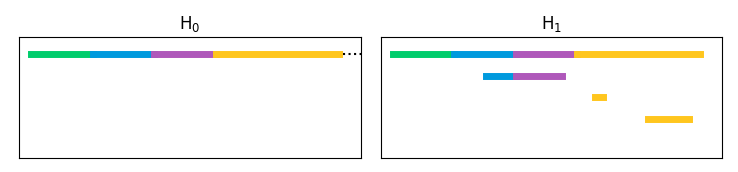
\includegraphics[width=0.8\textwidth]{scripts/figures/scalar_barcode_true.png}
  \caption{A scalar field on a 2D domain and its persistence barcode.}
\end{figure}


\section{Summary}\label{sec:summary}
% !TeX root = ../main.tex

% Homology provides a collection of invariants that represent global properties of a space.
% Under specific assumptions the presence of a property can be assumed when the space itself is largely unknown.
% Then, given a sample of an unknown space satisfying these assumptions, once can use the homology of the sample in order to confirm it is representative of the space with respect to that property.
%
% The Topological Coverage Criterion (TCC) is one example of this technique in which homology can be used in order to verify that a collection of subsets provided by a sample covers the space.
% Specifically, by assuming the top dimensional relative homology is known one can check that of the sample is what we expect in order to certify coverage by relating the top dimensional relative to the boundary of a space to the zero dimensional homology of the complement.

% The assumptions made about the boundary are central to the TCC.
% While it certainly demonstrates an interesting application of homology to coordinate-free sensor networks these assumptions are unrealistic in practice.
% Specifically, it requires that sensors are capable of detecting the physical presence of a boundary.
% In a coordinate-free setting, where sensors are unable to measure distance nor communicate their coordinates, this requirement seems unnatural.

We will re-cast the TCC as a way to verify that a collection of sample points can adequately approximate an unknown function in an unknown space.
Consider the application to sensor networks as an example, where we take our sample points as sensors dropped in an unknown environment.
We now endow our sensors with the ability to measure some unknown quantity that is related to metric of the space in a specific way (Lipschitz).
In this way we can replace the requirement that sensors can detect the presence of the true topological boundary with assumptions about the function itself.
Indeed, these assumptions could relate the behavior of the function to the topological boundary of the space.
However, the condition holds for any subset which ``surrounds'' the space in a specific sense~\cite{cavanna2017when}.

The TCC uses these assumptions to make the \emph{relative} homology known.
Specifically, we can confirm coverage of the ``interior'' of the space by effectively quarantining the surrounding space we take homology with respect to.
We take this property of relative homology, which can be understood in terms of excision, to its logical extreme.
We consider the case in which we have incomplete data for a particular sub-levelset of the function.
Returning to our sensor network analogy, suppose our sensors measure heat, or some other volatile quantity, and cannot approach a region without failing.
By properly isolating the region, taken as a sub-levelset of the function, we can confirm that the sample we have is topologically representative of the region near, and above this sub-levelset.
We can then re-use the same machinery that was used to verify coverage to analyze a \emph{part} of the function in a very specific way.

% In a superficial sense, the assumptions and machinery required to approximate a function's persistent homology are precisely those confirmed and constructed in the TCC. %\footnote{\textbf{TODON} worst sentence ever, but exactly what I want to say. Also I stole ``superficial'' from your intro because it's perfect. Maybe some of your intro can fill this in.}.

While the approximation of a function's persistent homology is well studied in general~\cite{chazal08towards}, the presence of incomplete data can severely impact the quality of the approximation.
This is primarily due to the nature of homology as a measure of \emph{global} structure.
While the obvious solution is to simply remove the un-verified data, the question of what precisely this would approximate is important to consider.
By simply restricting the function to the verified \emph{super}-levelset we accept that there may be global structure to the function itself that we are missing.
If we are then provided with the missing data it may prove more difficult to reconstruct the full diagram in this case.

We consider the persistent homology relative to a sub-levelset as a \emph{truncation} of the full diagram.
That is, beyond a certain point the full diagram remains unchanged, allowing for possible reconstruction.
This is in comparison to the persistent homology of the \emph{restricted} function, which fills in missing global structure with potentially spurious features.
Indeed, it can be shown that the truncated diagram is captured by the restriction in a specific way~\cite{cohen09extending, desilva11duality}.
We hypothesize that the approximation of the restricted function directly provides a worse interleaving with the corresponding subset of the \emph{full} diagram

We will first provide some background on important topological, geometric, and algebraic structures required for our re-formulation of the TCC, and the approximation of the truncated diagram.
We then introduce the notion of a \emph{surrounding set}, or pair, which will be central in or re-formulation of the TCC.
Section~\ref{sec:middle} establishes the algebraic tools that will be used to approximate the truncated diagram, and discuss how they fit in the context of the TCC.
After providing the proof of the interleaving in Section~\ref{sec:interleaving} we discuss the meaning and significance of truncated diagrams, and compare them to the diagrams of restricted functions.


\begin{figure}[htbp]
  \centering
  % 
\includegraphics[trim=50 190 0 200, clip, scale=0.2]{scripts/figures/scalar.png}
  % 
\includegraphics[trim=100 25 75 0, clip, angle=280, scale=0.25]{scripts/figures/scalar_contour.png}
  
\includegraphics[trim=200 200 200 200, clip, width=0.5\textwidth]{scripts/figures/surf/side.png}
  
\includegraphics[trim=200 0 200 200, clip, width=0.3\textwidth]{scripts/figures/surf/top.png}
  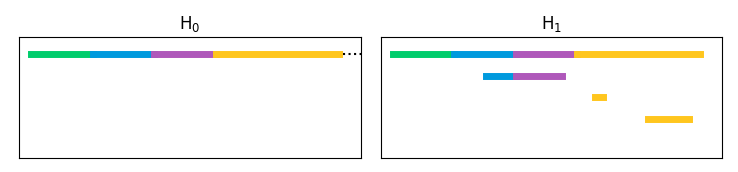
\includegraphics[scale=0.75]{scripts/figures/scalar_barcode_true.png}
  % \includegraphics[trim=0 310 270 0, clip, scale=0.8]{scripts/figures/scalar_restricted.png}
  % \includegraphics[scale=0.55]{scripts/figures/scalar_barcode_super_0.png}
  % \includegraphics[scale=0.55]{scripts/figures/scalar_barcode_sub_1.png}
\end{figure}


\section{The Topological Coverage Criterion (TCC)}\label{sec:tcc}
% !TeX root = ../../main_socg.tex

% The TCC uses the top-dimensional relative homology of a space $D$ with respect to its boundary $B$ to provide a computable condition for coverage.
% Under certain conditions Alexander Duality can be used to relate this to the number of connected components of its complement in some larger space $\X$.
% % Under certain conditions it can be shown that the rank of this group is equal to the number of connected components of its complement in some larger space $\X$ by Alexander Duality.
% One can then check if a collection of subsets covers the space by comparing the number of connected components of its complement to that of the space---holes in the cover will appear as additional components in the complement space.
% As we cannot compute the number components of the complement space from a sample directly, the TCC uses duality to recover it from the top dimensional relative homology.

A positive result from the TCC requires that we have a subset of our cover to serve as the boundary.
That is, the the condition not only checks that we have coverage, but also that we have a pair of spaces that reflects the pair $(D, B)$ topologically.
We call such a pair a \emph{surrounding pair} defined in terms of separating sets.
It has been shown that the TCC can be stated in terms of these surrounding pairs~\cite{cavanna2017when}.
Moreover, this work made assumptions directly in terms of the \emph{zero dimensional} persistent homology of the domain close to the boundary.
This allows allows us enough flexibility to define our surrounding set as a sublevel of a $c$-Lipschitz function $f$ and state our assumptions in terms of its persistent homology.

\begin{definition}[Surrounding Pair]
  Let $X$ be a topological space and $(D,B)$ a pair in $X$.
  The set $B$ \textbf{surrounds $D$ in $X$} if $B$ separates $X$ with the pair $(D\setminus B, X\setminus D)$.
  We will refer to such a pair as a \textbf{surrounding pair in $X$}.
\end{definition}

The following lemma generalizes the proof of the TCC as a property of surrounding sets.%TODO, its proof can be found in the \fullversion.

\begin{lemma}\label{lem:coverage}
  Let $(D, B)$ be a surrounding pair in $X$ and $U\subseteq D$, $V\subseteq U\cap B$ be subsets.
  Let $\ell: \hom_0(X\setminus B, X\setminus D)\to \hom_0(X\setminus V, X\setminus U)$ be induced by inclusion.

  If $\ell$ is injective then $D\setminus B\subseteq U$ and $V$ surrounds $U$ in $D$.
\end{lemma}

We now combine these results on the homology of surrounding pairs with information about both $\X$ as a metric space and our function.
Let $(\X,\dist)$ be a metric space and $D\subseteq \X$ be a compact subspace.
For a $c$-Lipschitz function $f : D\to \R$ we introduce a constant $\omega$ as a threshold that defines our ``boundary'' as a sublevel set $B_\omega$ of the function $f$.
Let $P$ be a finite subset of $D$ and $\zeta\geq\delta > 0 $ and be constants such that $P^\delta\subseteq \intr_\X(D)$.
Here, $\delta$ will serve as our communication radius where $\zeta$ is reserved for use in Section~\ref{sec:middle}.
  \footnote{We will set $\zeta = 2\delta$ in the proof of our interleaving with Rips complexes but the TCC holds for all $\zeta\geq\delta$.}

\begin{lemma}\label{lem:psurj}
  Let $i : \hom_0(\cmp{\QQ^\of}, \cmp{P^\of})\to \hom_0(\cmp{\Q^\of}, \cmp{P^\delta})$.

  If $\B$ surrounds $D$ in $\X$ then $\dim~\hom_0(\cmp{\B}, \cmp{D})\geq \rk~i$.
\end{lemma}
\begin{proof}
  Choose a basis for $\im~i$ such that each basis element is represented by a point in $P^\of\setminus \QQ^\of$.
  Let $x\in P^\of\setminus \QQ^\of$ be such that $i[x] \neq 0$.
  So there exits some $p\in P$ such that $\dist(p, x) < \delta$ and $p\notin \QQ$, otherwise $x\in\QQ^\of$.
  Therefore, because $f$ is $c$-Lipschitz,
  \[ f(x)\geq f(p) - c\dist(x, p) > \fenn - c\of =\omega.\]

  So $x\in\cmp{\B}$ and, because $x\in P^\of\subseteq D$, $x\in D\setminus \B$.
  Because $i$ and $\ell : \hom_0(\cmp{\B}, \cmp{D})\to \hom_0(\cmp{\Q^\of}, \cmp{P^\of})$ are induced by inclusion $\ell[x] = i[x]\neq 0$ in $\hom_0(\cmp{\Q^\of}, \cmp{P^\of})$.
  That is, every element of $\im~i$ has a preimage in $\hom_0(\cmp{\B}, \cmp{D})$, so we may conclude that $\dim~\hom_0(\cmp{\B}, \cmp{D})\geq \rk~i$.
\end{proof}

Note that, while there is a surjective map from $\hom_0(\cmp{\B}, \cmp{D})$ to $\im~i$ this map is not necessarily induced by inclusion.
We therefore must introduce a larger space $B_{\omega+c(\delta+\zeta)}$ that contains $\QQ^\of$ in order to provide a criteria for the injectivity of $\ell : \hom_0(\cmp{\B}, \cmp{D})\to\hom_0(\cmp{\Q^\of}, \cmp{P^\of})$ in terms of $\rk~i$.
We have the following commutative diagrams of inclusion maps the induced maps between complements in $\X$.

% \[ \begin{tikzcd}
%   (P^\of, \Q^\of) \arrow[hookrightarrow]{r}\arrow[hookrightarrow]{d} &
%   (P^\of, \QQ^\of) \arrow[hookrightarrow]{d} \\
%   %
%   (D, \bb) \arrow[hookrightarrow]{r} &
%   (D, B_{\omega+c(\delta+\zeta)}),
% \end{tikzcd}\begin{tikzcd}
%   (\cmp{B_{\omega+c(\delta+\zeta)}},\cmp{D})\arrow[hookrightarrow]{d}\arrow[hookrightarrow]{r} &
%   (\cmp{\bb}, \cmp{D}) \arrow[hookrightarrow]{d}\\
%   %
%   (\cmp{\QQ^\of}, \cmp{P^\of}) \arrow[hookrightarrow]{r} &
%   (\cmp{\Q^\of}, \cmp{P^\of}).
% \end{tikzcd}\]

% \begin{equation}\label{dgm:1}\begin{tikzcd}
%   \hom_0(\cmp{B_{\omega+c(\delta+\zeta)}},\cmp{D})\arrow{d}{m} \arrow{r}{j} &
%   \hom_0(\cmp{\bb}, \cmp{D}) \arrow{d}{\ell} \\
%   %
%   \hom_0(\cmp{\QQ^\of}, \cmp{P^\of}) \arrow{r}{i} &
%   \hom_0(\cmp{\Q^\of}, \cmp{P^\of}).
% \end{tikzcd}\end{equation}

\begin{equation}\label{dgm:1}
\begin{tikzcd}
  (P^\of, \Q^\of) \arrow[hookrightarrow]{r}\arrow[hookrightarrow]{d} &
  (P^\of, \QQ^\of) \arrow[hookrightarrow]{d} \\
  %
  (D, \bb) \arrow[hookrightarrow]{r} &
  (D, B_{\omega+c(\delta+\zeta)}),
\end{tikzcd}
\begin{tikzcd}
  \hom_0(\cmp{B_{\omega+c(\delta+\zeta)}},\cmp{D})\arrow{d}{m} \arrow{r}{j} &
  \hom_0(\cmp{\bb}, \cmp{D}) \arrow{d}{\ell} \\
  %
  \hom_0(\cmp{\QQ^\of}, \cmp{P^\of}) \arrow{r}{i} &
  \hom_0(\cmp{\Q^\of}, \cmp{P^\of}).
\end{tikzcd}\end{equation}

\paragraph*{Assumptions}

We will first require the map $\hom_0(D\setminus B_{\omega+c(\delta+\zeta)}\hookrightarrow D\setminus B_\omega)$ to be \emph{surjective}---as we approach $\omega$ from \emph{above} no components \emph{appear}.
This ensures that the rank of the map $j$ is equal to the dimension of $\dim~\hom_0(\cmp{B_\omega}, \cmp{D})$ so our map $\ell$ induced by inclusion depends only on $\hom_0(\cmp{B_\omega}, \cmp{D})$ and $\im~i$.
% That is, in terms of $\omega$ as a super-levelset monotonically decreasing, no components \emph{apear} right \emph{before} $\omega$.
% We note that, for a function in two dimensions, this translates to $1$-dimensional features disappearing right after $\omega$ in the sub-levelset filtration, as shown in Figure~\ref{fig:assumption1}.

We also assume that $\hom_0(D\setminus B_\omega\hookrightarrow D\setminus B_{\omega-c(\delta+\zeta)})$ is \emph{injective}---as we move away from $\omega$ moving \emph{down} no components \emph{disappear}.
Lemma~\ref{lem:assumption2} uses Assumption 2 to provide a computable upper bound on $\rk~j$.%TODO, its proof can be found in the \fullversion.
% Once again, in terms of $\omega$ as a superlevel set monotonically decreasing, no components \emph{disappear} right \emph{after} $\omega$.
% Once again, for a function in two dimensions, this translates to features in dimension 1 appearing before $\omega$ is the sublevel set filtration, as shown in Figure~\ref{fig:assumption2}.

\begin{figure}[htbp]\label{fig:assumption1}
  \centering
  
\includegraphics[trim=200 300 200 200, clip, width=0.3\textwidth]{scripts/figures/surf/ass2_B_side.png}
  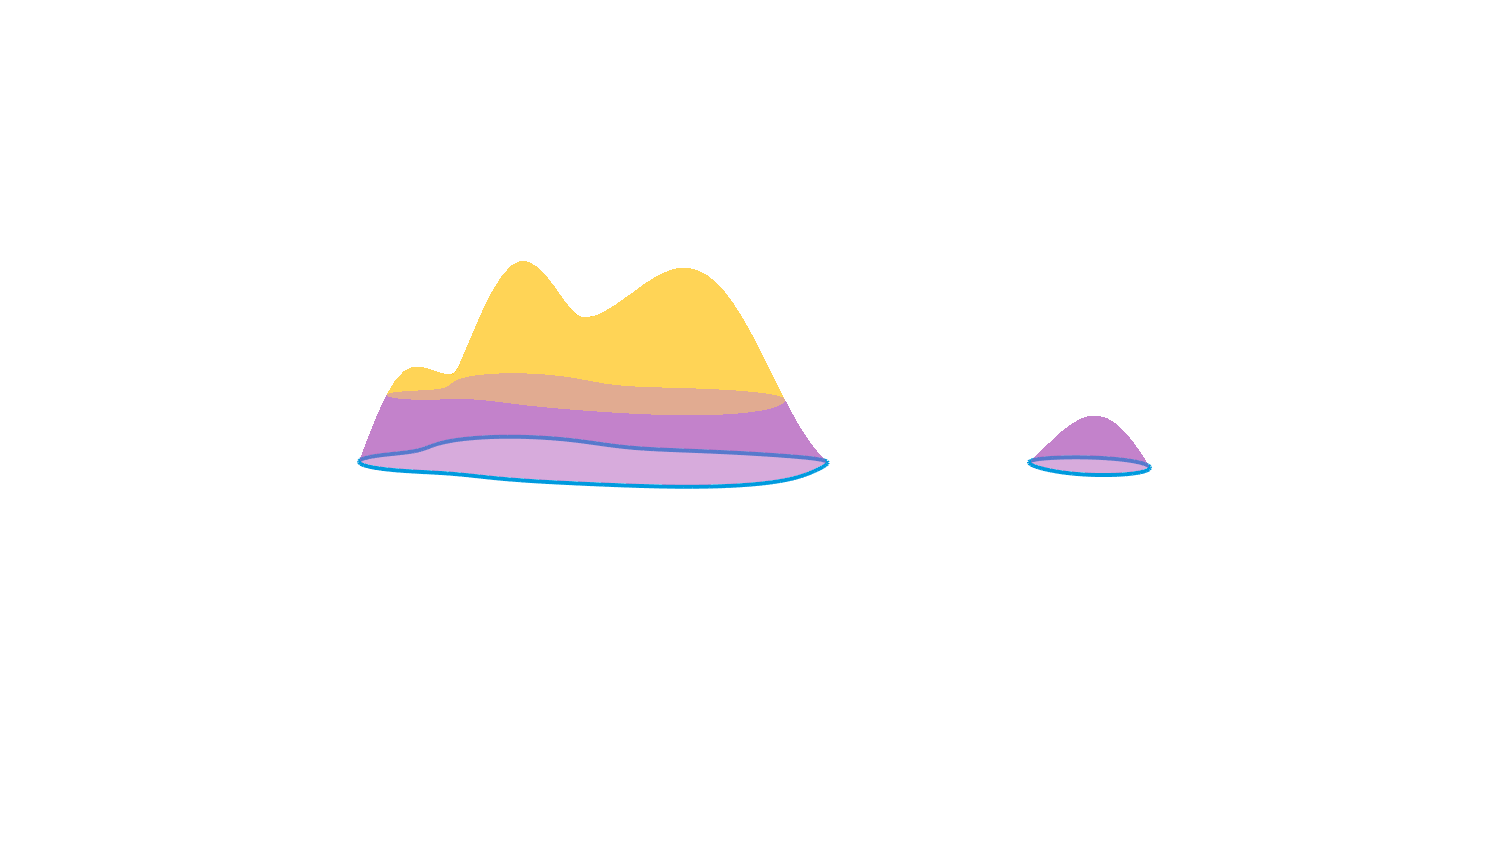
\includegraphics[trim=200 300 200 200, clip, width=0.3\textwidth]{scripts/figures/surf/ass1_C_side.png}
  
\includegraphics[trim=200 300 200 200, clip, width=0.3\textwidth]{scripts/figures/surf/ass1_D_side.png}
  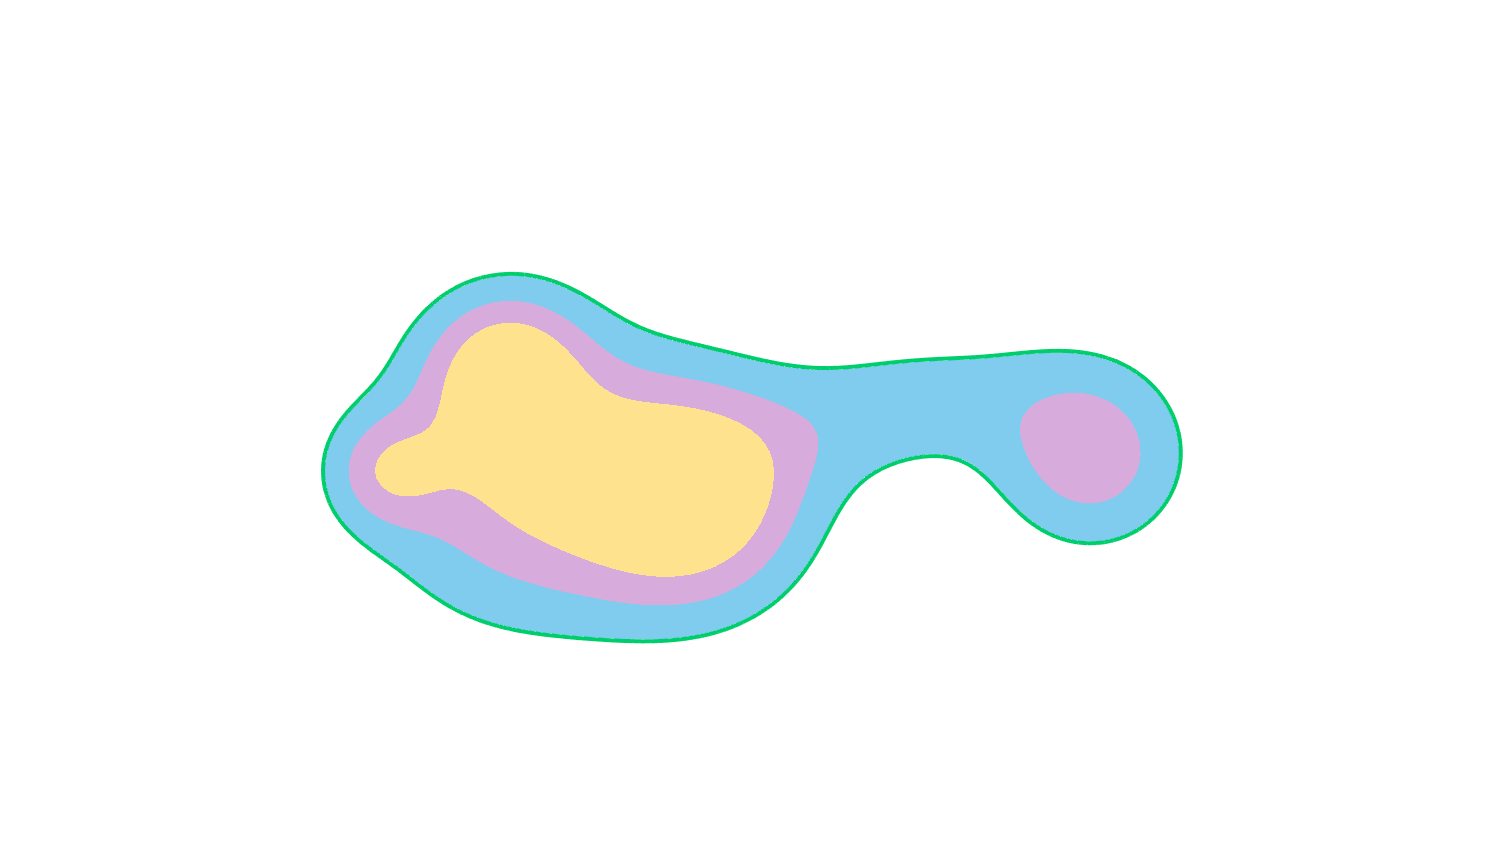
\includegraphics[trim=300 100 200 200, clip, width=0.3\textwidth]{scripts/figures/surf/ass2_B_top.png}
  
\includegraphics[trim=300 150 300 200, clip, width=0.3\textwidth]{scripts/figures/surf/ass1_C_top.png}
  
\includegraphics[trim=300 150 300 200, clip, width=0.3\textwidth]{scripts/figures/surf/ass1_D_top.png}
  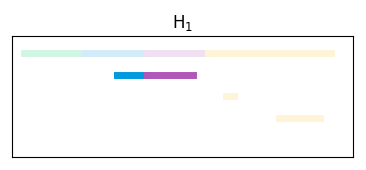
\includegraphics[width=0.5\textwidth]{scripts/figures/scalar_barcode_H1-masked.png}
  \caption{The blue level set does not satisfy either assumption as the smaller component is not in the inclusion from blue to green and it ``pinched out'' in the yellow region. This can be seen in the barcode shown as a feature that is born in the blue region and dies in the purple region.}
\end{figure}

% \begin{figure}[htbp]\label{fig:assumption2}
%   \centering
%   
\includegraphics[trim=200 300 200 200, clip, width=0.5\textwidth]{scripts/figures/surf/ass2_C_side.png}
%   
\includegraphics[trim=300 200 200 200, clip, width=0.3\textwidth]{scripts/figures/surf/ass2_C_top.png}
%   
\includegraphics[trim=200 300 200 200, clip, width=0.5\textwidth]{scripts/figures/surf/ass2_B_side.png}
%   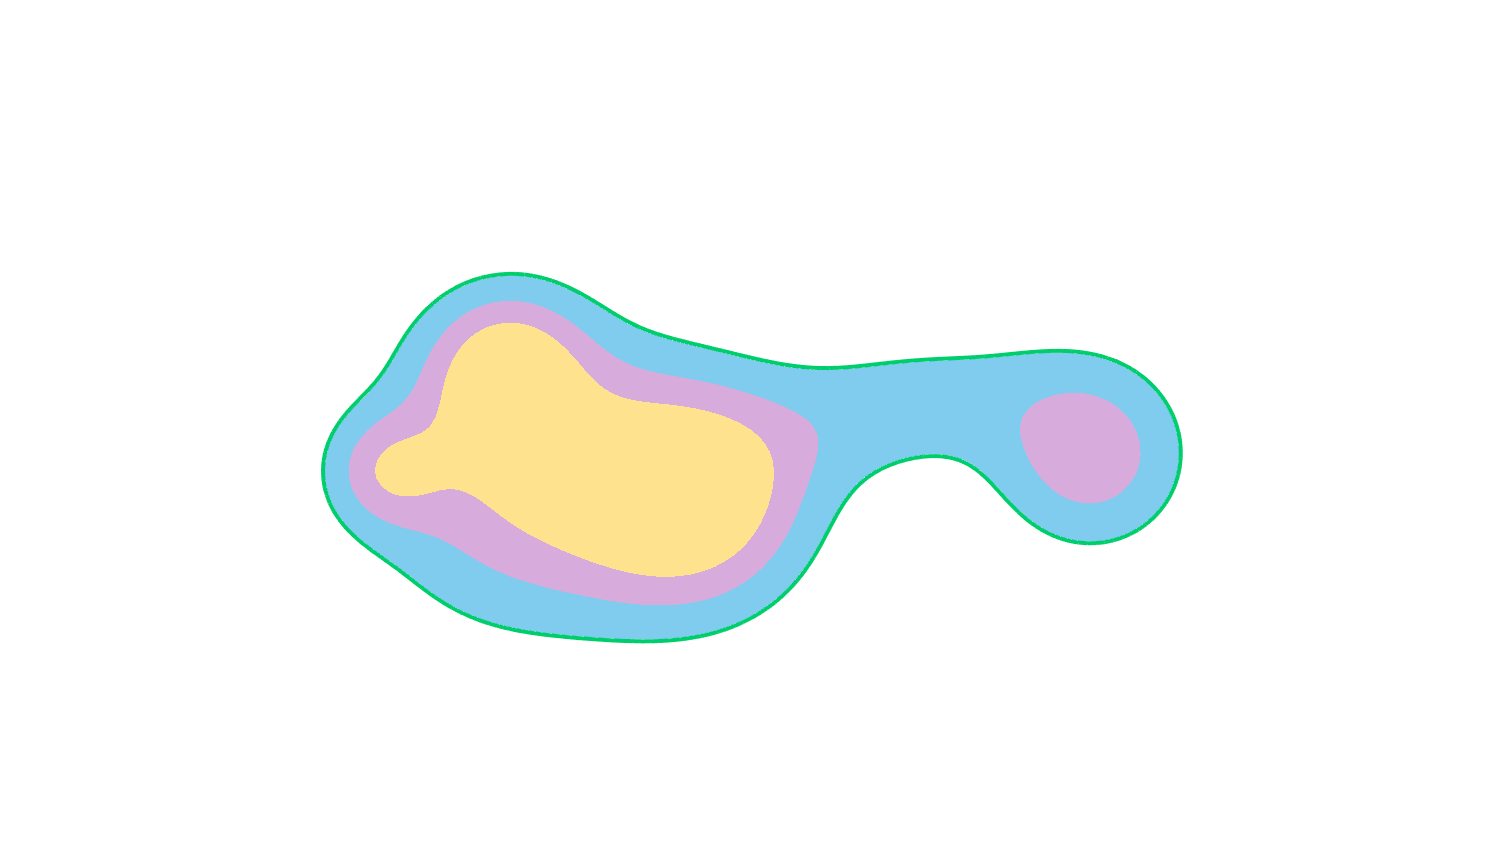
\includegraphics[trim=300 200 200 200, clip, width=0.3\textwidth]{scripts/figures/surf/ass2_B_top.png}
%   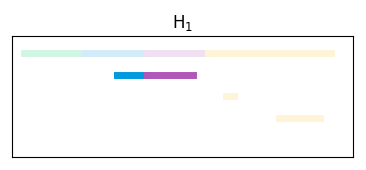
\includegraphics[scale=0.7]{scripts/figures/scalar_barcode_H1-masked.png}
%   \caption{\textbf{(Assumption 2)} The blue levelset does not satisfy Assumption 2 as the smaller component is not in the inclusion from blue to green.}
%           % This can be seen in the second feature of the barcode shown as a feature which is born in the blue region.}
% \end{figure}

\begin{lemma}\label{lem:assumption2}
  If $\hom_0(D\setminus B_\omega\hookrightarrow D\setminus B_{\omega+c(\delta+\zeta)})$ is injective and each component of $D\setminus B_\omega$ contains a point in $P$ then $\dim~\hom_0(\rips^\delta(P\setminus Q_{\omega-c\zeta})) \geq \dim~\hom_0(D\setminus B_\omega)$.
\end{lemma}

\paragraph*{Nerves and Duality}

Recall that the Nerve Theorem states that for a good open cover$\cU$ of a space $X$ the inclusion map from the \emph{Nerve} of the cover to the space $\N(\cU)\hookrightarrow X$ is a homotopy equivalence.\footnote{In a good open cover every nonempty intersection of sets in the cover is contractible.}
The Persistent Nerve Lemma~\cite{chazal08towards} states that this homotopy equivalence commutes with inclusion on the level of homology.
We note that the standard proof of the Nerve Theorem~\cite{kozlov07combinatorial}, and therefore the Persistent Nerve Lemma~\cite{chazal08towards}, extends directly to pairs of good open covers $(\cU, \cV)$ of pairs $(X, Y)$ such that $\cV$ is a subcover of $\cU$.\footnote{$\{V_i\}_{i\in I}$ is a subcover of $\{U_i\}_{i\in I}$ if $V_i\subseteq U_i$ for all $i\in I$.}

Recalling the definition of the strong convexity radius $\varrho_D$ (see Chazal et al.~\cite{chazal09analysis}) $\cU$ is a good open cover whenever $\varrho_D > \e$.
As the \v Cech complex is the Nerve of a cover by a union of balls we will let $\N_w^\e : \hom_k(\cech^\e(P,Q_w))\to \hom_k(P^\e, Q_w^\e)$ denote the isomorphism on homology provided by the Nerve Theorem for all $k$, $w\in\R$ and $\e < \varrho_D$.

Under certain conditions Alexander Duality provides an isomorphism between the $k$ relative cohomology of a compact pair in an orientable $d$-manifold $\X$ with the $d - k$ dimensional homology of their complements in $\X$ (see Spanier~\cite{spanier1989algebraic}).
For finitely generated (co)homology over a field the Universal Coefficient Theorem can be used with Alexander Duality to give a natural isomorphism $\xi_w^\e : \hom_d(P^\e,Q_w^\e)\to \hom_0(D\setminus Q_w^\e, D\setminus P^\e)$.\footnote{For the construction of this isomorphism see the \fullversion.}
This isomorphism holds in the specific case when $P^\e\subseteq \intr_\X(D)$ and $D\setminus P^\e$, $D\setminus Q_w^\e$ are locally contractible.
We therefore provide the following definition for ease of exposition.
\begin{definition}[$(\delta,\zeta,\omega)$-Sublevel Sample]
  For $\zeta\geq \delta > 0$, $\omega\in\R$, and a $c$-Lipschitz function $f: D\to \R$ a finite point set $P\subset D$ is said to be a \textbf{$(\delta, \zeta, \omega)$-sublevel sample} of $f$ if every component of $D\setminus B_\omega$ contains a point in $P$, $P^\delta\subset\intr_\X(D)$, and $D\setminus P^\delta$, $D\setminus Q_{\omega-c\zeta}^\delta$, and $D\setminus Q_{\omega+c\delta}^\delta$ are locally path connected in $\X$.
\end{definition}
Because this isomorphism is natural and the isomorphism provided by the Nerve Theorem commutes with maps induced by inclusion the composition $\xi\N_w^\e := \xi_w^\e\circ\N_w^\e$ gives an isomorphism that commutes with maps induced by inclusion for all $w\in\R$ and $\e < \varrho_D$.

\begin{theorem}[Algorithmic TCC]\label{thm:algo_tcc}
  Let $\X$ be an orientable $d$-manifold and let $D$ be a compact subset of $\X$.
  Let $f : D\to\R$ be $c$-Lipschitz function and $\omega\in\R$ and $\delta\leq\zeta < \varrho_D$ be constants such that $P\subset D$ is a $(\delta,\zeta,\omega)$-sublevel sample of $f$ and $B_{\omega - c(\zeta +\delta)}$ surrounds $D$ in $\X$.

  If $\hom_0(D\setminus B_{\omega+c(\delta+\zeta)}\hookrightarrow D\setminus B_\omega)$ is surjective, $\hom_0(D\setminus B_\omega\hookrightarrow D\setminus B_{\omega+c(\delta+\zeta)})$ is injective, and $\rk~\hom_d(\rips^\delta(P, Q_{\omega -c\zeta})\hookrightarrow \rips^{2\delta}(P, Q_{\omega+c\delta})) \geq \dim~\hom_0(\rips^\delta(P\setminus Q_{\omega-c\zeta}))$ then $D\setminus B_\omega\subseteq P^\delta$ and $Q_{\omega-c\zeta}^\delta$ surrounds $P^\delta$ in $D$.
\end{theorem}
\begin{proof}
  % We have the following commutative diagram
  % \[\begin{tikzcd}
  %   \hom_d(\cech^\delta(P, Q_{\omega-c\zeta})) \arrow{r}{q_{\cech}}\arrow{d}{\N_{\omega-c\zeta}^{\delta}} &
  %   \hom_d(\cech^\delta(P, Q_{\omega+c\delta})) \arrow{d}{\N_{\omega-c\zeta}^\delta}\\
  %   %
  %   \hom_d(P^\delta, Q_{\omega-c\zeta}^\delta))\arrow{r}{q} &
  %   \hom_d(P^\delta, Q_{\omega+c\delta}^\delta).
  % \end{tikzcd}\]
  % where vertical maps are isomorphisms provided by the Nerve Theorem and horizontal maps are induced by inclusions.

  Because $P$ is a $(\delta, \zeta, \omega)$-sublevel sample we have isomorphisms $\xi\N_{\omega-c\zeta}^\delta$ and $\xi\N_{\omega+c\delta}^\delta$ that commute with $q_{\cech} : \hom_d(\cech^{\delta}(P, Q_{\omega-c\zeta}))\to\hom_d(\cech^{2\delta}(P, Q_{\omega+c\delta}))$ and $i : \hom_0(D\setminus Q_{\omega+c\delta}^\delta, D\setminus P^\delta)\to \hom_0(D\setminus Q_{\omega-c\zeta}^\delta, D\setminus P^\delta)$.
  Let $q_{\rips} : \hom_d(\rips^{\delta}(P, Q_{\omega-c\zeta}))\to\hom_d(\rips^{2\delta}(P, Q_{\omega+c\delta}))$ be induced by inclusion.
  Then $\rk~q_{\cech} \geq\rk~q_{\rips}$ as $q_{\rips}$ factors through $q_{\cech}$.
  As we have assumed $\hom_0(D\setminus B_\omega\hookrightarrow D\setminus B_{\omega-c(\delta+\zeta)})$ Lemma~\ref{lem:assumption2} implies $\dim~\hom_0(\rips^\delta(P\setminus Q_{\omega-c\zeta}))\geq \dim~\hom_0(D\setminus B_\omega)$.
  It follows that, whenever $\rk~q_{\rips} \geq \dim~\hom_0(\rips^\delta(P\setminus Q_{\omega-c\zeta}))$, we have
  \[ \rk~i = \rk~q_{\cech} \geq \rk~q_{\rips} \geq \dim~\hom_0(\rips^\delta(P\setminus Q_{\omega-c\zeta})) \geq \dim~\hom_0(D\setminus B_\omega).\]

  Because $j$ is surjective by hypothesis $\rk~j = \dim~\hom_0(\cmp{\B},\cmp{D}) = \dim~\hom_0(D\setminus B_\omega)$ so $\rk~j\geq \rk~i$ by Lemma~\ref{lem:psurj}.
  As we have shown $\rk~i\geq \dim~\hom_0(D\setminus B_\omega)$ it follows that $\rk~j = \rk~i$.
  Because $P$ is a finite point set we know that $\im~i$ is finite-dimensional and, because $\rk~i = \rk~j$, $\im~j=\hom_0(\cmp{\B}, \cmp{D})$ is finite dimensional as well.
  So $\im~j$ is isomorphic to $\im~i$ as a subspace of $\hom_0(\cmp{\Q^\of}, \cmp{P^\of})$ which, because $j$ is surjective, requires the map $\ell$ to be injective.
  Therefore $D\setminus\bb\subseteq P^\of$ and $\Q^\of$ surrounds $P^\of$ in $D$ by Lemma~\ref{lem:coverage}.
  %, Lemma~\ref{lem:cov_surrounds}.
  % As $j : \hom_0(D\setminus B_{\omega+c(\delta+\zeta)})\to \hom_0(D\setminus B_\omega)$ is surjective by assumption $\rk~j = \dim~\hom_0(D\setminus B_\omega)$, so $D\setminus B_\omega\subseteq P^\delta$ and $Q_{\omega-c\zeta}^\delta$ surrounds $P^\delta$ in $D$ by Theorem~\ref{thm:geo_tcc} as desired.
\end{proof}

% % !TeX root = ../../main.tex

% Let $D$ be a compact subset of $\X$.
% Let $\dist(x, y) = \|x - y\|$ denote the distance between points $x,y\in D$ as a subspace of $\X$.
% For $A\subset D$ and $x\in D$ let
% \[\dist_A(x) = \min_{a\in A}\dist(x, a)\]
% denote the distance from $x$ to the set $A$.
% We will use open metric balls restricted to $D$ with the subspace topology
% \[\ball_\e(x) = \{y\in D\mid \dist(x, y) < \e\}\]
% and offsets
% \[A^\e = \{x\in D\mid \dist_A(x) < \e\}.\]

We now combine these results on the homology of surrounding pairs with information about both $\X$ as a metric space as well as a function of interest.
In the following section we will apply these results to a computable variation which requires only pair-wise connectivity information via the Vietoris-Rips complex.

Let $(\X,\dist)$ be a metric space and $D\subseteq \X$ be a compact subspace.
Let $f : D\to \R$ be a $c$-Lipschitz function on $D$ and $B_\alpha = f^{-1}((-\infty, a])$ denote the $\alpha$-sublevel set of $f$ for $\alpha\in\R$.
We introduce a constant $\omega$ as a threshold that defines our ``boundary'' as a sub-levelset of the function $f$.
The following sections will explore both the challenges of computing as well as the meaning of the persistent homology of a function modulo a sub-levelset.

Let $P$ be a finite subset of $D$ and $Q_\alpha := P\cap B_\alpha$ for $\alpha\in\R$.
Let $\zeta\geq\delta > 0 $ and $\omega\in \R$ be constants such that $P^\delta\subseteq D$.
Here, $\delta$ will serve as our communication radius where $\zeta$ is reserved as a constant for use in Section~\ref{sec:interleaving}.
Unlike previous variations of the TCC we do not require a change of scale in the geometric case.
Instead, we will enforce regularity close to the sub-levelset $B_\omega$ in terms of sub-levelsets $B_{\omega-c(\delta+\zeta)}$ and $B_{\omega+c(\delta+\zeta)}$.
Not only is this a more natural assumption, but it also allows us to replace the requirement that sensors detect the physical presence of a boundary with a threshold on the function values they observe.

\begin{lemma}\label{lem:psurj}
  Let $i : \hom_0(\cmp{\QQ^\of}, \cmp{P^\of})\to \hom_0(\cmp{\Q^\of}, \cmp{P^\delta})$.

  If $\B$ surrounds $D$ in $\X$ then $\dim~\hom_0(\cmp{\B}, \cmp{D})\geq \rk~i$.
\end{lemma}
\begin{proof}
  Choose a basis for $\im~i$ such that each basis element is represented by a point in $P^\of\setminus \QQ^\of$.
  Let $x\in P^\of\setminus \QQ^\of$ be such that $i[x] \neq 0$.
  So there exits some $p\in P$ such that $\dist(p, x) < \delta$ and $p\notin \QQ$, otherwise $x\in\QQ^\of$.
  Therefore, because $f$ is $c$-Lipschitz,
  \[ f(x)\geq f(p) - c\dist(x, p) > \fenn - c\of =\omega.\]

  So $x\in\cmp{\B}$ and, because $x\in P^\of\subseteq D$, $x\in D\setminus \B$.
  Because $i$ and $\ell : \hom_0(\cmp{\B}, \cmp{D})\to \hom_0(\cmp{\Q^\of}, \cmp{P^\of})$ are induced by inclusion $\ell[x] = i[x]\neq 0$ in $\hom_0(\cmp{\Q^\of}, \cmp{P^\of})$.
  That is, every element of $\im~i$ has a preimage in $\hom_0(\cmp{\B}, \cmp{D})$, so we may conclude that $\dim~\hom_0(\cmp{\B}, \cmp{D})\geq \rk~i$.
\end{proof}

Note that, while there is a surjective map from $\hom_0(\cmp{\B}, \cmp{D})$ to $\im~i$ this map is not necessarily induced by inclusion, as $\QQ^\of\not\subseteq \B$.
We therefore must introduce a larger space $B_{\omega+c(\delta+\zeta)}$ that contains $\QQ^\of$ in order to provide a computable criteria for the injectivity of $\ell : \hom_0(\cmp{\B}, \cmp{D})\to\hom_0(\cmp{\Q^\of}, \cmp{P^\of})$.

\[ \begin{tikzcd}
  (P^\of, \Q^\of) \arrow[hookrightarrow]{r}\arrow[hookrightarrow]{d} &
  (P^\of, \QQ^\of) \arrow[hookrightarrow]{d} \\
  %
  (D, \bb) \arrow[hookrightarrow]{r} &
  (D, B_{\omega+c(\delta+\zeta)}),
\end{tikzcd}\begin{tikzcd}
  (\cmp{B_{\omega+c(\delta+\zeta)}},\cmp{D})\arrow[hookrightarrow]{d}\arrow[hookrightarrow]{r} &
  (\cmp{\bb}, \cmp{D}) \arrow[hookrightarrow]{d}\\
  %
  (\cmp{\QQ^\of}, \cmp{P^\of}) \arrow[hookrightarrow]{r} &
  (\cmp{\Q^\of}, \cmp{P^\of}).
\end{tikzcd}\]

\begin{equation}\label{dgm:1}\begin{tikzcd}
  \hom_0(\cmp{B_{\omega+c(\delta+\zeta)}},\cmp{D})\arrow{d}{m} \arrow{r}{j} &
  \hom_0(\cmp{\bb}, \cmp{D}) \arrow{d}{\ell} \\
  %
  \hom_0(\cmp{\QQ^\of}, \cmp{P^\of}) \arrow{r}{i} &
  \hom_0(\cmp{\Q^\of}, \cmp{P^\of}).
\end{tikzcd}\end{equation}

\begin{theorem}[Geometric TCC]\label{thm:geo_tcc}
  Let $D$ be a compact subset of $\X$ and $f : D\to\R$ be $c$-Lipschitz function.
  Let $\omega\in\R$, $\of > 0$ be constants such that $\B$ surrounds $D$ in $\X$.
  Let $P\subset D$ be a finite collection of points and $Q_\alpha := P\cap B_\alpha$ for $\alpha\in\R$.
  Let $j : \hom_0(\cmp{B_{\omega+c(\delta+\zeta)}},\cmp{D})\to \hom_0(\cmp{\B},\cmp{D})$ and $i : \hom_0(\cmp{\QQ^\of}, \cmp{P^\of})\to \hom_0(\cmp{\Q^\of}, \cmp{P^\of})$ be induced by inclusion.

  If $j$ is surjective and $\rk~i\geq \rk~j$ then $D\setminus \B\subseteq P^\of$ and $\Q^\of$ surrounds $P^\of$ in $D$.
\end{theorem}
\begin{proof}
  Because $j$ is surjective by hypothesis $\rk~j = \dim~\hom_0(\cmp{\B},\cmp{D})$ so $\rk~j\geq \rk~i$ by Lemma~\ref{lem:psurj}.
  So $\rk~j = \rk~i$ with our assumption that $\rk~i\geq \rk~j$.
  Because $P$ is a finite point set we know that $\im~i$ is finite-dimensional and, because $\rk~i = \rk~j$, $\im~j=\hom_0(\cmp{\B}, \cmp{D})$ is finite dimensional as well.

  So $\im~j$ is isomorphic to $\im~i$ as a subspace of $\hom_0(\cmp{\Q^\of}, \cmp{P^\of})$ which, because $j$ is surjective, requires the map $\ell$ induced by inclusion to be injective.
  Therefore, $D\setminus\bb\subseteq P^\of$ by Lemma~\ref{lem:coverage}, and $\Q^\of$ surrounds $P^\of$ in $D$ by Lemma~\ref{lem:cov_surrounds}.
\end{proof}
 % 57
% % !TeX root = ../../main.tex

For a finite point set $P\subset D$ recall that the \Cech complex $\cech^\e(P)$ is defined to be the Nerve of the open cover $\{\ball_D^\e(p)\}_{p\in P}$.
When $\varrho_D > \e$ this cover is good, and the Nerve Theorem states that $\cech^\e(P)$ is homotopy equivalent to $P^\e$.
That is, we have an isomorphism $\N_w^{\e, k} : \hom_k(\cech^\e(P,Q_w))\to \hom_k(P^\e, Q_w^\e)$ on homology groups that is induced by this homotopy equivalence.

\paragraph{Duality}

The statement of Theorem~\ref{thm:geo_tcc} is in terms of the $0$-dimensional homology of complement spaces makes it difficult, if not impossible, to compute directly.
The following lemma applies a version of duality in (co)homology (see Lemma~\ref{cor:alexander_iso} in the appendix) which equates the $0$-dimensional homology of complements with the $d$-dimensional homology of cover.
This is then combined with isomorphisms provided by the Nerve Theorem in order to give us a computable alternative to the hypothesis of Theorem~\ref{thm:geo_tcc}.

\begin{lemma}\label{lem:duality_apply}
  Let $\X$ be an orientable $d$-manifold let $D$ be a compact subset of $\X$ with strong convexity radius $\varrho_D > \e$.
  Let $P$ be a finite subset of $D$ such that $P^\e\subset \intr_\X(D)$ and $Q\subseteq P$.

  If $D\setminus Q^\e$ and $D\setminus P^\e$ are locally path connected then there is an isomorphism
  \[ \xi\N : \hom_d(\cech^\e(P,Q))\to \hom_0(D\setminus Q^\e, D\setminus P^\e)\]
  that commutes with maps induced by inclusions.
\end{lemma}
\begin{proof}
  Because $Q^\e$ and $P^\e$ are open in $D$ and $D$ is compact in $\X$ the complement $D\setminus Q^\e$ is closed in $D$, and therefore compact in $\X$.
  Moreover, because $P^\e\subset \intr_\X(D)$, $\hom_d(\X\setminus(D\setminus P^\e), \X\setminus(D\setminus Q^\e)) = \hom_d(P^\e, Q^\e)$.
  As we have assumed these complements are locally path connected by assumption we have a natural isomorphism $\xi : \hom_d(P^\e, Q^\e)\to \hom_0(D\setminus Q^\e, D\setminus P^\e)$
  by Lemma~\ref{cor:alexander_iso}.

  Because $\e > \varrho_D$ the covers by metric balls associated with $P^\e$ and $Q^\e$ are good, so we have isomorphisms $\N : \hom_d(\cech^\e(P, Q))\to \hom_d(P^\e, Q^\e)$ for all $Q\subseteq P$ by the Nerve Theorem.
  So the composition $\xi\N := \xi\circ\N$ is an isomorphism.
  Moreover, because $\xi$ is natural and $\N$ commutes with maps induced by inclusions by the persistent nerve lemma the composition $\xi\N$ does as well.
\end{proof}

The requirement that our complements are locally path connected is necessary in order to satisfy the general statement of the duality theorem.
A rigorous investigation of the minimal assumptions that can be made on $\X$ and $D$ is beyond the scope of this paper.
We note that, in practice, it likely suffices to assume that there exists a triangulation of $P^\e$ that is a subcomplex of some refinement of a triangulation of $\X$ (see~\cite{cavanna2017when},~\cite{julian83alexander}).

\paragraph{Rips Approximation}

We would now like to compute the TCC by factoring an inclusion of Rips complexes through that of the \Cech.
This will give us a lower bound on the rank of the map induced on $d$-dimensional homology which can then be used to confirm coverage via Lemma~\ref{lem:duality_apply}.

We have following sequence of homomorphisms induced by inclusions
\[ \hom_k(\rips^\e(P, Q_w))\xrightarrow{J_w^\e}\hom_k(\cech^\e(P, Q_w))\xrightarrow{I_w^\e}\hom_k(\rips^\e(P, Q_w))\]
so that, for any $w\leq z$, $\e\leq\eta < \varrho_D$ and $q_{\rips} : \hom_k(\rips^\e(P, Q_w))\to \hom_k(\rips^{2\eta}(P, Q_z))$, $q_{\cech} : \hom_k(\cech^\e(P, Q_w))\to \hom_k(\cech^{\eta}(P, Q_z))$ induced by inclusions, $q_{\rips}$ factors through $q_{\cech}$ as $q_{\rips} = I_z^\eta\circ q_{\cech}\circ J_w^\e$.

Lemma~\ref{lem:pers_nerve_filt} (see Appendix~\ref{apx:nerves}) adapts the persistent nerve lemma of Chazal et. al.~\cite{chazal08towards} (see Appendix~\ref{apx:nerves}, Lemma~\ref{lem:pers_nerve}) to the relative case.
That is, to show the isomorphisms $\N_w^\e$ and $\N_z^\eta$ commute with maps $q_{\cech}$ and $q : \hom_k(P^\e, Q_w^\e)\to\hom_k(P^\eta, Q_z^\eta)$  induced by inclusion.%, thus $\rk~q = \rk~q_{\cech} \geq \rk~q_{\rips}$.

\begin{theorem}[Algorithmic TCC]\label{thm:algo_tcc}
  Let $\X$ be an orientable $d$-manifold and let $D$ be a compact subset of $\X$.
  Let $f : D\to\R$ be $c$-Lipschitz function and $\omega\in\R$ and $\delta\leq\zeta < \varrho_D$ be constants such that
  $B_{\omega - c(\zeta +\delta)}$ surrounds $D$ in $\X$,
  $\hom_0(D\setminus B_{\omega+c(\delta+\zeta)}\hookrightarrow D\setminus B_\omega)$ is surjective, and
  $\hom_0(D\setminus B_\omega\hookrightarrow D\setminus B_{\omega+c(\delta+\zeta)})$ is injective.
  Let $P\subset \intr_\X(D)$ and suppose $P^\delta$, $Q_{\omega-c\zeta}^\delta$, and $Q_{\omega+c\delta}^\delta$ satisfy the assumptions of Lemma~\ref{lem:duality_apply}.

  If
  \[\rk~\hom_d(\rips^\delta(P, Q_{\omega -c\zeta})\hookrightarrow \rips^{2\delta}(P, Q_{\omega+c\delta})) \geq \dim~\hom_0(\rips^\delta(P\setminus Q_{\omega-c\zeta}))\]
  then $D\setminus B_\omega\subseteq P^\delta$ and $Q_{\omega-c\zeta}^\delta$ surrounds $P^\delta$ in $D$.
\end{theorem}
\begin{proof}
  Assume there exist $p,q \in P\setminus Q_{\omega-c\zeta}$ such that $p$ and $q$ are connected in $\rips^\delta(P\setminus Q_{\omega-c\zeta})$ but not in $D\setminus B_\omega$.
  So the shortest path from $p, q$ is a subset of $(P\setminus Q_{\omega-c\zeta})^\delta$.
  For any $x\in (P\setminus Q_{\omega-c\zeta})^\delta$ there exists some $p\in P$ such that $f(p) > \omega - c\zeta$ and $\dist(p,x) < \delta$.
  Because $f$ is $c$-Lipschitz
  \[ f(x)\geq f(p) - c\dist(x,p) > \omega - c(\delta+\zeta)\]
  so there is a path from $p$ to $q$ in $D\setminus B_{\omega-c(\delta+\zeta)}$, thus $[p] = [q]$ in $\hom_0(D\setminus B_{\omega-c(\delta+\zeta)})$.

  But we have assumed that $[p]\neq[q]$ in $\hom_0(D\setminus B_\omega)$, contradicting our assumption that $\hom_0(D\setminus B_\omega\hookrightarrow D\setminus B_{\omega-c(\delta+\zeta)})$ is injective, so any $p,q$ connected in $\rips^\delta(P\setminus Q_{\omega-c\zeta})$ are connected in $D\setminus B_\omega$.
  That is, $\dim~\hom_0(\rips^\delta(P\setminus Q_{\omega-c\zeta}))\geq \dim~\hom_0(D\setminus B_\omega)$.

  We have the following commutative diagram
  \[\begin{tikzcd}
    \hom_d(\cech^\delta(P, Q_{\omega-c\zeta})) \arrow{r}{q_{\cech}}\arrow{d}{\N_{\omega-c\zeta}^{\delta}} &
    \hom_d(\cech^\delta(P, Q_{\omega+c\delta})) \arrow{d}{\N_{\omega-c\zeta}^\delta}\\
    %
    \hom_d(P^\delta, Q_{\omega-c\zeta}^\delta))\arrow{r}{q} &
    \hom_d(P^\delta, Q_{\omega+c\delta}^\delta).
  \end{tikzcd}\]
  where vertical maps are isomorphisms provided by the Nerve Theorem and horizontal maps are induced by inclusions.
  Therefore, by Lemma~\ref{lem:duality_apply}, the isomorphisms $\xi\N_{\omega-c\zeta}^\delta$ and $\xi\N_{\omega+c\delta}^\delta$ commute with $q_{\cech}$ and $i : \hom_0(D\setminus Q_{\omega+c\delta}^\delta, D\setminus P^\delta)\to \hom_0(D\setminus Q_{\omega-c\zeta}^\delta, D\setminus P^\delta)$.

  Let $q_{\rips} : \hom_d(\rips^{\delta}(P, Q_{\omega+c\delta}))\to\hom_d(\rips^{2\delta}(P, Q_{\omega+c\delta}))$ be induced by inclusion.
  Then $\rk~q_{\cech} \geq\rk~q_{\rips}$ as $q_{\rips}$ factors through $q_{\cech}$.
  As we have shown $\dim~\hom_0(\rips^\delta(P\setminus Q_{\omega-c\zeta}))\geq \dim~\hom_0(D\setminus B_\omega)$ it follows that, whenever $\rk~q_{\rips} \geq \dim~\hom_0(\rips^\delta(P\setminus Q_{\omega-c\zeta}))$ we have
  \begin{align*}
    \rk~i &= \rk~q_{\cech} \geq \rk~q_{\rips}\\
      &\geq \dim~\hom_0(\rips^\delta(P\setminus Q_{\omega-c\zeta}))\\
      &\geq \dim~\hom_0(D\setminus B_\omega).
  \end{align*}

  As $j : \hom_0(D\setminus B_{\omega+c(\delta+\zeta)})\to \hom_0(D\setminus B_\omega)$ is surjective by assumption $\rk~j = \dim~\hom_0(D\setminus B_\omega)$, so $D\setminus B_\omega\subseteq P^\delta$ and $Q_{\omega-c\zeta}^\delta$ surrounds $P^\delta$ in $D$ by Theorem~\ref{thm:geo_tcc} as desired.
\end{proof}
 % 76

\section{From Coverage Testing to the Analysis of Scalar Fields}\label{sec:middle}
% !TeX root = ../../main_socg.tex

Because the TCC only confirms coverage of a \emph{superlevel} set $D\setminus B_\omega$, we cannot guarantee coverage of the entire domain.
Indeed, we could compute the persistent homology of the \emph{restriction} of $f$ to the superlevel set we cover in the standard way~\cite{chazal09analysis}.
Instead, we will approximate the persistent homology of the sublevel set filtration \emph{relative to} the sublevel set $B_\omega$.
In the next section we will discuss an interpretation of the relative diagram that is motivated by examples in Section~\ref{sec:experiments}.

We will first introduce the notion of an extension which will provide us with maps on relative homology induced by inclusion via excision.
However, even then, a map that factors through our pair $(D, B_\omega)$ is not enough to prove an interleaving of persistence modules by inclusion directly.
To address this we impose conditions on sublevel sets near $B_\omega$ which generalize the assumptions made in the TCC.

\subsection{Extensions and Image Persistence Modules}

Suppose $D$ is a subspace of $X$.
We define the extension of a surrounding pair in $D$ to a surrounding pair in $X$ with isomorphic relative homology.

\begin{definition}[Extension]
  If $V$ surrounds $U$ in a subspace $D$ of $X$ let $\ext{V} := V\sqcup (D\setminus U)$ denote the (disjoint) union of the separating set $V$ with the complement of $U$ in $D$.
  The \textbf{extension of $(U, V)$ in $D$} is the pair $(D, \ext{V}) = (U\sqcup (D\setminus U), V\sqcup (D\setminus U)).$
\end{definition}

Lemma~\ref{lem:surround_and_cover} states that we can use these extensions to interleave a pair $(U, V)$ with a sequence of subsets of $(D, B)$.
Lemma~\ref{lem:excision} states that we can apply excision to the relative homology groups in order to get equivalent maps on homology that are induced by inclusions.

\begin{lemma}\label{lem:surround_and_cover}
  Suppose $V$ surrounds $U$ in $D$ and $B'\subseteq B\subset D$.

  If $D\setminus B\subseteq U$ and $U\cap B'\subseteq V\subseteq B'$ then $B'\subseteq \ext{V}\subseteq B$.
\end{lemma}

\begin{lemma}\label{lem:excision}
  Let $(U, V)$ be an open surrounding pair in a subspace $D$ of $X$.

  Then $\hom_k((U\cap A, V)\hookrightarrow (A, \ext{V}))$ is an isomorphism for all $k$ and $A\subseteq D$ with $\ext{V}\subset A$.
\end{lemma}

The TCC uses a nested pair of spaces in order to filter out noise introduced by the sample.
This same technique is used to approximate the persistent homology of a scalar fields~\cite{chazal09analysis}.
As modules, these nested pairs are the images of homomorphisms between homology groups induced by inclusion, which we refer to as image persistence modules.
For a full background on persistence modules, shifted homomorphisms, and interleavings of persistence modules see Chazal et al.~\cite{chazal13structure}.

\begin{definition}[Image Persistence Module]
  The \textbf{image persistence module} of a homomorphism $\Gamma\in\Hom(\UU,\VV)$ is the family of subspaces $\{\Gamma_\alpha :=\im~\gamma_\alpha\}$ in $\VV$ along with linear maps $\{\gamma_\alpha^\beta := v_\alpha^\beta\rest_{\im~\gamma_\alpha} : \Gamma_\alpha\to\Gamma_\beta\}$ and will be denoted by $\im~\Gamma$.
\end{definition}

For a homomorphism $\Gamma\in\Hom(\UU, \VV)$ let $\Gamma[\delta]\in \Hom^{\delta}(\UU, \VV)$ denote the shifted homomorphism defined to be the family of linear maps $\{\gamma_\alpha[\delta] := v_\alpha^\delta\circ \gamma_\alpha : U_\alpha\to V_{\alpha+\delta}\}$.
While we will primarily work with homomorphisms of persistence modules induced by inclusions, in general, defining homomorphisms between images simply as subspaces of the codomain is not sufficient.
Instead, we require that homomorphisms between image modules commute not only with shifts in scale, but also with the functions themselves.

\begin{definition}[Image Module Homomorphism]
  Given $\Gamma\in\Hom(\UU,\VV)$ and $\Lambda\in\Hom(\S,\T)$ along with $(F,G)\in\Hom^\delta(\UU,\S)\times\Hom^\delta(\VV,\T)$ let $\Phi(F, G) : \im~\Gamma\to\im~\Lambda$ denote the family of linear maps $\{\phi_\alpha := g_\alpha\rest_{\Gamma_\alpha} : \Gamma_\alpha\to\Lambda_{\alpha+\delta}\}$.
  $\Phi(F, G)$ is an \textbf{image module homomorphism of degree $\delta$} if the following diagram commutes for all $\alpha\leq\beta$.\footnote{We use the notation $\gamma_\alpha[\beta-\alpha] = v_\alpha^\beta\circ\gamma_\alpha$, $\lambda_\alpha[\beta-\alpha] = t_\alpha^\beta\circ\lambda_\alpha$ to denote the composition of homomorphisms between persistence modules and shifts in scale.}
  \begin{equation}\label{dgm:image_homomorphism}
    \begin{tikzcd}[column sep=large]
        U_\alpha\arrow{r}{\gamma_\alpha[\beta-\alpha]}\arrow{d}{f_\alpha} &
      V_\beta\arrow{d}{g_\beta}\\
      %
      S_{\alpha+\delta}\arrow{r}{\lambda_{\alpha+\delta}[\beta-\alpha]} &
      T_{\beta +\delta}
  \end{tikzcd}\end{equation}
  The space of image module homomorphisms of degree $\delta$ between $\im~\Gamma$ and $\im~\Lambda$ will be denoted $\Hom^\delta(\im~\Gamma,\im~\Lambda)$.
\end{definition}

\begin{lemma}\label{lem:image_composition}
  Suppose $\Gamma\in\Hom(\UU,\VV)$, $\Lambda\in\Hom(\S,\T)$, and $\Lambda'\in\Hom(\S',\T')$.
  If $\Phi(F, G)\in\Hom^\delta(\im~\Gamma, \im~\Lambda)$ and $\Phi'(F', G')\in\Hom^{\delta'}(\im~\Lambda, \im~\Lambda')$ then $\Phi''(F'\circ F, G'\circ G) := \Phi'\circ\Phi\in\Hom^{\delta+\delta'}(\im~\Gamma,\im~\Lambda')$.
\end{lemma}

\paragraph*{Partial Interleavings of Image Modules}

Image module homomorphisms introduce a direction to the traditional notion of interleaving.
As we will see, our interleaving via Lemma~\ref{thm:interleaving_main} involves partially interleaving an image module to two other image modules whose composition is isomorphic to our target.

\begin{definition}[Partial Interleaving of Image Modules]
  An image module homomorphism $\Phi(F, G)$ is a \textbf{partial $\delta$-interleaving of image modules}, and denoted $\Phi_M(F, G)$, if there exists $M\in\Hom^\delta(\S,\VV)$ such that $\Gamma[2\delta] = M\circ F$ and $\Lambda[2\delta] = G\circ M$.
\end{definition}

Lemma~\ref{thm:interleaving_main} uses partial interleavings of a map $\Lambda$ with $\UU\to\VV$ and $\VV\to\W$ along with the hypothesis that $\UU\to \W$ is isomorphic to $\VV$ to interleave $\im~\Lambda$ with $\VV$.
When applied, this hypothesis will be satisfied by assumptions on our sublevel set similar to those made in the TCC.

\begin{lemma}\label{thm:interleaving_main}
  Suppose $\Gamma\in\Hom(\UU,\VV)$, $\Pi\in\Hom(\VV,\W)$, and $\Lambda\in\Hom(\S, \T)$.

  If $\Phi_M(F, G)\in\Hom^\delta(\im~\Gamma, \im~\Lambda)$ and $\Psi_G(M, N)\in\Hom^\delta(\im~\Lambda, \im~\Pi)$ are partial $\delta$-interleavings of image modules such that $\Gamma$ is a epimorphism and $\Pi$ is a monomorphism then $\im~\Lambda$ is $\delta$-interleaved with $\VV$.
\end{lemma}

% % !TeX root = ../../main.tex

% This allows us to clearly state the extension of a surrounding pair in a subspace of $X$ to a surrounding pair in $X$.
% As in the previous lemmas let $(D, B)$ be a surrounding pair in $X$.
% For a pair $(L, S)$ in $D$ we will use the preceding lemmas to confirm that $D\setminus B\subseteq L$ and $S$ surrounds $L$ in $D$.
% We would then like to re-use this pair to approximate the relative persistent homology of a function $f : D\to \R$.
% As we have only confirmed coverage of the subspace $D\setminus B$ by $L$ we cannot interleave $(L,S)$ with subsets of $(D,B)$ as coverage in $B$ is unknown.
% We therefore introduce the following definition in order to provide us with inclusion maps between pairs.

Suppose $D$ is a subspace of $X$.
We define the extension of a surrounding pair in $D$ to a surrounding pair in $X$ with isomorphic relative homology.
This is done by excision, and allows us to use the result of the TCC in order to define inclusion maps required for the interleaving.

\begin{definition}[Extension]
  If $V$ surrounds $U$ in a subspace $D$ of $X$ let $\ext{V} := V\sqcup (D\setminus U)$ denote the (disjoint) union of the separating set $V$ with the complement of $U$ in $D$.
  The \textbf{extension of $(U, V)$ in $D$} is the pair
  \[ (D, \ext{V}) = (U\sqcup (D\setminus U), V\sqcup (D\setminus U)).\]
\end{definition}

Now, we can interleave our pair $(U, V)$ with a sequence of subsets of $(D, B)$ by the following lemma.

\begin{lemma}\label{lem:surround_and_cover}
  Suppose $V$ surrounds $U$ in $D$ and $B'\subseteq B\subset D$.

  If $D\setminus B\subseteq U$ and $U\cap B'\subseteq V\subseteq B'$ then $B'\subseteq \ext{V}\subseteq B$.
\end{lemma}
\begin{proof}
  (See Appendix~\ref{apx:omit})
\end{proof}
\proofatend
  Note that $B'\setminus (D\setminus U) = B'\cap U\subseteq V$ implies $B'\subseteq V\sqcup(D\setminus U) = \ext{V}$.
  Moreover, because $V\subseteq B$ and $D\setminus B\subseteq U$ implies $D\setminus U \subset D\setminus (D\setminus B) = B$, we have
  \[ \ext{V} = V\sqcup (D\setminus U) \subseteq B\cup (D\setminus U) = B. \]
  So $B' \subseteq \ext{V}\subseteq B$ as desired.
\endproofatend

If a surrounding pair $(U, V)$ is open in $D$ we can apply excision to the relative homology groups in order to get equivalent maps on homology that are induced by inclusions.

\begin{lemma}\label{lem:excision}
  If $(U, V)$ is a surrounding pair in a subspace $D$ of $X$ and $U$ is open in $D$ then
  \[ \hom_k(U\cap A, V) \cong \hom_k(A, \ext{V}) \]
  for all $k$ and any $A\subseteq D$ such that $\ext{V}\subset A$.
\end{lemma}
\begin{proof}
  (See Appendix~\ref{apx:omit})
\end{proof}
\proofatend
  Because $V$ surrounds $U$ in $D$, $(U\setminus V, D\setminus U)$ is a separation of $D\setminus V$, a subspace of $D$.
  So $\cl_D(U\setminus V)\setminus U = \cl_D(U\setminus V) \cap (D\setminus U) = \emptyset$ which implies $\cl_D(U\setminus V)\subseteq U = \intr_D(U)$ as $U$ is open in $D$.
  Therefore,
  \begin{align*}
    \cl_D(D\setminus U) &= D\setminus \intr_D(U)\\
                        &\subseteq D\setminus \cl_D(U\setminus V)\\
                        &= \intr_D(D\setminus (U\setminus V))\\
                        &= \intr_D(\ext{V}).
  \end{align*}
  so,
  \begin{align*}
    \hom_k(U\cap A, V) &= \hom_k(A\setminus (D\setminus U), \ext{V}\setminus (D\setminus U))\\
      &\cong \hom_k(A, \ext{V})
  \end{align*}
  for all $k$ and any $A\subseteq D$ such that $\ext{V}\subset A$ by Excision.
\endproofatend
 % 20
% % !TeX root = ../../main.tex

In the TCC a nested pair of spaces is used in order to filter out noise introduced by the sample.
This same technique is used in the analysis of scalar fields~\cite{chazal09analysis} to interleave the persistent homology of a sequence of subspaces with that of a function.
These subspaces are simply the images of homomorphisms between homology groups induced by inclusion, and we refer to the resulting persistence module as an image persistence module.

\begin{definition}[Image Persistence Module]
  The \textbf{image persistence module} of a homomorphism $\Gamma\in\Hom(\UU,\VV)$ is the family of subspaces $\{\Gamma_\alpha :=\im~\gamma_\alpha\}$ in $\VV$ along with linear maps $\{\gamma_\alpha^\beta := v_\alpha^\beta\rest_{\im~\gamma_\alpha} : \Gamma_\alpha\to\Gamma_\beta\}$ and will be denoted by $\im~\Gamma$.
\end{definition}

While we will primarily work with homomorphisms of persistence modules induced by inclusions, in general, defining homomorphisms between images simply as subspaces of the codomain is not sufficient.
Instead, we require that homomorphisms between image modules commute not only with shifts in scale, but also with the functions themselves.

\begin{definition}[Image Module Homomorphism]
  Given $\Gamma\in\Hom(\UU,\VV)$ and $\Lambda\in\Hom(\S,\T)$ along with $(F,G)\in\Hom^\delta(\UU,\S)\times\Hom^\delta(\VV,\T)$ let $\Phi(F, G) : \im~\Gamma\to\im~\Lambda$ denote the family of linear maps $\{\phi_\alpha := g_\alpha\rest_{\Gamma_\alpha} : \Gamma_\alpha\to\Lambda_{\alpha+\delta}\}$.

  $\Phi(F, G)$ is an \textbf{image module homomorphism of degree $\delta$} if the following diagram commutes for all $\alpha\leq\beta$.\footnote{Recall that $\gamma_\alpha[\beta-\alpha] = v_\alpha^\beta\circ\gamma_\alpha$ and $\lambda_\alpha[\beta-\alpha] = t_\alpha^\beta\circ\lambda_\alpha$.}

  \begin{equation}\label{dgm:image_homomorphism}
    \begin{tikzcd}[column sep=large]
        U_\alpha\arrow{r}{\gamma_\alpha[\beta-\alpha]}\arrow{d}{f_\alpha} &
      V_\beta\arrow{d}{g_\beta}\\
      %
      S_{\alpha+\delta}\arrow{r}{\lambda_{\alpha+\delta}[\beta-\alpha]} &
      T_{\beta +\delta}
  \end{tikzcd}\end{equation}
  The space of image module homomorphisms of degree $\delta$ between $\im~\Gamma$ and $\im~\Lambda$ will be denoted $\Hom^\delta(\im~\Gamma,\im~\Lambda)$.
\end{definition}

Note that the commutativity of Diagram~\ref{dgm:image_homomorphism} implies the following diagram of images commutes
\begin{equation}\label{dgm:shifted_homomorphism}
  \begin{tikzcd}[column sep=large]
    \Gamma_\alpha\arrow{r}{\gamma_\alpha^\beta}\arrow{d}{\phi_\alpha} &
    \Gamma_\beta\arrow{d}{\phi_\beta}\\
    %
    \Lambda_{\alpha+\delta}\arrow{r}{\lambda_{\alpha+\delta}^{\beta+\delta}} &
    \Lambda_{\beta +\delta}
\end{tikzcd}\end{equation}
but the converse does not hold in general.\footnote{\textbf{TODO} counterexample?}

In the following the existence of an image module homomorphism $\Phi(F, G)\in\Hom^\delta(\im~\Gamma, \im~\Lambda)$ where $\Gamma\in\Hom(\UU,\VV)$ and $\Lambda\in\Hom(\S,\T)$  will imply that $(F,G)\in\Hom^\delta(\UU,\S)\times \Hom^\delta(\VV,\T)$.

% The proof of the following theorem may be found in the appendix.

\begin{lemma}\label{lem:image_composition}
  Suppose $\Gamma\in\Hom(\UU,\VV)$, $\Lambda\in\Hom(\S,\T)$, and $\Lambda'\in\Hom(\S',\T')$.
  If $\Phi(F, G)\in\Hom^\delta(\im~\Gamma, \im~\Lambda)$ and $\Phi'(F', G')\in\Hom^{\delta'}(\im~\Lambda, \im~\Lambda')$ then $\Phi''(F'\circ F, G'\circ G) := \Phi'\circ\Phi\in\Hom^{\delta+\delta'}(\im~\Gamma,\im~\Lambda')$.
\end{lemma}
\begin{proof}
  Because $\Phi(F, G)$ is an image module homomorphism of degree $\delta$ we have $g_{\beta-\delta}\circ\gamma_{\alpha-\delta}[\beta-\alpha] = \lambda_\alpha[\beta-\alpha]\circ f_{\alpha-\delta}$.
  Similarly, $g_{\beta}'\circ\lambda_{\alpha}[\beta-\alpha] = \lambda_{\alpha +\delta'}'[\beta-\alpha]\circ f_{\alpha}'$.
  So $\Phi''(F'\circ F, G'\circ G)\in\Hom^{\delta+\delta'}(\im~\Gamma,\im~\Lambda')$ as
  \[ g_\beta'\circ (g_{\beta-\delta}\circ \gamma_{\alpha-\delta}[\beta-\alpha]) = (g_\beta'\circ \lambda_\alpha[\beta-\alpha])\circ f_{\alpha-\delta} =\lambda_{\alpha+\delta'}[\beta-\alpha]\circ f_\alpha'\circ f_{\alpha-\delta}\]
  for all $\alpha\leq\beta$.
\end{proof}

Here, the notation $\Phi'\circ \Phi$ denotes the composition of pairs $(F'\circ F, G'\circ G)$.

\paragraph{Partial Interleavings of Image Modules}

Image module homomorphisms introduce a direction to the traditional notion of interleaving.
That is, given $\Gamma\in\Hom(\UU,\VV)$ and $\Lambda\in\Hom(\S,\T)$ and $\Phi(F, G)\in\Hom^\delta(\im~\Gamma, \im~\Lambda)$ we consider the case in which there is only a map $\S\to\VV$ that commutes.
As we will see, our interleaving via Lemma~\ref{thm:interleaving_main} involves partially interleaving an image module to two other image modules whose composition is isomorphic to our target.

\begin{definition}[Partial Interleaving of Image Modules]
  Let $\Gamma\in\Hom(\UU,\VV)$ and $\Lambda\in\Hom(\S,\T)$.
  $\Phi(F, G)\in\Hom^\delta(\im~\Gamma,\im~\Lambda)$ is a \textbf{left $\delta$-interleaving of image modules} if there exists some $M\in\Hom^\delta(\S,\VV)$ such that $\Gamma[2\delta] = M\circ F$.
  If $\Lambda[2\delta] = G\circ M$ then $\Phi(F, G)$ is a \textbf{right $\delta$-interleaving of image modules}.

  An image module homomorphism $\Phi(F, G)$ is a \textbf{partial $\delta$-interleaving of image modules}, and denoted $\Phi_M(F, G)$, if it is both a left and right $\delta$-interleaving of image modules.
\end{definition}

For $I\in\Hom^{2\delta}(\UU,\VV)$ a pair $(F, M)\in \Hom^\delta(\UU,\S)\times\Hom^\delta(\S,\VV)$ is a said to factor $I$ through $\S$ with degree $\delta$ if $I = M\circ F$.
Similarly, if $J\in\Hom^{\delta'}(\S,\T)$ a pair $(F,N)\in\Hom^\delta(\UU,\S)\times\Hom^\delta(\T,\VV)$ is said to factor $I$ through $J$ with degree $\delta$ if $I = N\circ J\circ F$.
We will often omit the degree when it is clear from context.

% Proof of the following lemma can be found in the appendix.
The following Lemma can be seen as the primary tool for the proof of our interleaving.
It uses partial interleavings surrounding a module $\VV$ to prove an interleaving of an image module with $\VV$.
When applied, the hypothesis of this Lemma will be satisfied by assumptions on our sublevel set similar to those made in the TCC.

\begin{lemma}\label{thm:interleaving_main}
  Suppose $\Gamma\in\Hom(\UU,\VV)$, $\Pi\in\Hom(\VV,\W)$, and $\Lambda\in\Hom(\S, \T)$.

  If $\Phi_M(F, G)\in\Hom^\delta(\im~\Gamma, \im~\Lambda)$ and $\Psi_G(M, N)\in\Hom^\delta(\im~\Lambda, \im~\Pi)$ are partial $\delta$-interleavings of image modules such that $\Gamma$ is a epimorphism and $\Pi$ is a monomorphism then $\im~\Lambda$ is $\delta$-interleaved with $\VV$.
\end{lemma}
\begin{proof}
  % For ease of notation let $\Phi$ denote $\Phi_M(F, G)$ and $\Psi$ denote $\Psi_G(M, N)$.
  %
  If $\Gamma$ is an epimorphism $\gamma_\alpha$ is surjective so $\Gamma_\alpha = V_\alpha$ and $\phi_{\alpha} = g_{\alpha}\rest_{\Gamma_\alpha} = g_\alpha$ for all $\alpha$.
  So $\im~\Gamma = \VV$ and $\Phi\in\Hom^\delta(\VV,\im~\Lambda)$.

  If $\Pi$ is a monomorphism then $\pi_\alpha$ is injective so we can define an isomorphism $\pi_\alpha^{-1} : \Pi_\alpha\to V_\alpha$ for all $\alpha$.
  Let $\Psi^*$ be defined as the family of linear maps $\{\psi_\alpha^* := \pi^{-1}_\alpha \circ \psi_\alpha : \Lambda_\alpha\to V_{\alpha+\delta}\}$.
  Because $\Psi$ is a partial $\delta$-interleaving of image modules, $n_\alpha\circ\lambda_\alpha = \pi_{\alpha+\delta}\circ m_\alpha$.
  So, because $\psi_\alpha = n_\alpha\rest_{\Lambda_\alpha}$ for all $\alpha$,
  \begin{align*}
    \im~\psi_\alpha^* = \im~\pi^{-1}_{\alpha+\delta}\circ\psi_\alpha = \im~\pi^{-1}_{\alpha+\delta}\circ (n_\alpha\circ\lambda_\alpha) = \im~\pi^{-1}_{\alpha+\delta}\circ (\pi_{\alpha+\delta}\circ m_\alpha) = \im~ m_\alpha.
  \end{align*}
  It follows that $\im~v_{\alpha+\delta}^{\beta+\delta}\circ\psi_\alpha^* = \im~v_{\alpha+\delta}^{\beta+\delta}\circ m_\alpha$

  Similarly, because $\Psi$ is a $\delta$-interleaving of image modules $n_\beta\circ t_\alpha^\beta\circ \lambda_\alpha = w_{\alpha+\delta}^{\beta+\delta}\circ\pi_{\alpha+\delta}\circ m_\alpha$.
  Moreover, because $\Pi$ is a homomorphism of persistence modules, $w_{\alpha+\delta}^{\beta+\delta}\circ\pi_{\alpha+\delta} = \pi_{\beta+\delta}\circ v_{\alpha+\delta}^{\beta+\delta}$, so $n_\beta\circ t_\alpha^\beta\circ \lambda_\alpha = \pi_{\beta+\delta}\circ v_{\alpha+\delta}^{\beta+\delta}\circ m_\alpha.$
  As $\psi_\beta\circ\lambda_\alpha^\beta = n_\beta\circ\lambda_\alpha^\beta = n_\beta\circ t_\alpha^\beta\rest_{\Lambda_\alpha}$ it follows
  \begin{align*}
    \im~\psi_\beta^*\circ\lambda_\alpha^\beta &= \im~\pi^{-1}_{\beta+\delta}\circ (n_\beta\circ t_\alpha^\beta\circ\lambda_\alpha)\\
      &= \im~\pi^{-1}_{\beta+\delta}\circ (\pi_{\beta+\delta}\circ v_{\alpha+\delta}^{\beta+\delta})\circ m_\alpha\\
      &= \im~v_{\alpha+\delta}^{\beta+\delta}\circ m_\alpha\\
      &= \im~v_{\alpha+\delta}^{\beta+\delta}\circ\psi_\alpha^*.
  \end{align*}
  So we may conclude that $\Psi^*\in\Hom^\delta(\im~\Lambda,\VV)$.

  So $\Phi\in\Hom^\delta(\VV,\im~\Lambda)$ and $\Psi_G^*\in\Hom^\delta(\im~\Lambda,\VV)$.
  As we have shown, $\im~\psi_{\alpha-\delta}^* = \im~m_{\alpha-\delta}$ so $\im~\phi_\alpha\circ\psi_{\alpha-\delta}^* = \im~\phi_\alpha\circ m_{\alpha-\delta}$.
  Moreover, because $\gamma_\alpha$ is surjective $\phi_\alpha = g_\alpha$ and, because $\Phi$ is a partial $\delta$-interleaving of image modules, $g_\alpha\circ m_{\alpha-\delta} = t_{\alpha-\delta}^{\alpha+\delta}\circ \lambda_{\alpha-\delta}$.
  As $\lambda_{\alpha-\delta}^{\alpha+\delta} = t_{\alpha-\delta}^{\alpha+\delta}\rest_{\im~\lambda_{\alpha-\delta}}$ it follows that the following diagram commutes as $\im~\phi_\alpha\circ\psi_{\alpha-\delta}^* = \im~\lambda_{\alpha-\delta}^{\alpha+\delta}$:
  \begin{equation}\label{dgm:interleaving1}
    \begin{tikzcd}
      & V_{\alpha}\arrow{dr}{\phi_\alpha} &\\
      %
      \Lambda_{\alpha-\delta}\arrow{rr}{\lambda_{\alpha-\delta}^{\alpha+\delta}}\arrow{ur}{\psi_{\alpha-\delta}^*} & &
      \Lambda_{\alpha+\delta}.
  \end{tikzcd}\end{equation}

  Finally, $\psi_\alpha^*\circ\phi_\alpha = \pi_{\alpha+\delta}^{-1}\circ n_\alpha\circ g_{\alpha-\delta}$ where, because $\Psi$ is a partial $\delta$-interleaving of image modules, $n_\alpha\circ g_{\alpha-\delta} = w_{\alpha-\delta}^{\alpha+\delta}\circ\pi_{\alpha-\delta}$.
  Because $\Pi$ is a homomorphism of persistence modules $w_{\alpha-\delta}^{\alpha+\delta}\circ \pi_{\alpha-\delta} = \pi_{\alpha+\delta}\circ v_{\alpha-\delta}^{\alpha+\delta}$.
  Therefore,
  \begin{align*}
    \psi_\alpha^*\circ\phi_{\alpha-\delta} = \pi_{\alpha+\delta}^{-1}\circ n_\alpha\circ g_{\alpha-\delta} = \pi_{\alpha+\delta}^{-1}\circ (\pi_{\alpha+\delta}\circ v_{\alpha-\delta}^{\alpha+\delta}) = v_{\alpha-\delta}^{\alpha+\delta}
  \end{align*}
  so the following diagram commutes
  \begin{equation}\label{dgm:interleaving2}
    \begin{tikzcd}
      V_{\alpha-\delta}\arrow{rr}{v_{\alpha-\delta}^{\alpha+\delta}}\arrow{dr}{\phi_\alpha} & &
      V_{\alpha+\delta}.\\
      %
      & \Lambda_{\alpha}\arrow{ur}{\psi_\alpha^*} &
  \end{tikzcd}\end{equation}

  Because $\Phi\in\Hom^\delta(\VV,\im~\Lambda)$, $\Psi^*\in\Hom^\delta(\im~\Lambda, \VV)$, and Diagrams~\ref{dgm:interleaving1} and~\ref{dgm:interleaving2} commute we may conclude that $\im~\Lambda$ and $\VV$ are $\delta$-interleaved.

\end{proof}
 % 59
% !TeX root = ../../main_socg.tex



\subsection{Proof of the Interleaving}

For $w,\alpha\in\R$ let $\DD{w}^k$ denote the $k$th persistent (relative) homology module of the filtration $\{(D\subi{w}{\alpha},B_w)\}_{\alpha\in\R}$ with respect to $B_w$, and let $\PP{w}{\e,k}$ denote the $k$th persistent (relative) homology module of $\{(P\subi{w}{\alpha}^\e,Q_w^\e)\}_{\alpha\in\R}$.
Similarly, let $\CPP{w}{\e,k}$ and $\RPP{w}{\e,k}$ denote the corresponding \Cech and Vietoris-Rips filtrations, respectively.
We will omit the dimension $k$ and write $\DD{w}$ (resp. $\PP{w}{\e}$) if a statement holds for all dimensions.

If $Q_w^\delta$ surrounds $P^\delta$ in $D$ let $\ext{\PP{w}{\e}}$ denote the $k$th persistent homology module of the filtration of extensions $\{(\ext{P\subi{w}{\alpha}^\e},\ext{Q_w^\e})\}$ for any $\e\geq\delta$, where $\ext{P\subi{w}{\alpha}^\e} = P\subi{w}{\alpha}^\e \cup (D\setminus P^\delta)$.


% \begin{lemma}\label{lem:extension_apply}
%   If $Q_w^\e$ surrounds $P^\e$ in $D$ then then there is an isomorphism $\E_w^\e \in \Hom(\PP{w}{\e},\ext{\PP{w}{\e}})$.
% \end{lemma}
% and will be used

Lemma~\ref{lem:inclusions} follows directly from the definition of truncated sublevel sets.
This is used to extend Lemma~\ref{lem:surround_and_cover} to persistence modules in Lemma~\ref{lem:inclusion_hom} to provide a sequence of shifted homomorphisms $\DD{\omega-3c\delta}\xrightarrow{F}\E\PP{\omega-2c\delta}{\e}\xrightarrow{M}\DD{\omega}\xrightarrow{G}\E\PP{\omega+c\delta}{2\e}\xrightarrow{N}\DD{\omega+5c\delta}$ of varying degree for $\e\in[\delta,2\delta]$.
These homomorphisms can then be combined with homomorphisms given by the Nerve theorem and the Rips-\v Cech interleaving in Lemma~\ref{lem:partial_interleaving} to obtain the partial interleavings required for our proof of Theorem~\ref{thm:interleaving_main_2}.

\begin{lemma}\label{lem:inclusions}
  If $\delta\leq\e$ and $t,\alpha\in\R$ then $P^\delta\cap D\subi{t-c\e}{\alpha-c\e}\subseteq P\subi{t}{\alpha}^\e\subseteq D\subi{t+c\e}{\alpha+c\e}$.
\end{lemma}

\begin{lemma}\label{lem:inclusion_hom}
  Let $s + 3c\delta\leq t + 2c\delta\leq u\leq v-c\delta\leq w-5c\delta$ and $\e\in [\delta,2\delta]$.
  If $Q_{t}^\delta$ surrounds $P^\delta$ in $D$ and $D\setminus B_u\subseteq P^\delta$ then there exist shifted homomorphisms induced by inclusions:
  \[(F, G)\in \Hom^{c\delta}(\DD{s}, \E\PP{t}{\e})\times \Hom^{2c\delta}(\DD{u}, \E\PP{v}{2\e}),\ (M, N)\in \Hom^{c\e}(\E\PP{t}{\e},\DD{u})\times\Hom^{2c\e}(\E\PP{v}{2\e}, \DD{w}).\]
\end{lemma}

\begin{lemma}\label{lem:partial_interleaving}
  % Let all be induced by inclusions.
  For $\delta < \varrho_D$ let $\Gamma\in\Hom(\DD{s},\DD{u})$, $\Pi\in\Hom(\DD{u},\DD{w})$, and $\Lambda\in\Hom(\RPP{t}{2\delta}, \RPP{v}{4\delta})$ be induced by inclusions for $s + 3c\delta\leq t + 2c\delta\leq u\leq v-c\delta\leq w-5c\delta$.

  If $Q_{t}^\delta$ surrounds $P^\delta$ in $D$ and $D\setminus B_u\subseteq P^\delta$ then there is a partial $2c\delta$ interleaving $\Phi^*\in\Hom^{2c\delta}(\im~\Gamma, \im~\Lambda)$ and a partial $4c\delta$ interleaving $\Psi^*\in\Hom^{4c\delta}(\im~\Lambda, \im~\Pi)$.
\end{lemma}
\begin{proof}
  % Let $\E\PP{t}{\delta}\xrightarrow{A}\E\PP{t}{2\delta}\xrightarrow{C}\E\PP{v}{2\delta}\xrightarrow{E}\E\PP{v}{4\delta}$ be maps induced by inclusion.
  % Because $f$ is $c$-Lipschitz, $B_{s}\cap P^\delta\subseteq Q_{t}^\delta$ and $B_u\cap P^\delta\subseteq Q_{v}^{2\delta}$.
  % Similarly, $Q_{t}^{2\delta}\subseteq B_u$ and $Q_{v}^{4\delta}\subseteq B_{w}$.
  % Therefore, by Lemma~\ref{lem:surround_and_cover} $B_{s}\subseteq \E Q_{t}^\delta\subseteq\E Q_{t}^{2\delta}\subseteq B_u\subseteq \E Q_{v}^{2\delta}\subseteq \E Q_{v}^{4\delta}\subseteq B_{w}.$
  % It follows that the following diagrams commute for all $\alpha\leq\beta$ by Lemma~\ref{lem:p_interleave}.
  % % So the following diagrams commute for all $\alpha\leq\beta$ where all maps are induced by inclusions.
  Because the shifted homomorphisms provided by Lemma~\ref{lem:inclusion_hom} are all induced by inclusions the following diagram commutes for all $\alpha\leq\beta$.
  %
  \begin{equation}
    \begin{tikzcd}
      \hom_k(D\subi{s}{\alpha-2c\delta}, B_s) \arrow{r}{f_{\alpha-2c\delta}}\arrow{d}{\gamma_{\alpha-2c\delta}[\beta-\alpha]} &
      \hom_k(\E P\subi{t}{\alpha}^\delta, B_t)\arrow{d}{c_\alpha[\beta-\alpha]\circ a_\alpha}\\
      %
      \hom_k(D\subi{u}{\beta-2c\delta}, B_u)\arrow{r}{g_{\beta-2c\delta}} &
      \hom_k(\E P\subi{v}{\beta}^{2\delta}, B_v)
    \end{tikzcd}
    \begin{tikzcd}
      \hom_k(\E P\subi{t}{\alpha}^{2\delta}, B_t)\arrow{d}{e_\beta\circ c_\alpha[\beta-\alpha]}\arrow{r}{m_{\alpha}} &
      \hom_k(D\subi{u}{\alpha+4c\delta}, B_u)\arrow{d}{\gamma_{\alpha+4c\delta}[\beta-\alpha]}\\
      %
      \hom_k(\E P\subi{v}{\beta}^{4\delta}, B_v)\arrow{r}{n_\beta} &
      \hom_k(D\subi{w}{\beta+4c\delta}, B_w)
    \end{tikzcd}
  \end{equation}
  So we have image module homomorphisms $\Phi(F, G)\in\Hom^{2c\delta}(\im~\Gamma, \im~C\circ A)$ and $\Psi(M, N)\in\Hom^{4c\delta}(\im~E\circ C, \im~\Pi)$.

  Because the isomorphisms provided by Lemma~\ref{lem:excision} are given by excision they are induced by inclusion, and therefore give isomorphisms $\E_z^\e \in \Hom(\PP{z}{\e},\ext{\PP{z}{\e}})$ of persistence modules for any $Q_z^\e$ surrounding $P^\delta$ in $D$.
  Moreover, for any $\e < \varrho_D$, $z\in\R$ we have isomorphisms $\N_z^\e\in\Hom(\CPP{z}{\e}, \PP{z}{\e})$ that commute with maps induced by inclusions by the Persistent Nerve Lemma.
  Therefore, the composition $\E_z^\e\circ \N_z^\e$ is an isomorphism that commutes with maps induced by inclusion as well.
  These compositions and the Rips-\v Cech interleaving provide maps $\E\PP{t}{\delta}\xrightarrow{F'}\RPP{t}{2\delta}\xrightarrow{M'} \E\PP{t}{2\delta}$ and $\E\PP{v}{2\delta}\xrightarrow{G'}\RPP{v}{4\delta}\xrightarrow{N'} \E\PP{v}{4\delta}$ that commute with maps induced by inclusions.
  As all maps are induced by inclusions or commute with maps induced by inclusions we have the following commutative diagram.
  %
  \begin{equation}
    \begin{tikzcd}
      \E\PP{t}{\delta}\arrow{rr}{A}\arrow{dr}{F'} & &
      \E\PP{t}{2\delta}\arrow{r}{C} &
      \E\PP{v}{2\delta}\arrow{rr}{E}\arrow{dr}{G'} & &
      \E\PP{v}{4\delta}\\
      %
      & \RPP{t}{2\delta}\arrow{ur}{M'}\arrow[to=RV, "\Lambda"] & &
      & |[alias=RV]|\RPP{v}{4\delta}\arrow{ur}{N'} &
    \end{tikzcd}
  \end{equation}
  %
  That is, we have image module homomorphisms $\Phi'(F', G')$ and $\Psi'(M', N')$ such that $A = M'\circ F'$, $E = N'\circ G'$, and $\Lambda = G'\circ C\circ M'$.
  Because image module homomorphisms compose we have we have $\Phi^* = \Phi'\circ \Phi\in\Hom^{2c\delta}(\im~\Gamma, \im~\Lambda)$ and $\Psi^* = \Psi\circ\Psi'\in\Hom^{4c\delta}(\im~\Lambda, \im~\Pi)$.

  Because all maps are induced by inclusions $C[3c\delta] = G\circ M$ so $\Lambda[3c\delta] = G'\circ C[3c\delta]\circ M' = G'\circ (G\circ M)\circ M'$ as $G', M'$ commute with maps induced by inclusions.
  In the same way, $\Gamma[3c\delta] = M\circ (A\circ F) = M\circ (M'\circ F')\circ F$ and $\Pi[5c\delta] = N\circ (E\circ G) = N\circ (N'\circ G')\circ G$.
  Let $F^*:= F'\circ F$, $G^*:= G'\circ G$, $M^*:=M'\circ M$, and $N^*:=N'\circ N$.
  So $\Phi^*_{M^*}$ is a partial $2c\delta$ interleaving as $\Gamma[3c\delta] = M^*\circ F^*$ and $\Lambda[3c\delta] = G^*\circ M^*$, and $\Psi^*_{G^*}$ is a partial $4c\delta$ interleaving as $\Lambda[3c\delta] = G^*\circ M^*$ and $\Pi[5c\delta] = N^*\circ G^*$.
\end{proof}

% If $\e < \varrho_D$ then we for any $\alpha\in\R$ the inclusion $\cech^\e(P\subi{w}{\alpha}, Q_w)\hookrightarrow (P\subi{w}{\alpha}^\e, Q_w^\e)$ is a homotopy equivalence by the Nerve Theorem.
% As the module homomorphisms of $\CPP{w}{\e}$ and $\PP{w}{\e}$ are induced by inclusion we have an isomorphism $\N_w^\e\in\Hom(\CPP{w}{\e}, \PP{w}{\e})$ of persistence modules that commutes with maps induced by inclusions by the Persistent Nerve Lemma
% As the isomorphisms of $\E_w^\e$ are given by excision they are induced by inclusions, so the composition $\E\N_w^\e := \E_w^\e\circ \N_w^\e$ is an isomorphism that commutes with maps induced by inclusion as well.
% The following lemma uses these isomorphisms along with inclusions $\I_w^\e\in\Hom(\CPP{w}{\e}, \RPP{w}{2\e})$ and $\J_w^\e\in\Hom(\RPP{w}{\e},\CPP{w}{\e})$ to establish image module homomorphisms by maps $\Sigma_w^\e\in\Hom(\PP{w}{\e},\RPP{w}{2\e})$ and $\Upsilon_w^\e\in \Hom(\RPP{w}{\e},\PP{w}{\e})$.
% %TODO Its proof, along with the existence of the maps $\E\N_w^\e$ can be found in the \fullversion.
%
% \begin{lemma}\label{lem:rips_homomorphism_left}
%   For $w\in\R$ and $\e \leq\varrho_D / 4$ let $\Lambda^\e\in\Hom(\ext{\PP{w}{\e}}, \ext{\PP{z}{2\e}})$ and $\rips\Lambda\in\Hom(\RPP{w}{2\e},\RPP{z}{4\e})$.
%   Then $\tilde{\Phi}(\Sigma_w^\e,\Sigma_z^{2\e})\in\Hom(\im~\Lambda^\e,\im~\rips\Lambda)$ and $\tilde{\Psi}(\Upsilon_w^{2\e},\Upsilon_z^{4\e})\in\Hom(\im~\rips\Lambda,\im~\Lambda^{2\e})$ are image module homomorphisms.
% \end{lemma}
%
% % Suppose $Q_w^\e$ surrounds $P^\e$ in $D$ for any $w\in\R$ and $\e > 0$.
% % Lemma~\ref{lem:surround_and_cover} can be extended to give homomorphisms $\DD{w-c\e}\xrightarrow{F}\E\PP{w}{\e}\xrightarrow{M}\DD{w+c\e}$ of degree $c\e$ induced by inclusions.
% Suppose $Q_{\omega-2c\delta}^\delta$ surrounds $P^\delta$ in $D$ and $D\setminus B_\omega\subseteq P^\delta$.% for $\zeta\geq 2\delta$.
% Then, because $f$ is $c$-Lipschitz, $B_{\omega-3c\delta}\cap P^\delta\subseteq Q_{\omega-2c\delta}^\delta$ and $B_\omega\cap P^\delta\subseteq Q_{\omega+c\delta}^{2\delta}$.
% Similarly, $Q_{\omega-2c\delta}^{2\delta}\subseteq B_\omega$ and $Q_{\omega+c\delta}^{4\delta}\subseteq B_{\omega+5c\delta}$.
% Therefore, by Lemma~\ref{lem:surround_and_cover}
% \[ B_{\omega-3c\delta}\subseteq \E Q_{\omega-2c\delta}^\delta\subseteq\E Q_{\omega-2c\delta}^{2\delta}\subseteq B_\omega
%   \subseteq \E Q_{\omega+c\delta}^{2\delta}\subseteq \E Q_{\omega+c\delta}^{4\delta}\subseteq B_{\omega+5c\delta}.\]
% We have the following commutative diagrams of persistence modules where all maps are induced by inclusions.
% Proof that inclusions given by Lemma~\ref{lem:surround_and_cover} extend to maps $(F, G)$ and $(M, N)$ of persistence modules can be found in the \fullversion.\\
%
% \begin{subequations}
%   \begin{minipage}{0.4\linewidth}
%     \begin{equation}\label{eq:partial_left}
%       \begin{tikzcd}
%         \DD{\omega-3c\delta} \arrow{r}{\Gamma}\arrow{d}{F} &
%         \DD{\omega} \arrow{d}{G}\\
%         %
%         \E\PP{\omega-2c\delta}{\delta}\arrow{r}{\Lambda} &
%         \E\PP{\omega+c\delta}{2\delta}
%       \end{tikzcd}
%     \end{equation}
%   \end{minipage}
%   \begin{minipage}{0.4\linewidth}
%     \begin{equation}\label{eq:partial_right}
%       \begin{tikzcd}
%         \E\PP{\omega-2c\delta}{2\delta} \arrow{r}{\Lambda'}\arrow{d}{M} &
%         \E\PP{\omega+c\delta}{4\delta}\arrow{d}{N}\\
%         %
%         \DD{\omega} \arrow{r}{\Pi} &
%         \DD{\omega+5c\delta}
%       \end{tikzcd}
%     \end{equation}
%   \end{minipage}
% \end{subequations}\vspace{2ex}
%
% In the following let $\rips\Lambda\in\Hom(\RPP{\omega-2c\delta}{2\delta},\RPP{\omega+c\delta}{4\delta})$ be induced by inclusion.
% Clearly, $\Phi(F, G)$ is an image module homomorphism of degree $2c\delta$ and $\Psi(M, N)$ is an image module homomorphism of degree $4c\delta$.
% By Lemma~\ref{lem:rips_homomorphism_left} we have image module homomorphisms $\tilde{\Phi}(\Sigma_{\omega-2c\delta}^\delta, \Sigma_{\omega+c\delta}^{2\delta})$ and $\tilde{\Psi}(\Upsilon_{\omega-2c\delta}^{2\delta}, \Upsilon_{\omega+c\delta}^{4\delta})$.
% Therefore, as the composition of image module homomorphisms are image module homomorphisms we have
% \[ \rips\Phi := \tilde{\Phi}\circ\Phi\in\Hom^{2c\delta}(\im~\Gamma,\im~\rips\Lambda)\ \text{ and }\ \rips\Psi :=\Psi\circ\tilde{\Psi}\in\Hom^{4c\delta}(\im~\rips\Lambda, \im~\Pi).\]
% % given by the compositions
% % \[ \rips\Phi(\rips F, \rips G) := (\Sigma_{\omega-2c\delta}^\delta\circ F, \Sigma_{\omega+c\delta}^{2\delta}\circ G)\ \text{ and }\ \rips\Psi(\rips M, \rips N) := (M\circ \Upsilon_{\omega-2c\delta}^{2\delta}, N\circ\Upsilon_{\omega+c\delta}^{4\delta}).\]

% Because all maps are induced by inclusions, or commute with maps induced by inclusions it can be shown that $\rips \Phi_{\rips M}$ is a partial $2c\delta$-interleaving of image modules and $\rips \Psi_{\rips G}$ is a partial $4c\delta$-interleaving of image modules by a straightforward diagram chasing argument.
% Proof of these facts can be found in the \fullversion.

The partial interleavings given by Lemma~\ref{lem:partial_interleaving} along with assumptions that imply $\im(\DD{\omega-3c\delta}\to \DD{\omega+5c\delta})\cong \DD{\omega}$ provide the proof of Theorem~\ref{thm:interleaving_main_2} by Lemma~\ref{thm:interleaving_main}.

\begin{theorem}\label{thm:interleaving_main_2}
  Let $\X$ be a $d$-manifold, $D\subset\X$ and $f : D\to\R$ be a $c$-Lipschitz function.
  Let $\omega\in\R$, $\delta < \varrho_D/4$ be constants such that $B_{\omega-3c\delta}$ surrounds $D$ in $\X$.
  Let $P\subset D$ be a finite subset and suppose $\hom_k(B_{\omega-3c\delta}\hookrightarrow B_\omega)$ is surjective and $\hom_k(B_\omega\hookrightarrow B_{\omega+5c\delta})$ is an isomorphism for all $k$.

  If $D\setminus B_\omega\subseteq P^\delta$ and $Q_{\omega-2c\delta}^\delta$ surrounds $P^\delta$ in $D$ then the $k$th persistent homology module of $\{\rips^{2\delta}(P\subi{\omega-2c\delta}{\alpha}, Q_{\omega-2c\delta})\hookrightarrow \rips^{4\delta}(P\subi{\omega+c\delta}{\alpha}, Q_{\omega+c\delta})\}_{\alpha\in\R}$ is $4c\delta$-interleaved with that of $\{(D\subi{\omega}{\alpha}, B_\omega)\}_{\alpha\in\R}$.
\end{theorem}
\begin{proof}
  Let $\Lambda \in\Hom(\RPP{\omega-2c\delta}{2c\delta}, \RPP{\omega+c\delta}{4c\delta})$, $\Gamma\in\Hom(\DD{\omega-3c\delta}, \DD{\omega})$, and $\Pi\in\Hom(\DD{\omega},\DD{\omega+5c\delta})$ be induced by inclusions.
  Because $\delta < \varrho_D/4$, $D\setminus B_\omega\subseteq P^\delta$ and $Q_{\omega-2c\delta}^\delta$ surrounds $P^\delta$ in $D$ we have a partial $2c\delta$ interleaving $\Phi^*\in\Hom^{2c\delta}(\im~\Gamma, \im~\Lambda)$ and a partial $4c\delta$ interleaving $\Psi^*\in\Hom^{4c\delta}(\im~\Lambda, \im~\Pi)$ by Lemma~\ref{lem:partial_interleaving}.
  As we have assumed that $\hom_k(B_{\omega-3c\delta}\hookrightarrow B_\omega)$ is surjective and $\hom_k(B_\omega)\cong\hom_k(B_{\omega+5c\delta})$ the five-lemma implies $\gamma_\alpha$ is surjective and $\pi_\alpha$ is an isomorphism (and therefore injective) for all $\alpha$.
  So $\Gamma$ is an epimorphism and $\Pi$ is a monomorphism, thus $\im~\Lambda$ is $4c\delta$-interleaved with $\DD{\omega}$ by Lemma~\ref{thm:interleaving_main} as desired.
\end{proof}

% % !TeX root = ../../main.tex

Let $\X$ be an oriented $d$-manifold and let $D$ be a compact subset of $\X$.
Let $f: D\to\R$ be a $c$-lipschitz function and $B_w := f^{-1}((-\infty,a])$ denote a sub-levelset of $f$ at scale $w\in\R$.
Let $P$ be a finite collection of points in $D$ and $Q_w := P\cap B_w$.

Note that $\{B_\alpha\}_{\alpha\in\R}$ is precisely the sub-levelset filtration of $f$.
Because we will not assume coverage below some $\omega\in\R$ the persistent homology of $\{Q_\alpha^\delta\}_{\alpha\in\R}$ or even $\{Q_\alpha^\delta\setminus B_\omega\}_{\alpha\in\R}$ cannot be trusted as a reliable approximation.
In Section~\ref{sec:truncations} we will compare the approximation we provide with approximations of the these filtrations.
% In fact, because of the nature of homology as a global property we cannot assume either of these filtrations capture anything meaningful even for $\alpha >> \omega$.

We introduce the following notation for \emph{truncated sub-levelsets} to distinguish $B_w$ and $Q_w$ as static sub-levelsets that we will take persistent homology relative to.

\paragraph{Truncated Filtrations}

For $w,\alpha\in\R$ let $D\subi{w}{\alpha} := B_w\cup B_\alpha$ denote the \textbf{$\omega$-truncated $\alpha$-sub-levelsets} of $f$ and let $P\subi{w}{\alpha} := P\cap D\subi{w}{\alpha}$.
% \[ D\subi{w}{\alpha} := B_w\cup B_\alpha\ \text{ and }\ \ P\subi{w}{\alpha} := P\cap D\subi{w}{\alpha}.\]
% Now, the pairs $(D\subi{w}{\alpha}, B_w)$ and $(P\subi{w}{\alpha}, Q_w)$ are well defined for all $\alpha\in\R$.
%
Let % $\DD{w}^k$

\[ \DD{w}^k := \left(\left\{\D{w}{\alpha}^k := \hom_k(D\subi{w}{\alpha},B_w)\right\}_{\alpha\in\R},\left\{d\subi{w}{\alpha,\beta}^k : \D{w}{\alpha}^k\to\D{w}{\beta}^k\right\}_{\alpha\leq\beta}\right)\]
denote the $k$th persistent (relative) homology module of the filtration $\{(D\subi{w}{\alpha},B_w)\}_{\alpha\in\R}$ with respect to $B_w$, and let
%$\PP{w}{\e,k}$

\[\PP{w}{\e,k} := \left(\left\{\P{w}{\e,k}{\alpha} := \hom_k(P\subi{w}{\alpha}^\e,Q_w^\e)\right\}_{\alpha\in\R}, \left\{p\subi{w}{\alpha,\beta}^{\e,k} : \P{w}{\e}{\alpha}\to\P{w}{\e}{\beta}\right\}_{\alpha\leq\beta}\right)\]
denote the $k$th persistent (relative) homology module of $\{(P\subi{w}{\alpha}^\e,Q_w^\e)\}_{\alpha\in\R}$.
Similarly, let $\CPP{w}{\e,k}$ and $\RPP{w}{\e,k}$ denote the corresponding \Cech and Vietoris-Rips filtrations, respectively.
We will omit the dimension $k$ and write $\DD{w}$ (resp. $\PP{w}{\e}$) if a statement holds for all dimensions.

\paragraph{Extensions}

If $Q_w^\e$ surrounds $P^\e$ in $D$ we can define a filtration of extensions $\{(\ext{P\subi{w}{\alpha}^\e},\ext{Q_w^\e})\}$ and let $\ext{\PP{w}{\e}}$ denote its $k$th persistent homology module.
The following lemmas apply Lemmas~\ref{lem:surround_and_cover} and ~\ref{lem:excision} to construct homomorphisms between persistence modules that are induced by inclusions.

\begin{lemma}\label{lem:extension_apply}
  If $Q_w^\e$ surrounds $P^\e$ in $D$ then for $w\in\R$ and $\ext{P\subi{w}{a}^\e} = P\subi{w}{a}^\e \cup (D\setminus P^\e)$ then there is an isomorphism $\E\subi{w}{\cdot}^\e \in \Hom(\PP{w}{\e},\ext{\PP{w}{\e}})$.
\end{lemma}\begin{proof}
  (See Appendix~\ref{apx:omit})
\end{proof}
\proofatend
  Because $P\subi{w}{a} := P\cap D\subi{w}{a}$ and $B_w\subseteq D\subi{w}{a}$ we know $Q_w = P\cap B_w \subseteq P\subi{w}{a}$ for all $a\in\R$.
  So
  \[\ext{Q^\e_a} = Q^\e_a\cup (D\setminus P^\e) \subseteq P\subi{w}{a}^\e \cup (D\setminus P^\e) = \ext{P\subi{w}{a}^\e}.\]
  As $(P^\e, Q_w^\e)$ is a surrounding pair in $D$, $P^\e$ is open in $D$ and $\ext{P\subi{w}{a}^\e}\subseteq D$ is such that $\ext{Q^\e_a}\subseteq \ext{P\subi{w}{a}^\e}$ it follows that
  \[\hom_k(P\subi{w}{a}^\e, Q^\e_a) = \hom_k(P^\e\cap \ext{P\subi{w}{a}^\e}, Q^\e_a) \cong\hom_k(\ext{P\subi{w}{a}^\e}, \ext{Q^\e_a})\]
  by Lemma~\ref{lem:excision}.

  Because these isomorphisms commute with inclusions we have an isomorphism $\E\subi{w}{\cdot}^\e \in \Hom(\PP{w}{\e},\ext{\PP{w}{\e}})$ defined to be the family $\{\E\subi{w}{\alpha}^\e : \P{w}{\e}{a}\to \E\P{w}{\e}{a}\}$.
\endproofatend

\begin{lemma}\label{lem:p_interleave}
 If $Q_w^\e$ surrounds $P^\e$ in $D$ and $D\setminus B_{w + \e}\subseteq P^\e$ then we have the following sequence of homomorphisms of degree $c\e$ induced by inclusions
 \[\DD{w-c\e}\xrightarrow{F}\E\PP{w}{\e}\xrightarrow{M}\DD{w+c\e}.\]
\end{lemma}
\begin{proof}
  (See Appendix~\ref{apx:omit})
\end{proof}
\proofatend
  Suppose $x\in (P^\e\cap B\subi{w-c\e}{\alpha-c\e})\setminus B_{w+\e}$.
  Because $B_{w-\e}\subset B_{w+\e}$ we know $x\notin B_{w-\e}$ so $w+c\e < f(x)\leq \alpha-c\e$ and there exists some $p\in P$ such that $\dist(x, p) < \e$.
  Because $f$ is $c$-Lipschitz it follows
  \[ f(p)\leq f(x) + c\dist(x, p) < \alpha - c\e + c\e = \alpha\]
  and
  \[ f(p)\geq f(x) - c\dist(x, p) > w+c\e-c\e = w.\]
  So $x\in P\subi{w}{\alpha}^\e$.

  Now, suppose $x\in P\subi{w}{\alpha}^\e\setminus B_{w+c\e}$.
  So $w+c\e < f(x)$ and there exists some $p\in P\subi{w}{\alpha}$ such that $\dist(x,p) < \e$.
  Because $f$ is $c$-Lipschitz it follows
  \[ f(x) \leq f(p) + c\dist(x,p) < a + c\e.\]
  So $x\in B\subi{w+c\e}{\alpha+c\e}\setminus B_{w+c\e}$.

  Because $D\setminus B_{w+c\e}\subseteq P^\e$ we know that $D\setminus P^\e \subseteq B_{w+c\e}$, so
  \[D\subi{w-c\e}{\alpha-c\e}\setminus B_{w+c\e} \subseteq P\subi{w}{\alpha}^\e\setminus B_{w+c\e}\subseteq D\subi{w+c\e}{\alpha+c\e}\setminus B_{w+c\e}\]
  implies
  \[ D\subi{w-c\e}{\alpha-c\e}\subseteq P\subi{w}{\alpha}^\e\cup (D\setminus P^\e) = \ext{P\subi{w}{\alpha}^\e} \subseteq D\subi{w+c\e}{\alpha+c\e} \]
  as desired.

  Because $f$ is $c$-Lipschitz, $B_{w-c\e}\cap P^\delta\subseteq Q_{w}^\e$ so $B_{w-c\e} \subseteq \E Q_w^\e\subseteq B_{w+c\e}$ by Lemma~\ref{lem:surround_and_cover}.
  It follows that we have homomorphisms $F\in \Hom^{c\e}(\DD{w-c\e}, \E\PP{w}{\e})$ and $M\in\Hom^{c\e}(\E\PP{w}{\e}, \DD{w+c\e})$ induced by inclusions.
\endproofatend

% % !TeX root = ../../main.tex

For $w\leq z$ and $\e\leq\eta < \varrho_D$ let
\[\Sigma_w^\e := \I_w^\e\circ (\E\N_w^\e)^{-1}\in \Hom(\PP{w}{\e},\RPP{w}{2\e})\ \text{ and }\ \Upsilon_w^\e := \E\N_w^{2\e}\circ \J_w^{\e}\in \Hom(\RPP{w}{\e},\RPP{w}{2\e})\]
and let
\[ \Lambda\in\Hom(\ext{\PP{w}{\e}}, \ext{\PP{w}{2\e}}),\ \rips\Lambda\in\Hom(\RPP{w}{\e},\CPP{w}{2\e}),\text{ and } \Lambda'\in\Hom(\ext{\PP{w}{2\e}},\ext{\PP{z}{2\eta}})\]
be induced by inclusion.

\begin{lemma}\label{lem:weak_rips_left}
  $(\Sigma_w^\e, \Upsilon_w^{2\e})$ factors $\Lambda$ through $\RPP{w}{2\e}$.
\end{lemma}
\begin{proof}
  Because $\I_w^\e$ and $\J_w^{2\e}$ are induced by inclusions $\Lambda = \E\N_w^{2\e}\circ (\J_w^{2\e})\circ \I_w^\e)\circ \E\N_w^\e)^{-1}$ by Lemma~\ref{cor:excisive_nerve}.
  Therefore, by the definitions of $\Sigma_w^\e$ and $\Upsilon_w^{2\e}$, the pair $(\Sigma_w^\e, \Upsilon_w^{2\e})$ factors $\Lambda$ through $\RPP{w}{2\e}$.
\end{proof}

\begin{lemma}\label{lem:rips_homomorphism_left}
  $\tilde{\Phi}(\Sigma_w^\e,\Sigma_z^\eta)\in\Hom(\im~\Lambda,\im~\rips\Lambda)$ and $\tilde{\Psi}(\Upsilon_w^{2\e},\Upsilon_z^{2\eta})\in\Hom(\im~\rips\Lambda,\im~\Lambda')$ are image module homomorphisms.
\end{lemma}
\begin{proof}
  (See Appendix~\ref{apx:omit})
\end{proof}
\proofatend
  By Lemma~\ref{cor:excisive_nerve} we have $\cech\Lambda\circ (\E\N_w^\e)^{-1} = (\E\N_z^\eta)^{-1}\circ \Lambda$ for $\cech\Lambda\in\Hom(\CPP{w}{\e},\CPP{z}{\eta})$ induced by inclusions.
  As $\rips\Lambda\circ\I_w^\e = \I_z^\eta\circ\cech\Lambda$
  \[ \rips\Lambda\circ \I_w^\e\circ(\E\N_w^\e)^{-1} = \I_z^\eta\circ\cech\Lambda\circ (\E\N_w^\e)^{-1} = \I_z^\eta\circ (\E\N_z^\eta)^{-1}\circ\Lambda.\]
  It follows that $\rips\Lambda\circ\Sigma_w^\e = \Sigma_z^\eta\circ\Lambda$ by the definition of $\Sigma$.
  So Diagram~\ref{dgm:image_homomorphism} commutes and we may therefore conclude that $\tilde{\Phi}(\Sigma_w^\e,\Sigma_z^\eta)$ is an image module homomorphism.

  By Lemma~\ref{cor:excisive_nerve} we have $\E\N_z^{2\eta} \circ\cech\Lambda'  = \cech \Lambda\circ \E\N_w^{2\e}$ for $\cech\Lambda'\in\Hom(\CPP{w}{2\e},\CPP{z}{2\eta})$ induced by inclusions.
  As $\J_z^\eta\circ \rips\Lambda = \cech\Lambda'\circ\J_w^\e$
  \[ \E\N_z^{2\eta}\circ \J_z^\eta\circ \rips\Lambda = \E\N_z^{2\eta}\circ\cech\Lambda'\circ\J_w^\e = \cech \Lambda\circ \E\N_w^{2\e}\circ\J_w^\e.\]
  Once again, Diagram~\ref{dgm:image_homomorphism} commutes by the definition of $\Upsilon$, so $\tilde{\Psi}(\Upsilon_w^{2\e},\Upsilon_z^{2\eta})$ is an image module homomorphism.
\endproofatend
 % 38
% % !TeX root = ../../main.tex

\paragraph{Proof of the Interleaving}

% We will now prove our interleaving in terms of the constants introduced in Section~\ref{sec:geo_tcc}.

Suppose $Q_{\omega-2c\delta}^\delta$ surrounds $P^\delta$ in $D$ and $D\setminus B_\omega\subseteq P^\delta$.% for $\zeta\geq 2\delta$.
Then, because $f$ is $c$-Lipschitz, $B_{\omega-3c\delta}\cap P^\delta\subseteq Q_{\omega-2c\delta}^\delta$ and $B_\omega\cap P^\delta\subseteq Q_{\omega+c\delta}^{2\delta}$.
Similarly, $Q_{\omega-2c\delta}^{2\delta}\subseteq B_\omega$ and $Q_{\omega+c\delta}^{4\delta}\subseteq B_{\omega+5c\delta}$.
Therefore, by Lemma~\ref{lem:surround_and_cover}
\[ B_{\omega-3c\delta}\subseteq \E Q_{\omega-2c\delta}^\delta\subseteq\E Q_{\omega-2c\delta}^{2\delta}\subseteq B_\omega
  \subseteq \E Q_{\omega+c\delta}^{2\delta}\subseteq \E Q_{\omega+c\delta}^{4\delta}\subseteq B_{\omega+5c\delta}.\]
%
Now, by Lemma~\ref{lem:p_interleave} we have the following commutative diagrams of persistence modules where all maps are induced by inclusions.\\

\begin{subequations}
  \begin{minipage}{0.45\linewidth}
    \begin{equation}\label{eq:partial_left}
      \begin{tikzcd}
        \DD{\omega-3c\delta} \arrow{r}{\Gamma}\arrow{d}{F} &
        \DD{\omega} \arrow{d}{G}\\
        %
        \E\PP{\omega-2c\delta}{\delta}\arrow{r}{\Lambda} &
        \E\PP{\omega+c\delta}{2\delta}
      \end{tikzcd}
    \end{equation}
  \end{minipage}
  \begin{minipage}{0.45\linewidth}
    \begin{equation}\label{eq:partial_right}
      \begin{tikzcd}
        \E\PP{\omega-2c\delta}{2\delta} \arrow{r}{\Lambda'}\arrow{d}{M} &
        \E\PP{\omega+c\delta}{4\delta}\arrow{d}{N}\\
        %
        \DD{\omega} \arrow{r}{\Pi} &
        \DD{\omega+5c\delta}
      \end{tikzcd}
    \end{equation}
  \end{minipage}
\end{subequations}\vspace{2ex}

In the following let $\rips\Lambda\in\Hom(\RPP{\omega-2c\delta}{2\delta},\RPP{\omega+c\delta}{2\delta})$ be induced by inclusion.
Clearly, $\Phi(F, G)$ is an image module homomorphism of degree $2c\delta$ and $\Psi(M, N)$ is an image module homomorphism of degree $4c\delta$.
By Lemma~\ref{lem:rips_homomorphism_left} we have image module homomorphisms $\tilde{\Phi}(\Sigma_{\omega-2c\delta}^\delta, \Sigma_{\omega+c\delta}^{2\delta})$ and $\tilde{\Psi}(\Upsilon_{\omega-2c\delta}^{2\delta}, \Upsilon_{\omega+c\delta}^{4\delta})$.
Therefore, by Lemma~\ref{lem:image_composition} we have image module homomorphisms
\[ \rips\Phi := \tilde{\Phi}\circ\Phi\in\Hom^{2c\delta}(\im~\Gamma,\im~\rips\Lambda)\ \text{ and }\ \rips\Psi :=\Psi\circ\tilde{\Psi}\in\Hom^{4c\delta}(\im~\rips\Lambda, \im~\Pi)\] given by the compositions
\[ \rips\Phi(\rips F, \rips G) := (\Sigma_{\omega-2c\delta}^\delta\circ F, \Sigma_{\omega+c\delta}^{2\delta}\circ G)\]
and
\[ \rips\Psi(\rips M, \rips N) := (M\circ \Upsilon_{\omega-2c\delta}^{2\delta}, N\circ\Upsilon_{\omega+c\delta}^{4\delta}).\]

\begin{lemma}\label{lem:rips_factor_mid}
  The pair $(\rips M, \rips G)$ factors $\rips\Lambda[4c\delta]$ through $\DD{\omega}$.
\end{lemma}
\begin{proof}
  Let $\Theta\in\Hom(\ext{\PP{\omega-2c\delta}{2\delta}},\ext{\PP{\omega+c\delta}{2\delta}})$ and $\cech\Theta\in\Hom(\CPP{\omega-2c\delta}{2\delta}, \CPP{\omega+c\delta}{2\delta})$ be induced by inclusions so that $\Theta[4c\delta] = G\circ M$ and $\rips\Lambda = \I_{\omega+c\delta}^{2\delta}\circ\cech\Theta\circ\J_{\omega-2c\delta}^{2\delta}$.
  So $\cech\Theta$ factors through $\Theta$ with the pair $(\E\N_{\omega-2c\delta}^{2\delta}, (\E\N_{\omega+c\delta}^{2\delta})^{-1})$ by Lemma~\ref{lem:pers_nerve}.
  That is,
  \begin{align*}
    \rips\Lambda &= \I_{\omega+c\delta}^{2\delta}\circ\cech\Theta\circ\J_{\omega-2c\delta}^{2\delta}\\
      &= (\I_{\omega+c\delta}^{2\delta}\circ (\E\N_{\omega+c\delta}^{2\delta})^{-1})\circ \Theta\circ (\E\N_{\omega-2c\delta}^{2\delta}\circ \J_{\omega-2c\delta}^{2\delta})\\
      &= \Sigma_{\omega+c\delta}^{2\delta}\circ \Theta\circ \Upsilon_{\omega-2c\delta}^{2\delta}\\
  \end{align*}
  As $\Theta[4c\delta] = G\circ M$ the result follows from the definition
  \[ \rips\Lambda[4c\delta] = (\Sigma_{\omega+c\delta}^{2\delta}\circ G)\circ (M\circ \Upsilon_{\omega-2c\delta}^{2\delta}) = \rips G\circ \rips M.\]
\end{proof}

\begin{corollary}\label{cor:rips_inter_left}
  $\rips \Phi_{\rips M} := \tilde{\Phi}\circ \Phi\in\Hom^{2c\delta}(\im~\Gamma,\im~\rips\Lambda)$ is a partial $2c\delta$-interleaving of image modules.
\end{corollary}
\begin{proof}
  Because $F,M$ are induced by inclusions and $\Upsilon_{\omega-2c\delta}^{2\delta}\circ \Sigma_{\omega-2c\delta}^{\delta}$ commutes with inclusion it follows that
  \[\Gamma[3c\delta] = M\circ (\Upsilon_{\omega-2c\delta}^{2\delta}\circ \Sigma_{\omega-2c\delta}^{\delta})\circ F = \rips M\circ \rips F.\]
  So $\rips\Phi$ with $\rips M$ is a left $2c\delta$-interleaving of image modules.
  As Lemma~\ref{lem:rips_factor_mid} implies $\rips \Phi$ (with $\rips M$) is a right $2c\delta$-interleaving of image modules it follows that $\rips \Phi_{\rips M}$ is a partial $2c\delta$-interleaving of image modules.
\end{proof}

The proof of Corollary~\ref{cor:rips_inter_right} is identical to that of Corollary~\ref{cor:rips_inter_left}.

\begin{corollary}\label{cor:rips_inter_right}
  $\rips \Psi_{\rips G} := \Psi\circ\tilde{\Psi}\in\Hom^{4c\delta}(\im~\rips\Lambda, \im~\Pi)$ is a partial $4c\delta$-interleaving of image modules.
\end{corollary}\begin{proof}
  (See Appendix~\ref{apx:omit})
\end{proof}
\proofatend
  % This proof is identical to that of Corollary~\ref{cor:rips_inter_left}.
  Because $G,N$ are induced by inclusions and $\Upsilon_{\omega+c\delta}^{4\delta}\circ \Sigma_{\omega+c\delta}^{2\delta}$ commutes with inclusion
  \[\Pi[6c\delta] = N\circ (\Upsilon_{\omega+c\delta}^{4\delta}\circ \Sigma_{\omega+c\delta}^{2\delta})\circ G = \rips N\circ \rips G.\]
  So $\rips\Psi$ with $\rips G$ is a right $4c\delta$-interleaving of image modules.
  As Lemma~\ref{lem:rips_factor_mid} implies $\rips \Psi$ (with $\rips G$) is a left $2c\delta$-interleaving of image modules it follows that $\rips \Psi_{\rips G}$ is a partial $4c\delta$-interleaving of image modules.
\endproofatend

\begin{theorem}\label{thm:interleaving_main_2}
  Let $D\subset\X$ and $f : D\to\R$ be a $c$-Lipschitz function.
  Let $\omega\in\R$, $\delta < \varrho_D/4$ be constants such that $B_{\omega-3c\delta}$ surrounds $D$ in $\X$.
  Let $P\subset D$ be a finite subset and $Q_w := P\cap B_w$.
  Suppose $\hom_k(B_{\omega-3c\delta}\hookrightarrow B_\omega)$ is surjective and $\hom_k(B_\omega)\cong\hom_k(B_{\omega+5c\delta})$ for all $k$.

  If $D\setminus B_\omega\subseteq P^\delta$ and $Q_{\omega-2c\delta}^\delta$ surrounds $P^\delta$ in $D$ then the $k$th (relative) homology module of
  \[\{\rips^{2\delta}(P\subi{\omega-2c\delta}{\alpha}, Q_{\omega-2c\delta})\hookrightarrow \rips^{4\delta}(P\subi{\omega+c\delta}{\alpha}, Q_{\omega+c\delta})\}_{\alpha\in\R}\]
  $4c\delta$-interleaved with that of $\{(D\subi{\omega}{\alpha}, B_\omega)\}_{\alpha\in\R}$.
\end{theorem}
\begin{proof}
  Let $\Lambda\in\Hom(\RPP{\omega-2c\delta}{2\delta}, \RPP{\omega+c\delta}{4\delta})$ be induced by inclusions.
  Because $D\setminus B_\omega\subseteq P^\delta$ and $Q_{\omega-2c\delta}^\delta$ surrounds $P^\delta$ in $D$ Diagrams~\ref{eq:partial_left} and~\ref{eq:partial_right} commute as all maps are induced by inclusions.
  Moreover, because $\delta < \varrho_D/4$ the isomorphisms provided by the Nerve Theorem commute with inclusions by Lemma~\ref{lem:pers_nerve}.

  % Let $\rips\Lambda \in\Hom(\RPP{\omega-2c\delta}{2c\delta}, \RPP{\omega+c\delta}{4c\delta})$ be induced by inclusions.
  By Corollary~\ref{cor:rips_inter_left} $\rips \Phi_{\rips M}(\rips F, \rips G)\in\Hom^{2c\delta}(\im~\Gamma,\im~\rips\Lambda)$ is a partial $2c\delta$-interleaving of image modules.
  Similarly, by Corollary~\ref{cor:rips_inter_right} $\rips \Psi_{\rips G} (\rips M,\rips N)\in\Hom^{4c\delta}(\im~\rips\Lambda, \im~\Pi)$ is a partial $4c\delta$-interleaving of image modules.

  As we have assumed that $\hom_k(B_{\omega-3c\delta}\hookrightarrow B_\omega)$ is surjective and $\hom_k(B_\omega)\cong\hom_k(B_{\omega+5c\delta})$ the five-lemma implies $\gamma_\alpha$ is surjective and $\pi_\alpha$ is an isomorphism (and therefore injective) for all $\alpha$.
  So $\Gamma$ is an epimorphism and $\Pi$ is a monomorphism, thus $\im~\rips\Lambda$ is $4c\delta$-interleaved with $\DD{\omega}$ by Lemma~\ref{thm:interleaving_main} as desired.
\end{proof}
 % 60


\section{Approximation of the Truncated Diagram}\label{sec:truncations}
% !TeX root = ../../main.tex

% \paragraph*{Relative, Truncated, and Restricted Persistence Diagrams}

For fixed $\omega\in\R$ we will refer to the persistence diagram associated with the filtration $\{(D\subi{\omega}{\alpha}, B_\omega)\}_{\alpha\in\R}$  as the \textbf{relative diagram} of $f$.
In this section we will relate the relative diagram to the \emph{full} diagram of the sublevel set filtration $\{B_\alpha\}_{\alpha\in\R}$.
Specifically, we define the \textbf{truncated diagram} to be the subdiagram of the full consisting of features born \emph{after} $\omega$.
In the following section we will compare the relative and truncated diagrams to the \textbf{restricted diagram}, defined to be that of the sublevel set filtration of $f\rest_{D\setminus B_\omega}$.%

Note that the truncated sublevel sets $D\subi{\omega}{\alpha}$ are equal to the union of $B_\omega$ and the restricted sublevel sets.
It is in this sense that $B_\omega$ is \emph{static} throughout---it is contained in every sublevel set of the relative filtration.
As we will not have verified coverage in $B_\omega$ we cannot analyze the function in this region directly.
We therefore have two alternatives: \emph{restrict} the domain of the function to $D\setminus B_\omega$, or use relative homology to analyze the function \emph{relative} to this region using excision.

\begin{figure}[htbp]
  \centering
  \begin{minipage}[b]{0.27\textwidth}
    
\includegraphics[trim=200 200 200 100, clip, width=\textwidth]{scripts/figures/surf/ass2_C_side.png}\\
    
\includegraphics[trim=200 100 200 200, clip, width=\textwidth]{scripts/figures/surf/ass2_C_top.png}
  \end{minipage}
  \begin{minipage}[b]{0.7\textwidth}
    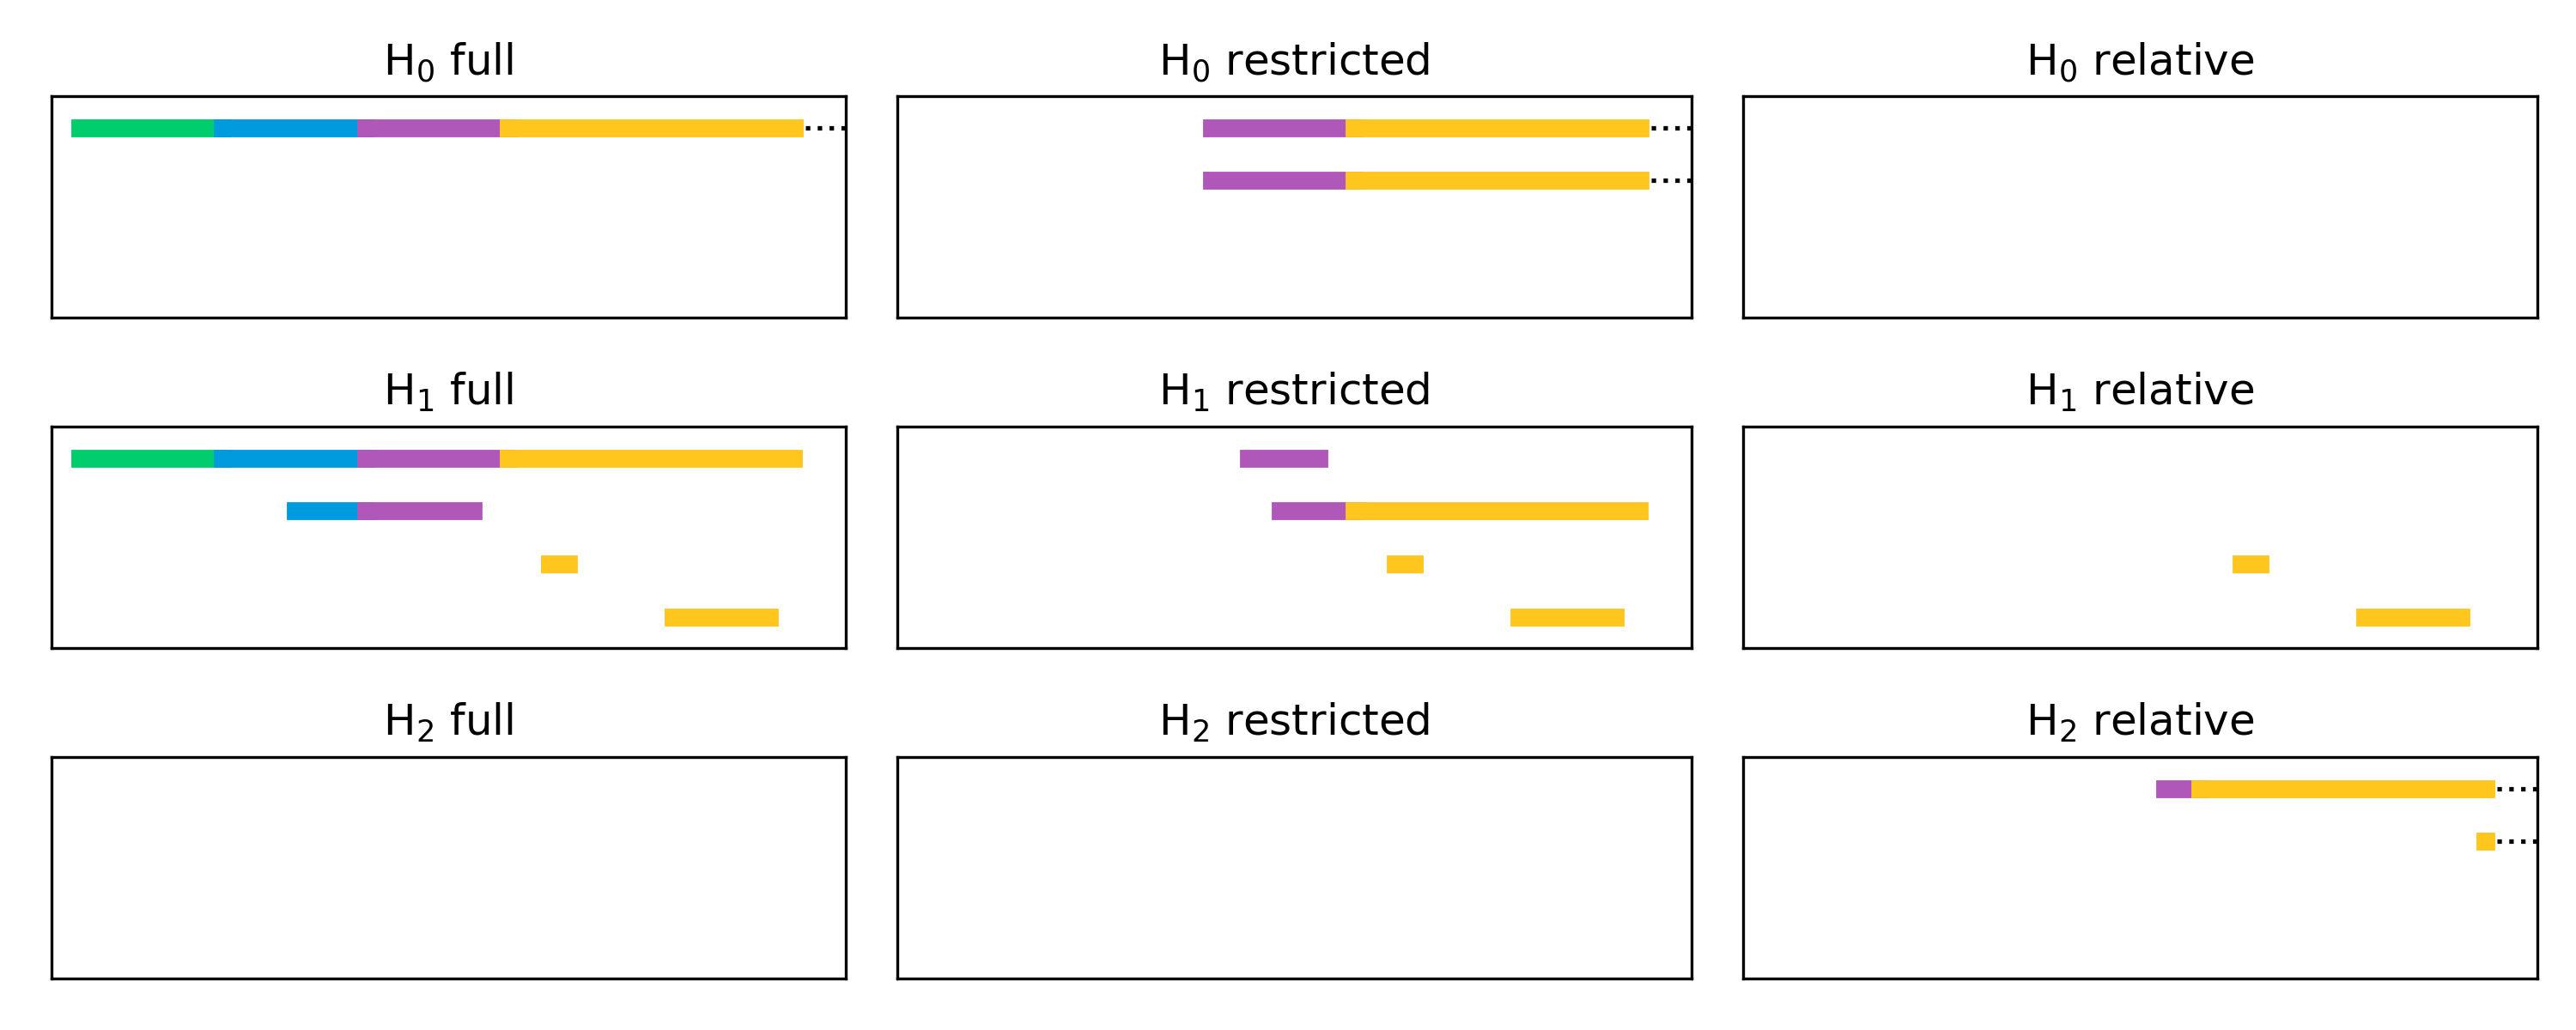
\includegraphics[width=\textwidth]{scripts/figures/barcodes/res_rel.png}
  \end{minipage}
  \caption{Full, restricted, and relative barcodes of the function (left).}
\end{figure}

Let $\LL^k$ denote the $k$th persistent homology module of the sublevel set filtration $\{B_\alpha\}_{\alpha\in\R}$.
As in the previous section, let $\DD{\omega}^k$ denote the $k$th persistent (relative) homology module of $\{(D\subi{\omega}{\alpha}, B_\omega)\}_{\alpha\in\R}$.
Throughout we will assume that we are taking homology in a field $\FF$ and that the homology groups $\hom_k(B_\alpha)$ and $\hom_k(D\subi{\omega}{\alpha}, B_\omega)$ are finite dimensional vector spaces for all $k$ and $\alpha\in\R$.
We will use the interval decomposition of $\LL^k$ to give a decomposition of the relative module $\DD{\omega}^k$ in terms of a \emph{truncation} of $\LL^k$.
For fixed $\omega\in\R$ we will define the truncation $\T^k_\omega$ of $\LL^k$ in terms of the intervals decomposing $\LL^k$ that are in $[\omega, \infty)$.

\paragraph*{Truncated Interval Modules}

For an interval $I = [s,t)\subseteq \R$ let $I_+ := [t,\infty)$ and $I_- := (-\infty, s]$.
For $\omega\in\R$ let $\FF_{\omega}^I$ denote the interval module consisting of vector spaces $\{F\subi{\omega}{\alpha}^I\}_{\alpha\in\R}$ and linear maps $\{f\subi{\omega}{\alpha,\beta}^I : F\subi{\omega}{\alpha}^I\to F\subi{\omega}{\beta}^I\}_{\alpha\leq\beta}$ where
\[ F\subi{\omega}{\alpha}^I := \begin{cases} F_\alpha^I&\text{ if } \omega\in I_-\\ 0&\text{ otherwise,}\end{cases}\ \text{ and }\ \ f\subi{\omega}{\alpha,\beta}^I := \begin{cases} f_{\alpha,\beta}^I&\text{ if } \omega\in I_-\\ 0&\text{ otherwise.}\end{cases}\]
For a collection $\I$ of intervals let $\I_\omega := \{I\in\I\mid \omega\in I\}$.

\begin{lemma}\label{lem:decomposition}
  Suppose $\I^k$ and $\I^{k-1}$ are collections of intervals that decompose $\LL^k$ and $\LL^{k-1}$, respectively.
  Then for all $k$ the $k$th persistent homology module of $\{(D\subi{\omega}{\alpha}, B_\omega)\}_{\alpha\in\R}$ is isomorphic to
  \[\bigoplus_{I\in\I^k} \FF_\omega^I \oplus \bigoplus_{I\in \I_\omega^{k-1}} \FF^{I_+}.\]
\end{lemma}
\begin{proof}
  Suppose $\alpha\leq\omega$.
  So $\hom_k(D\subi{\omega}{\alpha}, B_\omega) = 0$ as $D\subi{\omega}{\alpha} = B_\omega\cup B_\alpha$ and $\T^k_\omega = 0$ as $F_\alpha^I = 0$ for any $I\in \I^k$ such that $\omega\in I_-$.
  Moreover, $\omega\in I$ for all $I\in \I_\omega^{k-1}$, thus $F_\alpha^{I_+} = 0$ for all $\alpha\leq\omega$.
  So it suffices to assume $\omega < \alpha$.

  Consider the long exact sequence of the pair $\hom_k(D\subi{\omega}{\alpha}, B_\omega) = \hom_k(B_\alpha, B_\omega)$
  \[ \ldots\to \hom_k(B_\omega)\xrightarrow{p_\alpha^k} \hom_k(B_\alpha)\xrightarrow{q_\alpha^k}\hom_k(D\subi{\omega}{\alpha}, B_\omega)\xrightarrow{r_\alpha^k} \hom_{k-1}(B_\omega)\xrightarrow{p_\alpha^{k-1}}\hom_{k-1}(B_\alpha)\to\ldots\]
  where $\hom_k(B_\alpha) = \bigoplus_{I\in \I^k}F_\alpha^I$, $\hom_k(B_\omega) = \bigoplus_{I\in \I^k}F_\omega^I$, and $p_\alpha^k = \displaystyle\bigoplus_{I\in\I^k} f_{\omega,\alpha}^I$.

  Noting that $\im~q_\alpha^k \cong \hom_k(B_\alpha) / \ker~q_\alpha^k$ where $\ker~q_\alpha^k = \im~p_\alpha^k$ by exactness we have $\ker~r_\alpha^k \cong \hom_k(B_\alpha) / \im~p_\alpha^k$.
  By the definition of $F_\alpha^I$ and $f_{\omega,\alpha}^I$ we know $\im~f_{\omega,\alpha}^I$ is $F_\alpha^I$ if $\omega\in I$ and 0 otherwise.
  As $\im~p_\alpha^k$ is equal to the direct sum of images $\im~f_{\omega,\alpha}^I$ over $I\in\I^k$ it follows that $\im~p_\alpha^k$ is the direct sum of those $F_\alpha^I$ over those $I\in\I^k$ such that $\omega\in I$.
  Now, because $\hom_k(B_\alpha) = \bigoplus_{I\in \I^k}F_\alpha^I$ and each $F_\alpha^I$ is either 0 or $\FF$ the quotient $\hom_k(B_\alpha) / \im~p_\alpha^k$ is the direct sum of those $F_\alpha^I$ such that $\omega\notin I$.
  Therefore, by the definition of $F\subi{\omega}{\alpha}^I$ we have
  \[ \ker~r_\alpha^k = \bigoplus_{I\in\I_\omega^k} F\subi{\omega}{\alpha}^I.\]

  Similarly, $\im~r_\alpha^k = \ker~p_\alpha^{k-1}$ by exactness where $\ker~p_\alpha^{k-1}$ is the direct sum of kernels $\ker~f_{\omega,\alpha}^I$ over $I\in\I^{k-1}$.
  By the definition of $F_\alpha^I$ and $f_{\omega,\alpha}^I$ we know that $\ker~f_{\omega,\alpha}^I$ is $F_\alpha^I$ if $\omega\notin I$ and $0$ otherwise.
  Noting that $\ker~f_{\omega,\alpha}^I = 0$ for any $I\in \I^{k-1}$ such that $\omega\notin I$ it suffices to consider only those $I\in \I_\omega^{k-1}$.
  It follows that $\ker~f_{\omega,\alpha}^I = F_\alpha^{I_+}$ for any $I$ containing $\omega$ as $\omega < \alpha$.
  Therefore,
  \[\im~r_\alpha^k = \bigoplus_{I\in\I^{k-1}} F_\alpha^{I_+}.\]

  We have the following split exact sequence associated with $r_\alpha^k$
  \[ 0\to \ker~r_\alpha^k\to \hom_k(D\subi{\omega}{\alpha}, B_\omega)\to\im~r_\alpha^k\to 0.\]
  The desired result follows from the fact that for all $\alpha\in\R$
  \begin{align*}
    \hom_k(D\subi{\omega}{\alpha}, B_\omega) &\cong \ker~r_\alpha^k\oplus \im~r_\alpha^k =\bigoplus_{I\in\I^k} F\subi{\omega}{\alpha}^I\oplus \bigoplus_{I\in\I_\omega^{k-1}} F_\alpha^{I_+}.
  \end{align*}
\end{proof}

Letting $\I^k$ denote the decomposing intervals of $\LL^k$ for all $k$ we can define the \textbf{$\omega$-truncated $k$th persistent homology module} of $\LL^k$ as
\[ \T_\omega^k := \bigoplus_{I\in\I^k} \FF_\omega^I\ \text{ and let }\ \LL_\omega^{k-1} := \bigoplus_{I\in \I_\omega^{k-1}} \FF^{I_+}\]
denote the submodule of $\DD{\omega}^k$ consisting of intervals $[\beta,\infty)$ corresponding to features $[\alpha,\beta)$ in $\LL^{k-1}$ such that $\alpha\leq\omega <\beta$.
Now, by Lemma~\ref{lem:decomposition} the $k$th persistent (relative) homology module of $\{(D\subi{\omega}{\alpha}, B_\omega)\}_{\alpha\in\R}$ is $\DD{\omega}^k = \T_\omega^k\oplus \LL_\omega^{k-1}.$
Theorems~\ref{thm:algo_tcc} and~\ref{thm:interleaving_main_2} can then be used to show that
\[ \{\rips^{2\delta}(P\subi{\omega-2c\delta}{\alpha}, Q_{\omega-2c\delta})\hookrightarrow \rips^{4\delta}(P\subi{\omega+c\delta}{\alpha}, Q_{\omega+c\delta})\}_{\alpha\in\R} \]
is $4c\delta$ interleaved with $\T_\omega^k\oplus \LL_\omega^{k-1}$ whenever
\[ \rk~\hom_d(\rips^\delta(P, Q_{\omega - 2c\delta})\hookrightarrow \rips^{2\delta}(P, Q_{\omega+c\delta})) \geq \dim~\hom_0(\rips^\delta(P\setminus Q_{\omega-2c\delta})).\]


%   If $\rk~\hom_d(\rips^\delta(P, Q_{\omega - 2c\delta})\hookrightarrow \rips^{2\delta}(P, Q_{\omega+c\delta})) \geq \dim~\hom_0(\rips^\delta(P\setminus Q_{\omega-2c\delta}))$ then the $k$th (relative) homology module of $\{\rips^{2\delta}(P\subi{\omega-2c\delta}{\alpha}, Q_{\omega-2c\delta})\hookrightarrow \rips^{4\delta}(P\subi{\omega+c\delta}{\alpha}, Q_{\omega+c\delta})\}_{\alpha\in\R}$ is $4c\delta$-interleaved with $\T_{\omega}^k \oplus \LL_\omega^{k-1}$: the $k$th persistent homology module of $\{(D\subi{\omega}{\alpha}, B_\omega)\}_{\alpha\in\R}$.
%
% Our main theorem combines this decomposition with our coverage and interleaving results of Theorems~\ref{thm:algo_tcc} and~\ref{thm:interleaving_main_2}.% as a method for certified approximation of the truncated persistence diagram.\textbf{TODO: GROSS}

% \begin{lemma}\label{lem:dual_ass}
%   Let $\X$ be an orientable $d$-manifold and suppose $(D, B)$ and $(D, B')$ are compact, locally contractible, surrounding pairs in $\X$ such that $\hom_d(D, B)$ and $\hom_d(D, B')$ are finitely generated.
%
%   If $\hom_{d-1}(B\hookrightarrow B')$ is surjective then $\hom_0(D\setminus B'\hookrightarrow D\setminus B)$ is injective.
%   If $\hom_{d-1}(B\hookrightarrow B')$ is injective then $\hom_0(D\setminus B'\hookrightarrow D\setminus B)$ is surjective.
% \end{lemma}
% \begin{proof}
%   If $\hom_{d-1}(B\hookrightarrow B')$ is surjective for all $k$ then $\hom_d((D, B)\hookrightarrow (D, B'))$ is surjective by the five lemma.
%   Taking homology with coefficients in a field $\FF$ we can dualize to obtain an \emph{injective} map $\Hom(\hom_d(D,B'), \FF)\to \Hom(\hom_d(D, B), \FF)$.
%   Therefore, because we are taking coefficients in a field, we have an injective map $\hom^d(D,B')\to \hom^d(D, B)$ by the Universal Coefficient Theorem.
%
%   Because $(D, B)$ and $(D,B')$ are compact and locally connected we can apply Alexander Duality to obtain an injective map $\hom_0(\X\setminus B', \X\setminus D)\to\hom_0(\X\setminus B, \X\setminus D)$.
%   Because $B,B'$ surround $D$ in $\X$ it follows that $\hom_0(D\setminus B'\hookrightarrow D\setminus B)$ is injective.
%   It can be shown $\hom_{d-1}(B\hookrightarrow B')$ injective implies $\hom_0(D\setminus B'\hookrightarrow D\setminus B)$ surjective by a similar argument.
% \end{proof}
%
% \begin{theorem}\label{thm:main}
%   Let $\X$ be an orientable $d$-manifold and let $D$ be a compact subset of $\X$.
%   Let $f : D\to\R$ be a $c$-Lipschitz function and $\omega\in\R$, $\delta < \varrho_D/4$ be constants such that $P\subset D$ is a $(\delta, 2\delta,\omega)$-sublevel sample of $f$ and $B_{\omega-3c\delta}$ surrounds $D$ in $\X$.
%   % Let $P$ be a finite subset of $D$ such that $(P, Q_{\omega-2c\delta})$ and $(P, Q_{\omega+c\delta})$ are $\delta$-good samples of $(D, B_\omega)$.
%   % Let $P\subset \intr_\X(D)$ and suppose $D\setminus P^\delta$, $D\setminus Q_{\omega-2c\delta}^\delta$, and $D\setminus Q_{\omega+c\delta}^\delta$ are locally path connected.
%
%   Suppose $\hom_k(B_{\omega-3c\delta}\hookrightarrow B_\omega)$ is surjective and $\hom_k(B_\omega\hookrightarrow B_{\omega+5c\delta})$ is an isomorphism for all $k$.
%   If $\rk~\hom_d(\rips^\delta(P, Q_{\omega - 2c\delta})\hookrightarrow \rips^{2\delta}(P, Q_{\omega+c\delta})) \geq \dim~\hom_0(\rips^\delta(P\setminus Q_{\omega-2c\delta}))$ then the $k$th (relative) homology module of $\{\rips^{2\delta}(P\subi{\omega-2c\delta}{\alpha}, Q_{\omega-2c\delta})\hookrightarrow \rips^{4\delta}(P\subi{\omega+c\delta}{\alpha}, Q_{\omega+c\delta})\}_{\alpha\in\R}$ is $4c\delta$-interleaved with $\T_{\omega}^k \oplus \LL_\omega^{k-1}$: the $k$th persistent homology module of $\{(D\subi{\omega}{\alpha}, B_\omega)\}_{\alpha\in\R}$.
%    % that of $\{(D\subi{\omega}{\alpha}, B_\omega)\}_{\alpha\in\R}$.
% \end{theorem}
% \begin{proof}
%   If $\hom_k(B_{\omega-3c\delta}\hookrightarrow B_\omega)$ is surjective for all $k$ then, in particular, $\hom_{d-1}(B_{\omega-3c\delta}\hookrightarrow B_\omega)$ is surjective.
%   If $\hom_k(B_{\omega-3c\delta}\hookrightarrow B_\omega)$ is surjective for all $k$ then, in particular, $\hom_{d-1}(B_{\omega-3c\delta}\hookrightarrow B_\omega)$ is surjective.
%   Because $B_{\omega-3c\delta}, B_\omega$ are closed in $D$, and $D$ is compact, $(D, B_{\omega-3c\delta})$ and $(D,B_\omega)$ are compact pairs.
%   If our pairs are locally contractible then $\hom_0(D\setminus B_\omega\hookrightarrow D\setminus B_{\omega-3c\delta})$ is injective and $\hom_0(D\setminus B_{\omega-5c\delta}\hookrightarrow D\setminus B_\omega)$ is surjective by Lemma~\ref{lem:dual_ass}.
%
%   Because $\rk~\hom_d(\rips^\delta(P, Q_{\omega - 2c\delta})\hookrightarrow \rips^{2\delta}(P, Q_{\omega+c\delta})) \geq \dim~\hom_0(\rips^\delta(P\setminus Q_{\omega-2c\delta}))$ and $P\subset D$ is a $(\delta, 2\delta,\omega)$-sublevel sample of $f$ we have $D\setminus B_\omega\subseteq P^\delta$ and $Q_{\omega-2c\delta}^\delta$ surrounds $P^\delta$ in $D$ by Theorem~\ref{thm:algo_tcc}.
%   So the persistent homology modules of $\{\rips^{2\delta}(P\subi{\omega-2c\delta}{\alpha}, Q_{\omega-2c\delta})\hookrightarrow \rips^{4\delta}(P\subi{\omega+c\delta}{\alpha}, Q_{\omega+c\delta})\}_{\alpha\in\R}$ are $4c\delta$ interleaved with those of $\{(D\subi{\omega}{\alpha}, B_\omega)\}_{\alpha\in\R}$ by Theorem~\ref{thm:interleaving_main_2}, and therefore $\T_{\omega}^k \oplus \LL_\omega^{k-1}$ by Lemma~\ref{lem:decomposition}.
% \end{proof}
 % 43

\section{Experiments}\label{sec:experiments}
% % !TeX root = ../../main.tex

\begin{figure}[htbp]\label{fig:ripple1}
  \centering
  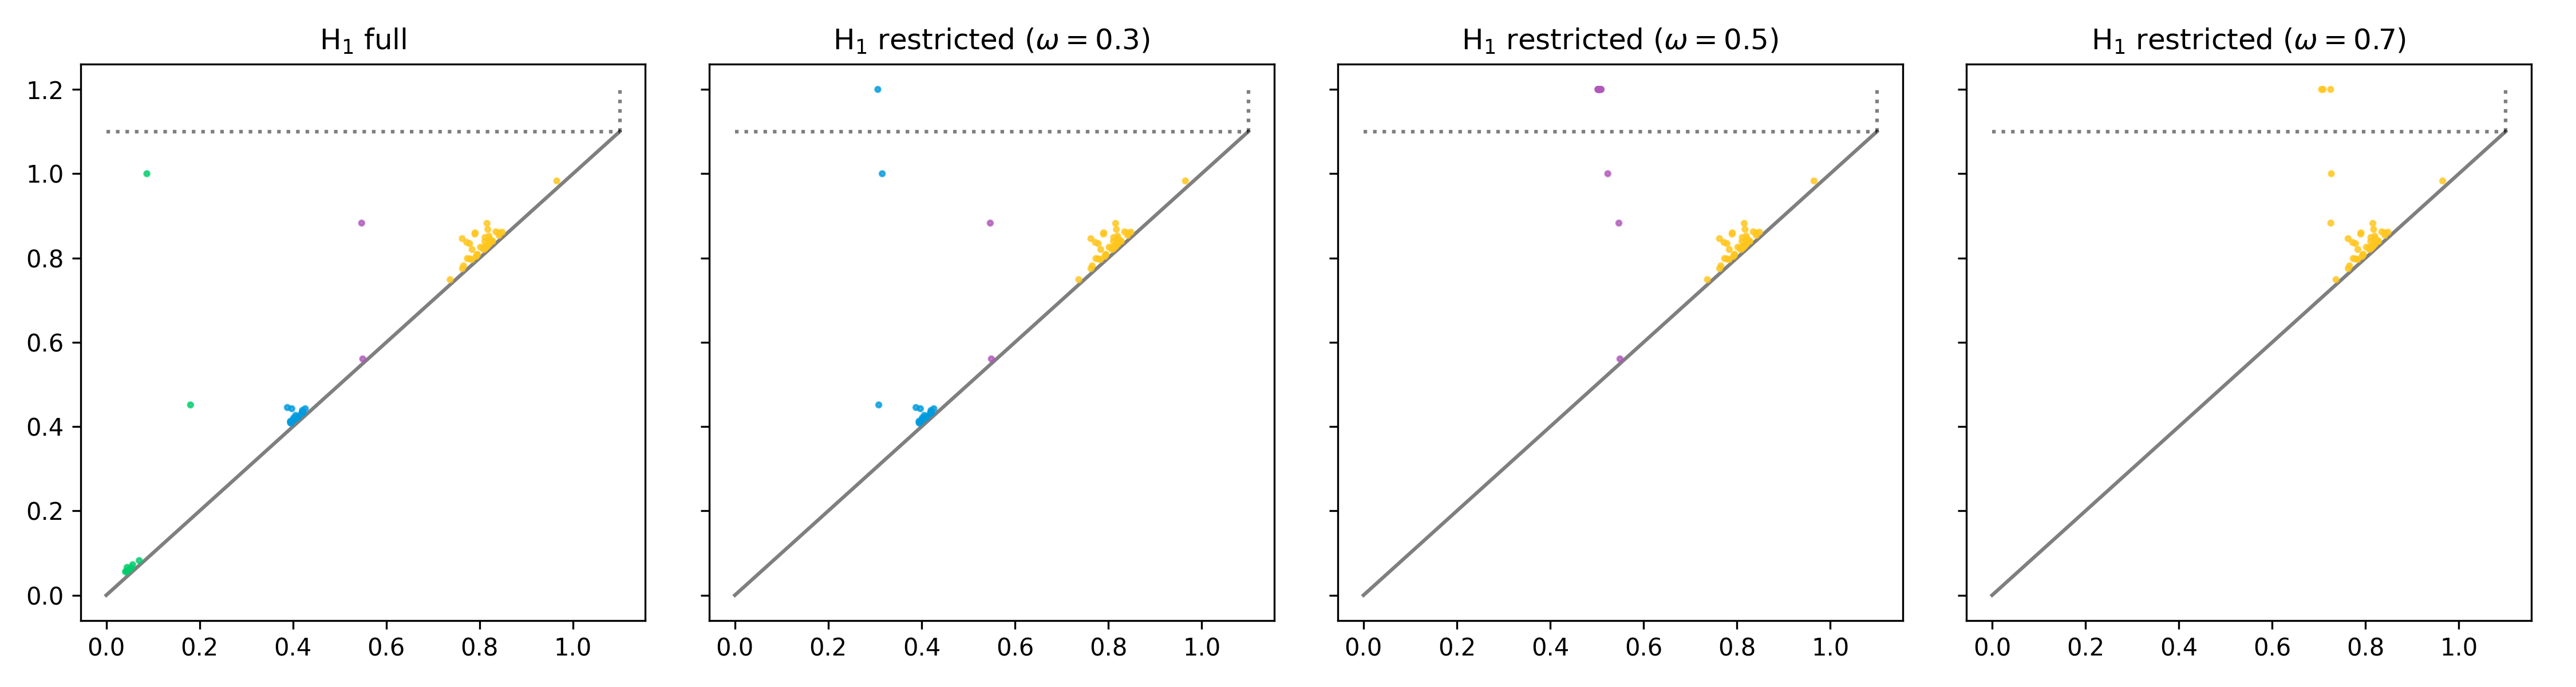
\includegraphics[trim=0 0 790 0, clip, width=0.3\textwidth]{scripts/figures/matching2/full-dgm.png}
  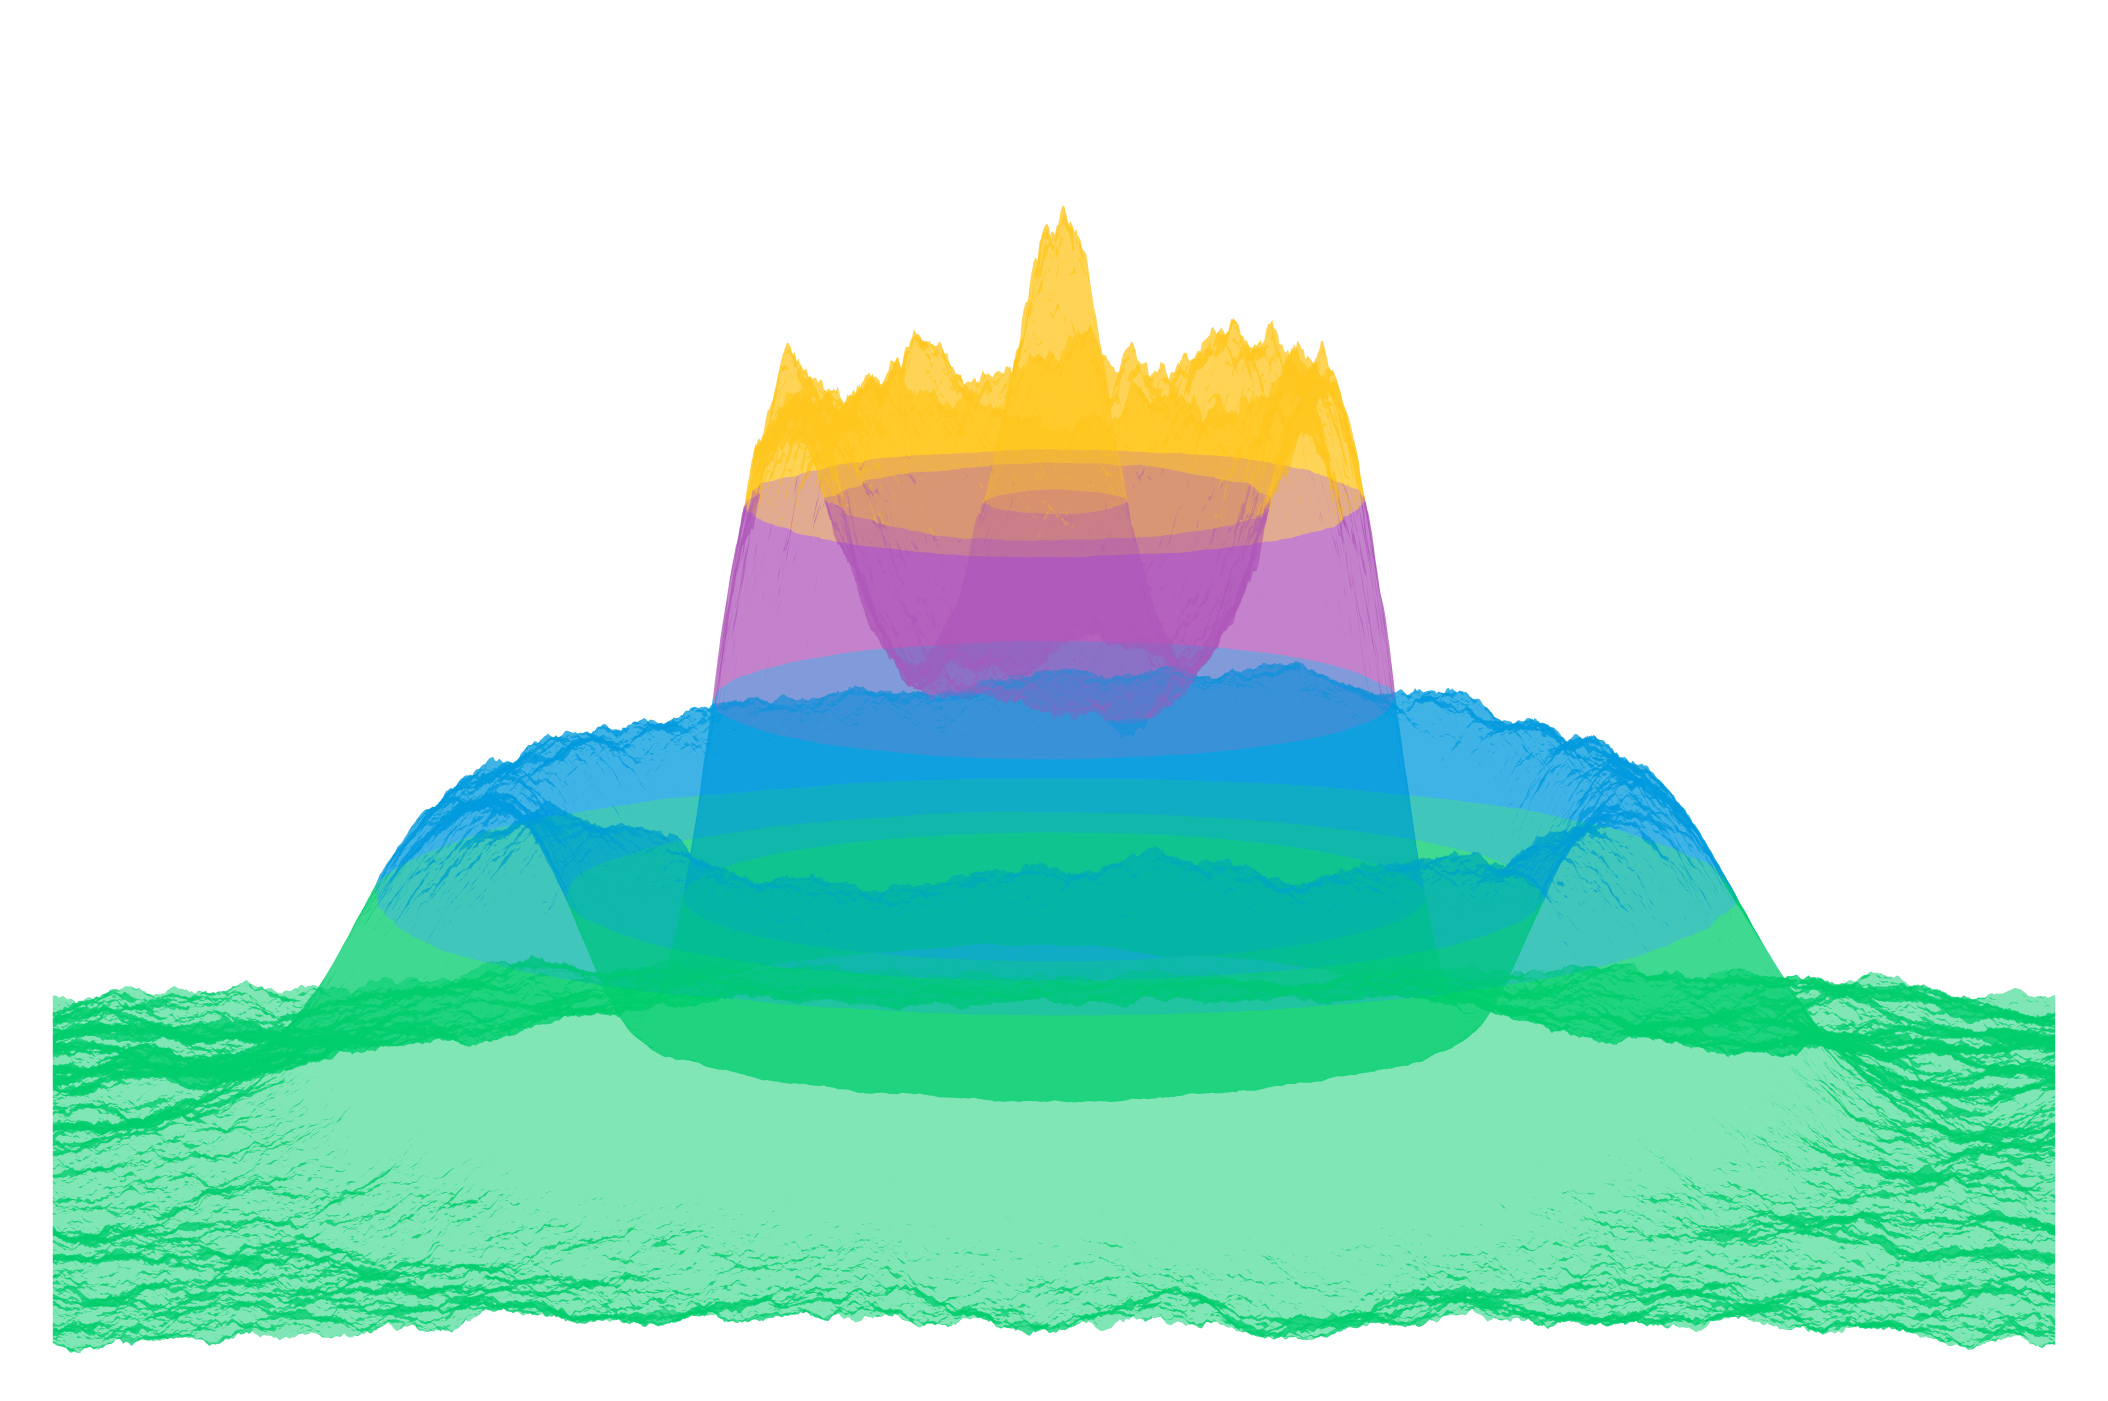
\includegraphics[trim=-350 -800 -700 -300, clip, width=0.4\textwidth]{scripts/figures/matching2/full-surf_side-lowres.png}
  
\includegraphics[trim=0 -800 0 0, width=0.25\textwidth]{scripts/figures/matching2/full-surf_top-lowres.png}
  % \includegraphics[trim=0 0 0 -10, clip, width=\textwidth]{scripts/figures/matching1/817_1024-3_1-1_1.png}
  \caption{The $\hom_1$ persistence diagram of the sinusoidal function pictured to the right.
          Features are colored by birth time, infinite features are drawn above the dotted line.}
\end{figure}

\begin{figure}[htbp]
  \centering
  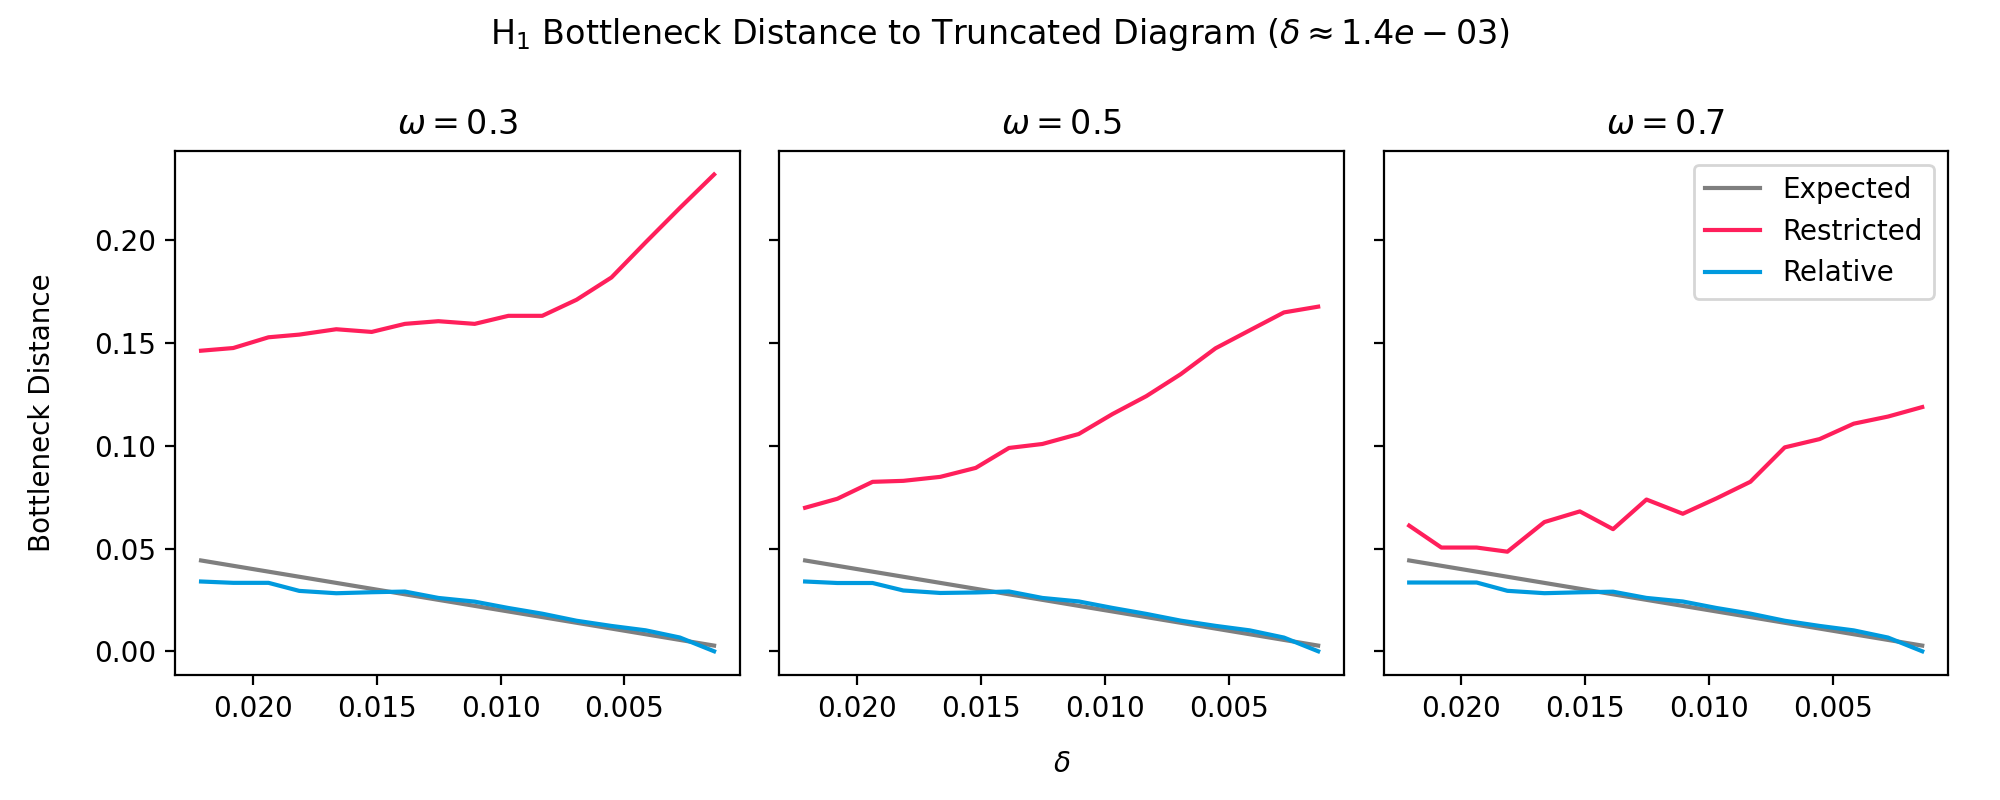
\includegraphics[width=\textwidth]{scripts/figures/matching2/bottleneck_delta.png}
  \caption{Comparison of the bottleneck distance between the truncated diagram of the function shown in Figure~\ref{fig:ripple1} approximated with $\delta\approx 1.4\times10^{-3}$ ($1024\times 1024$ grid) and those of the restricted and relative diagrams with decreasing $\delta$ (increasing grid size 64-1024).}
\end{figure}

\begin{figure}[htbp]
  \centering
  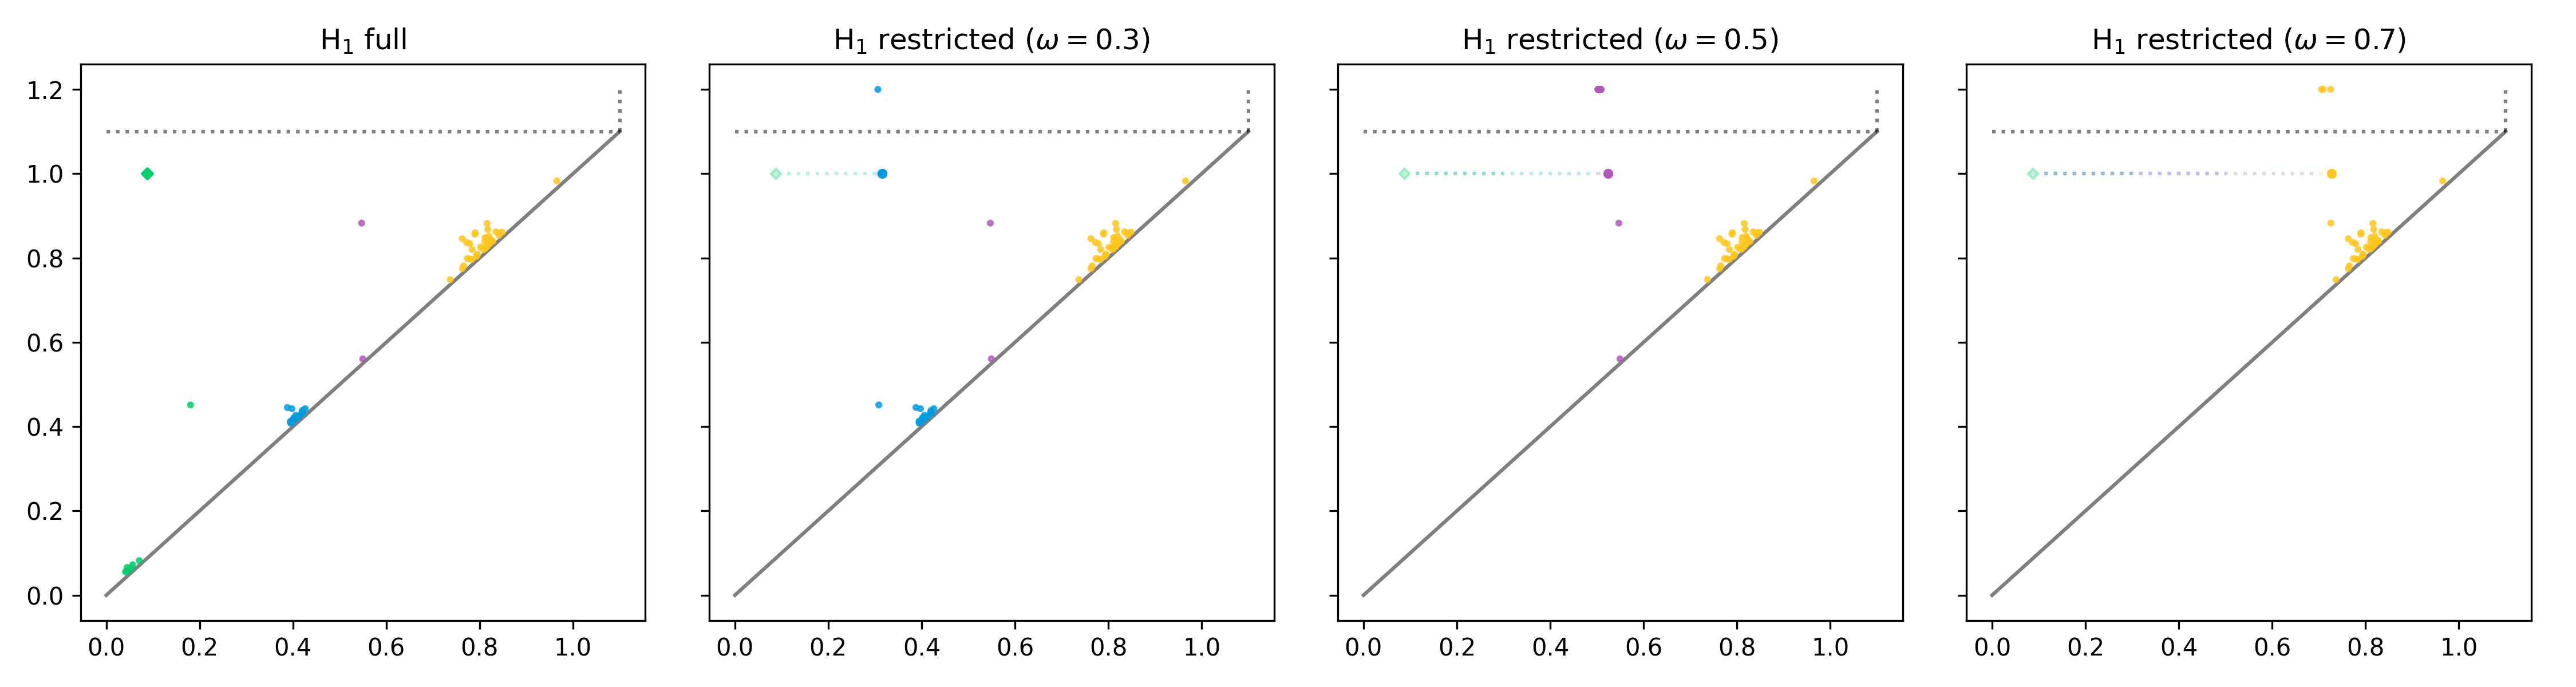
\includegraphics[trim=0 0 -10 0, clip, width=\textwidth]{scripts/figures/matching2/dgm-1.png}
  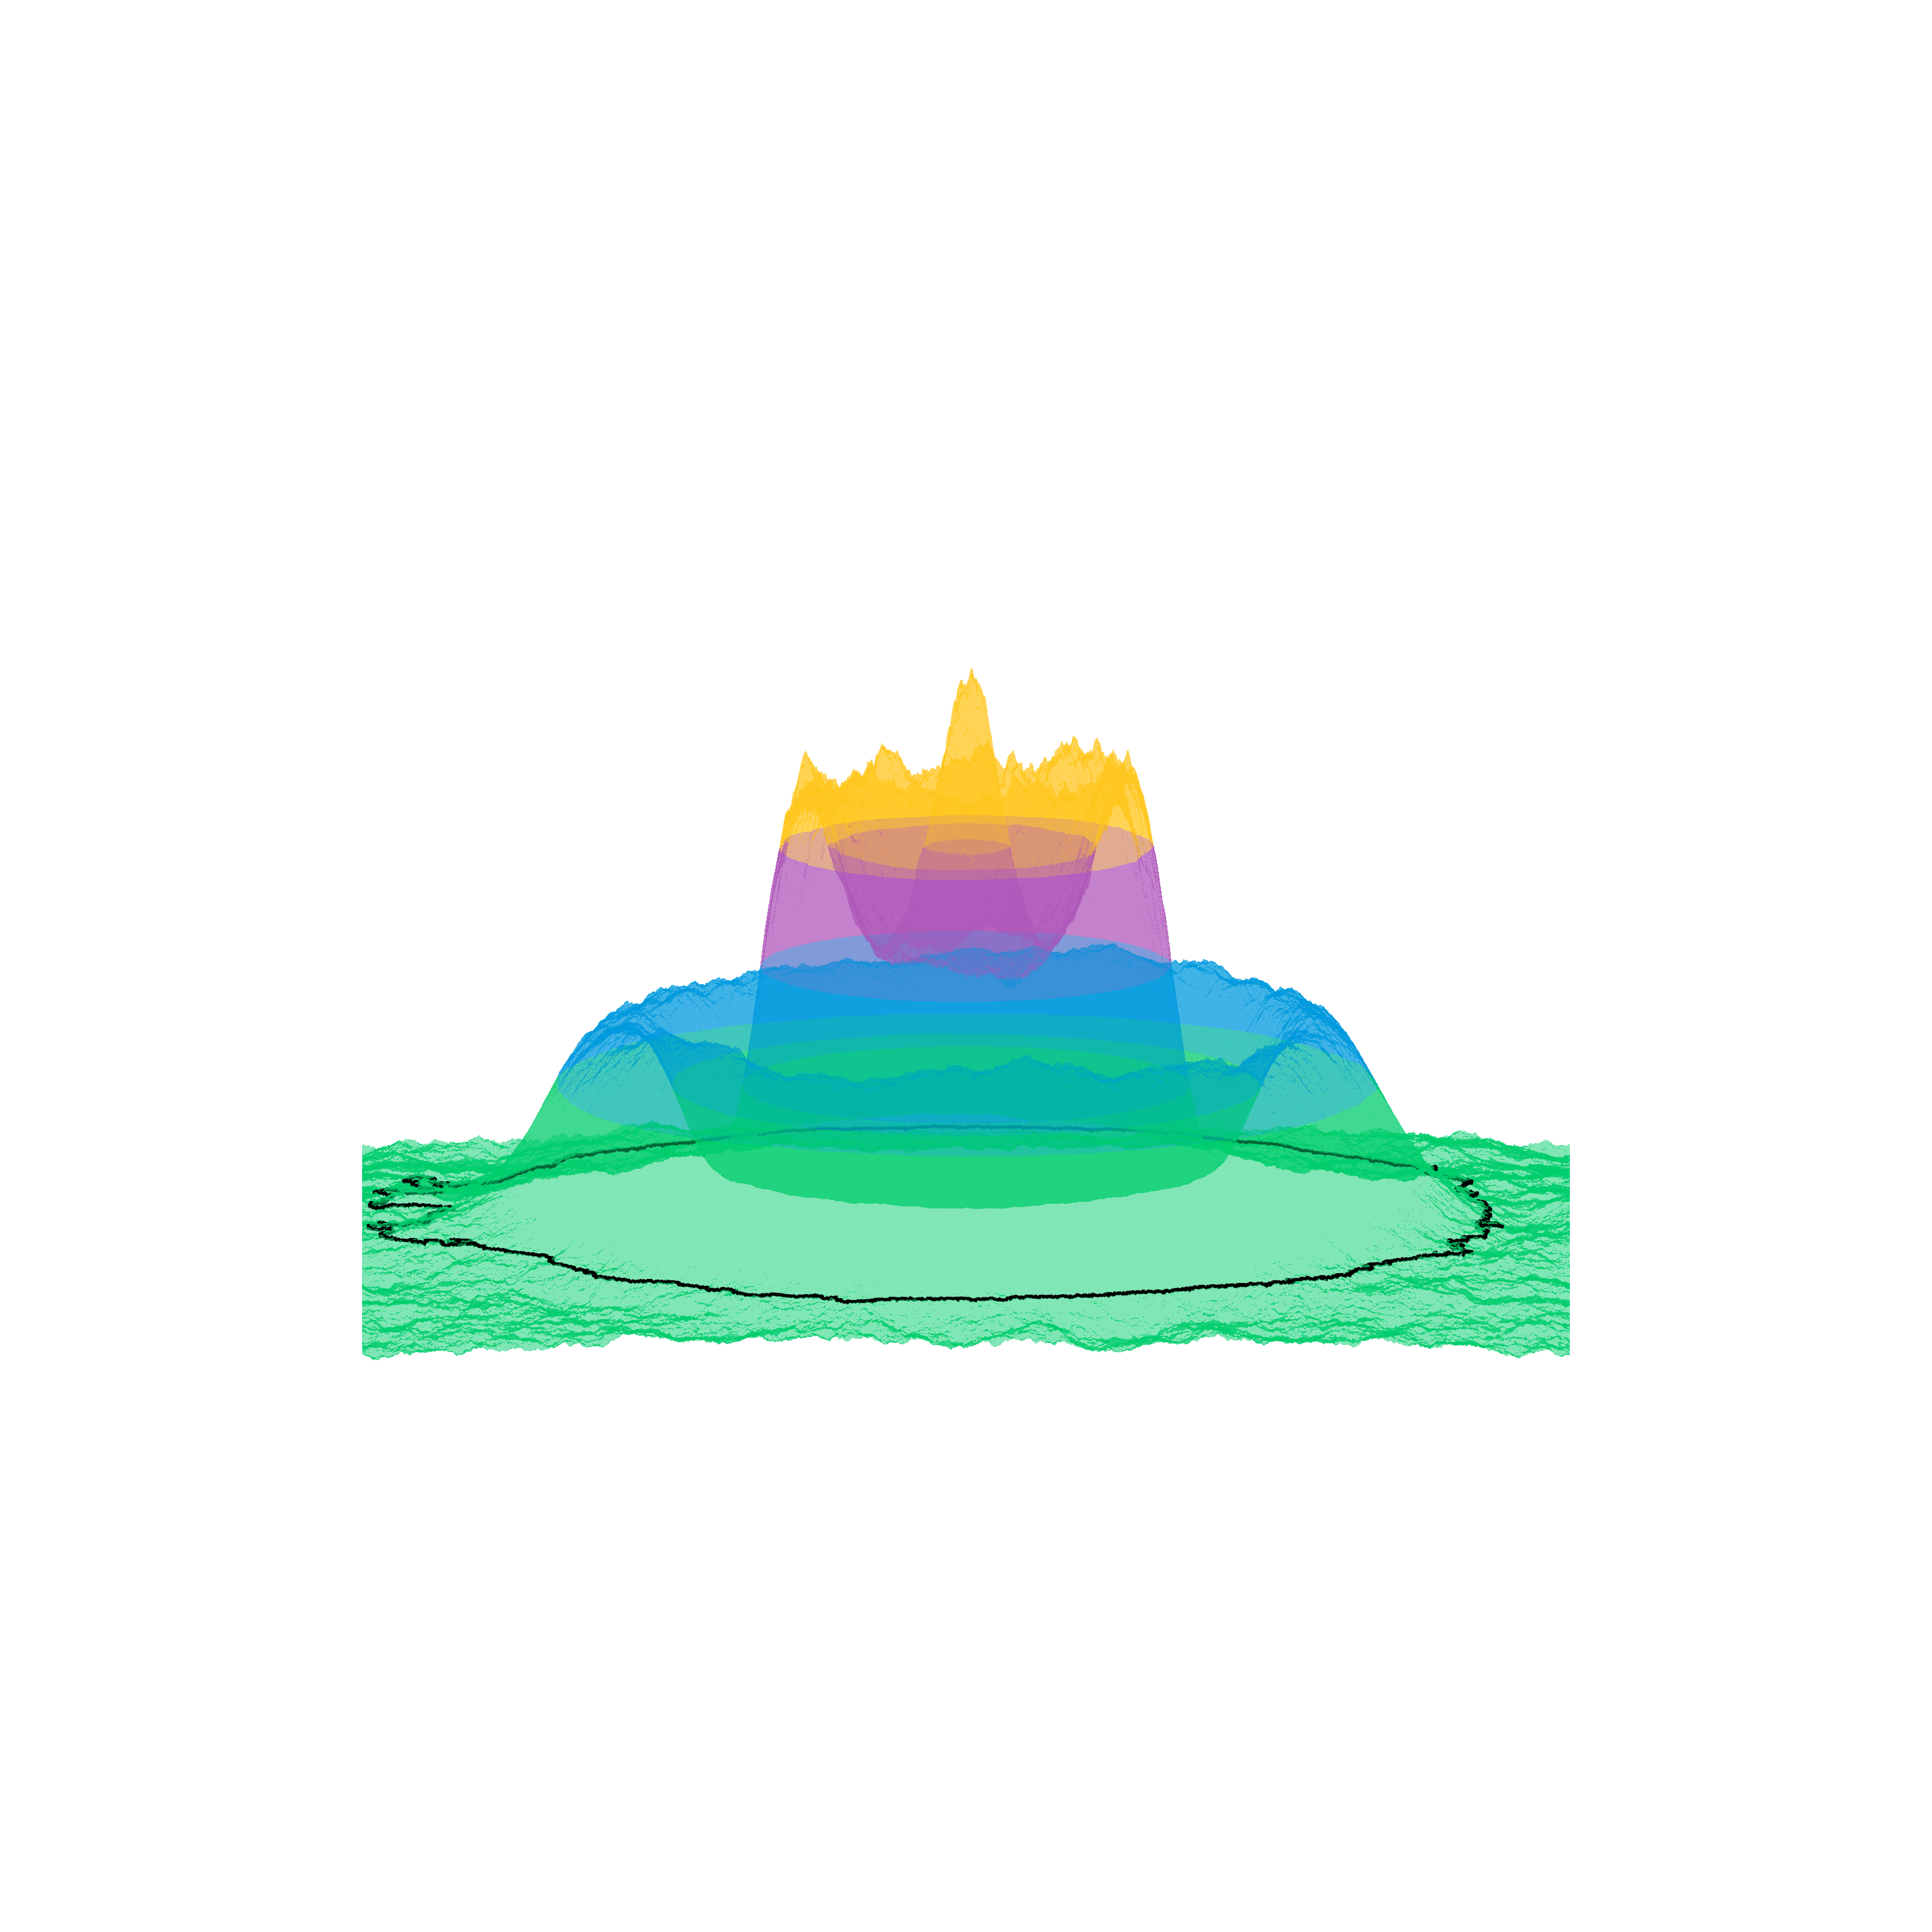
\includegraphics[trim=500 800 500 800, clip, width=0.24\textwidth]{scripts/figures/matching2/surf_side-1.png}
  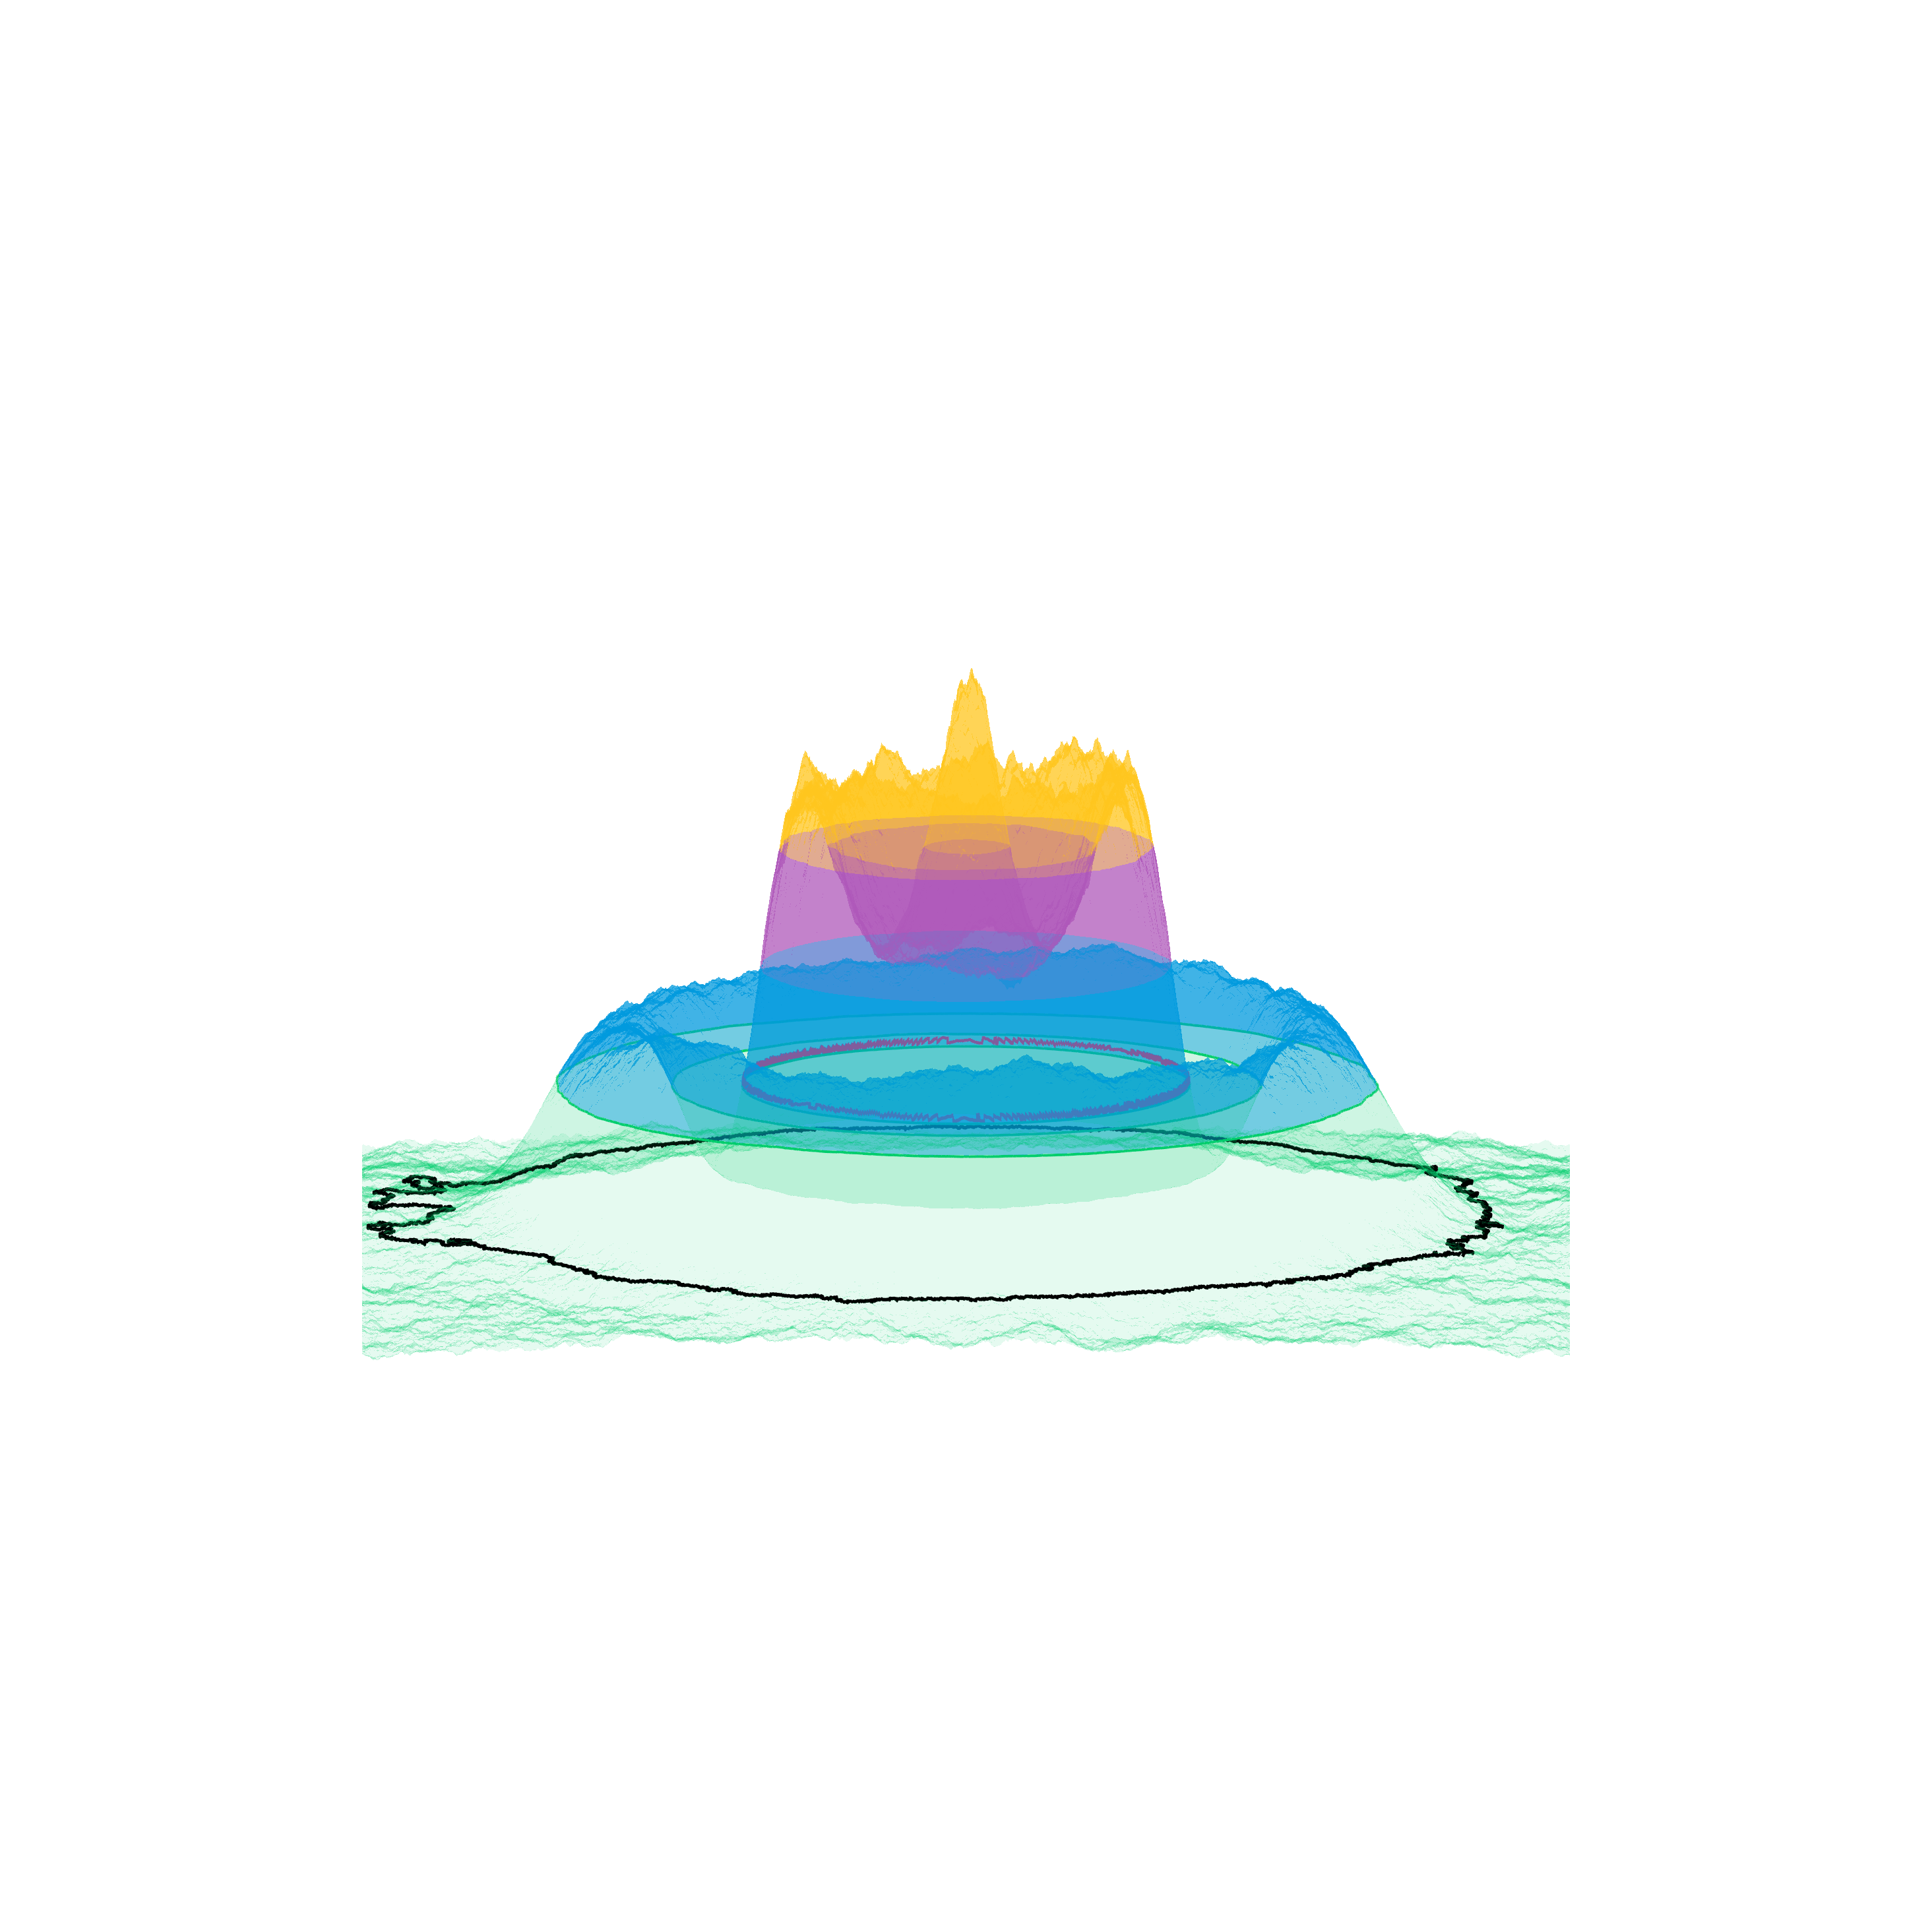
\includegraphics[trim=500 800 500 800, clip, width=0.24\textwidth]{scripts/figures/matching2/surf_side-1_0.png}
  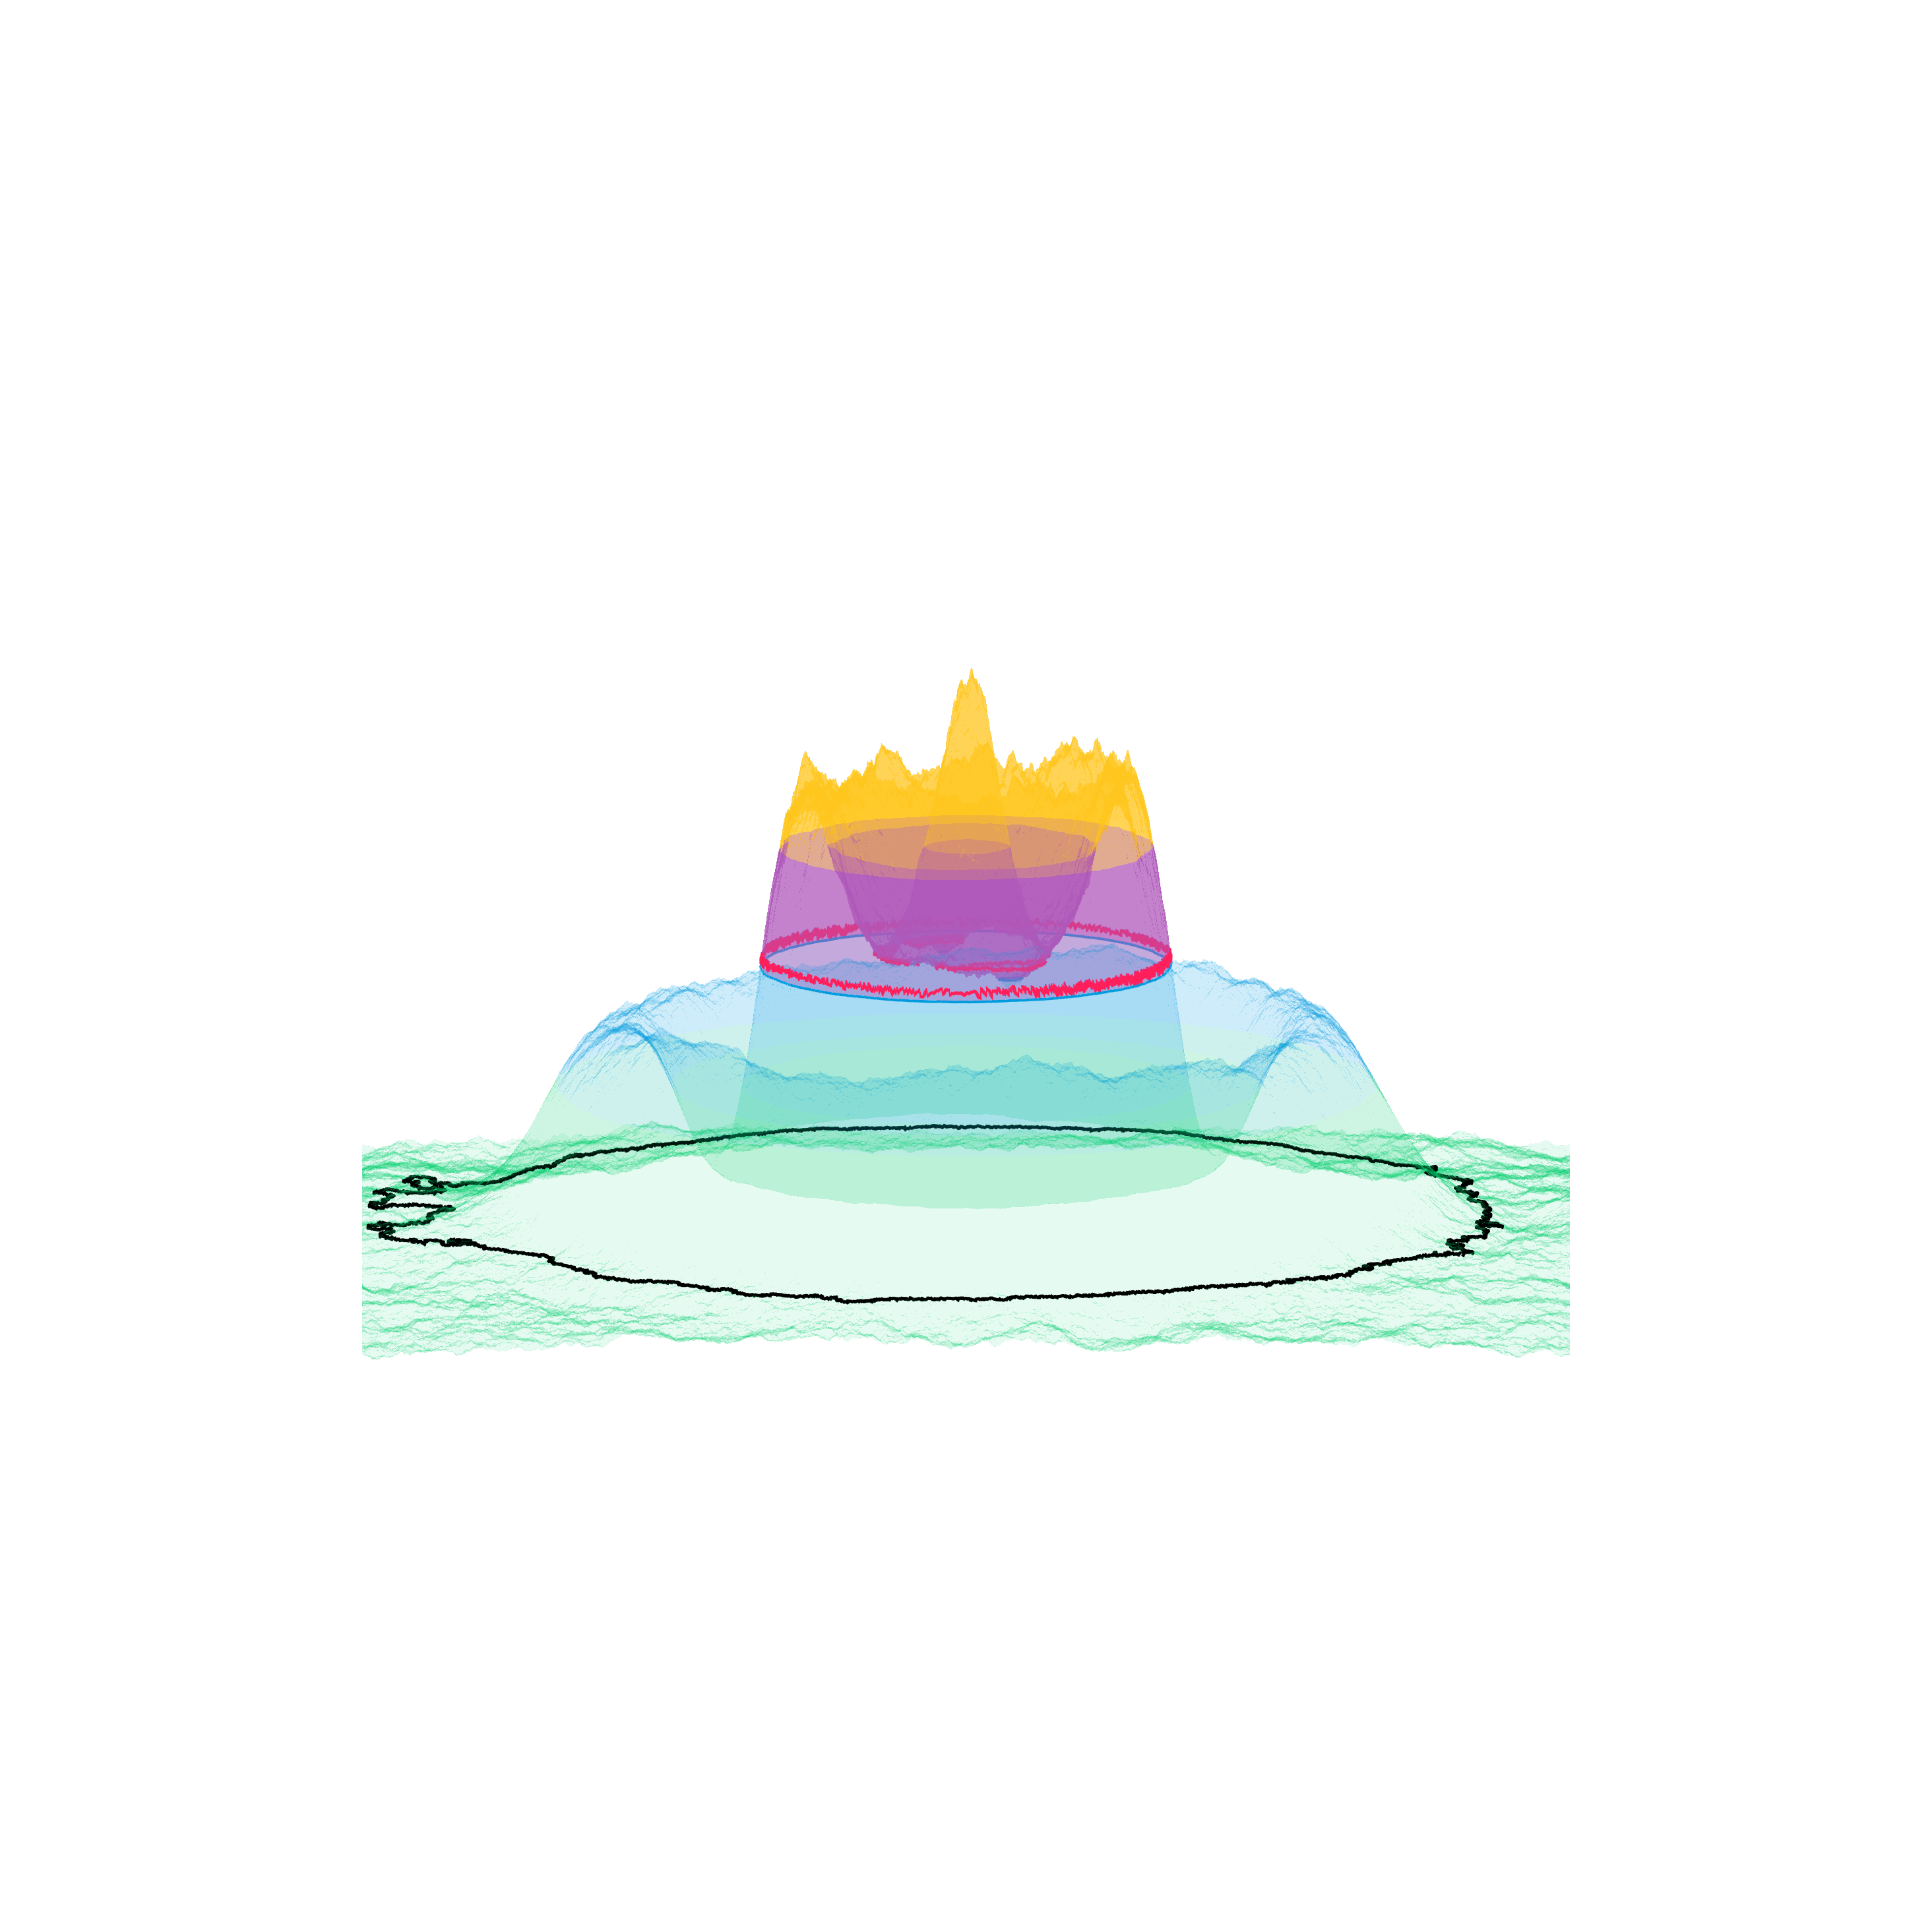
\includegraphics[trim=500 800 500 800, clip, width=0.24\textwidth]{scripts/figures/matching2/surf_side-1_1.png}
  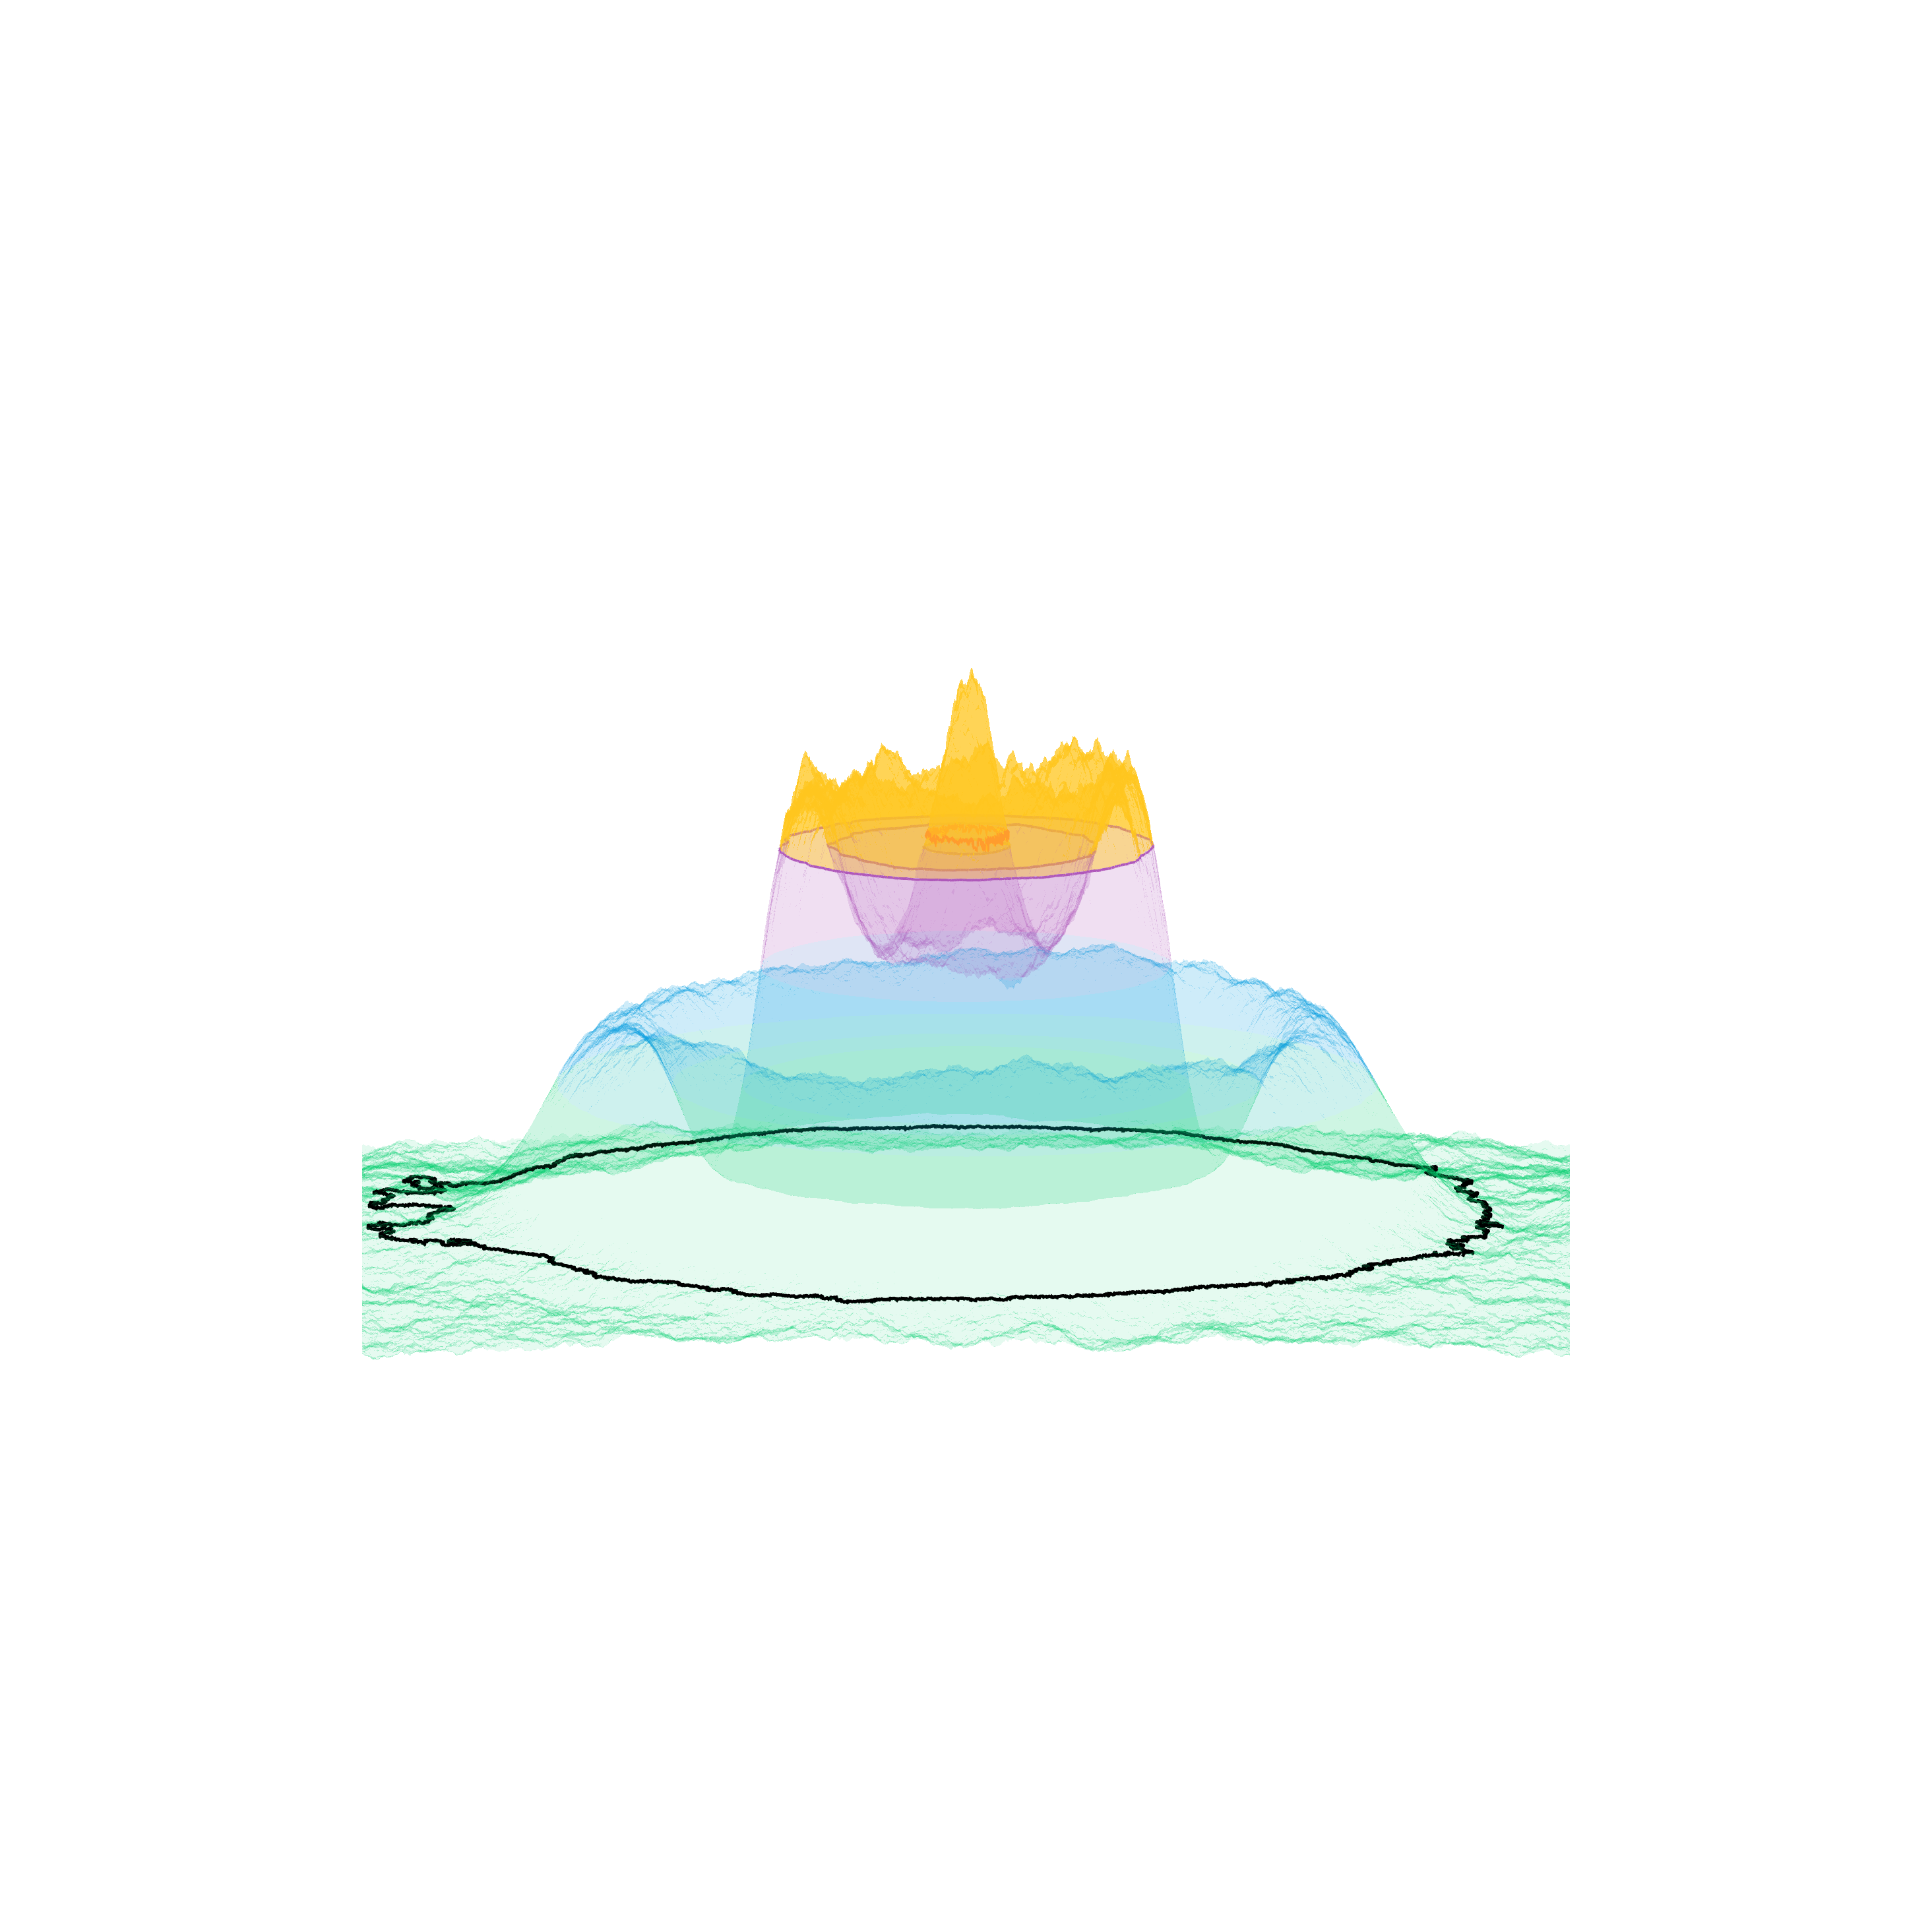
\includegraphics[trim=500 800 500 800, clip, width=0.24\textwidth]{scripts/figures/matching2/surf_side-1_2.png}
  
\includegraphics[trim=500 500 500 500, clip, width=0.24\textwidth]{scripts/figures/matching2/surf_top-1.png}
  
\includegraphics[trim=500 500 500 500, clip, width=0.24\textwidth]{scripts/figures/matching2/surf_top-1_0.png}
  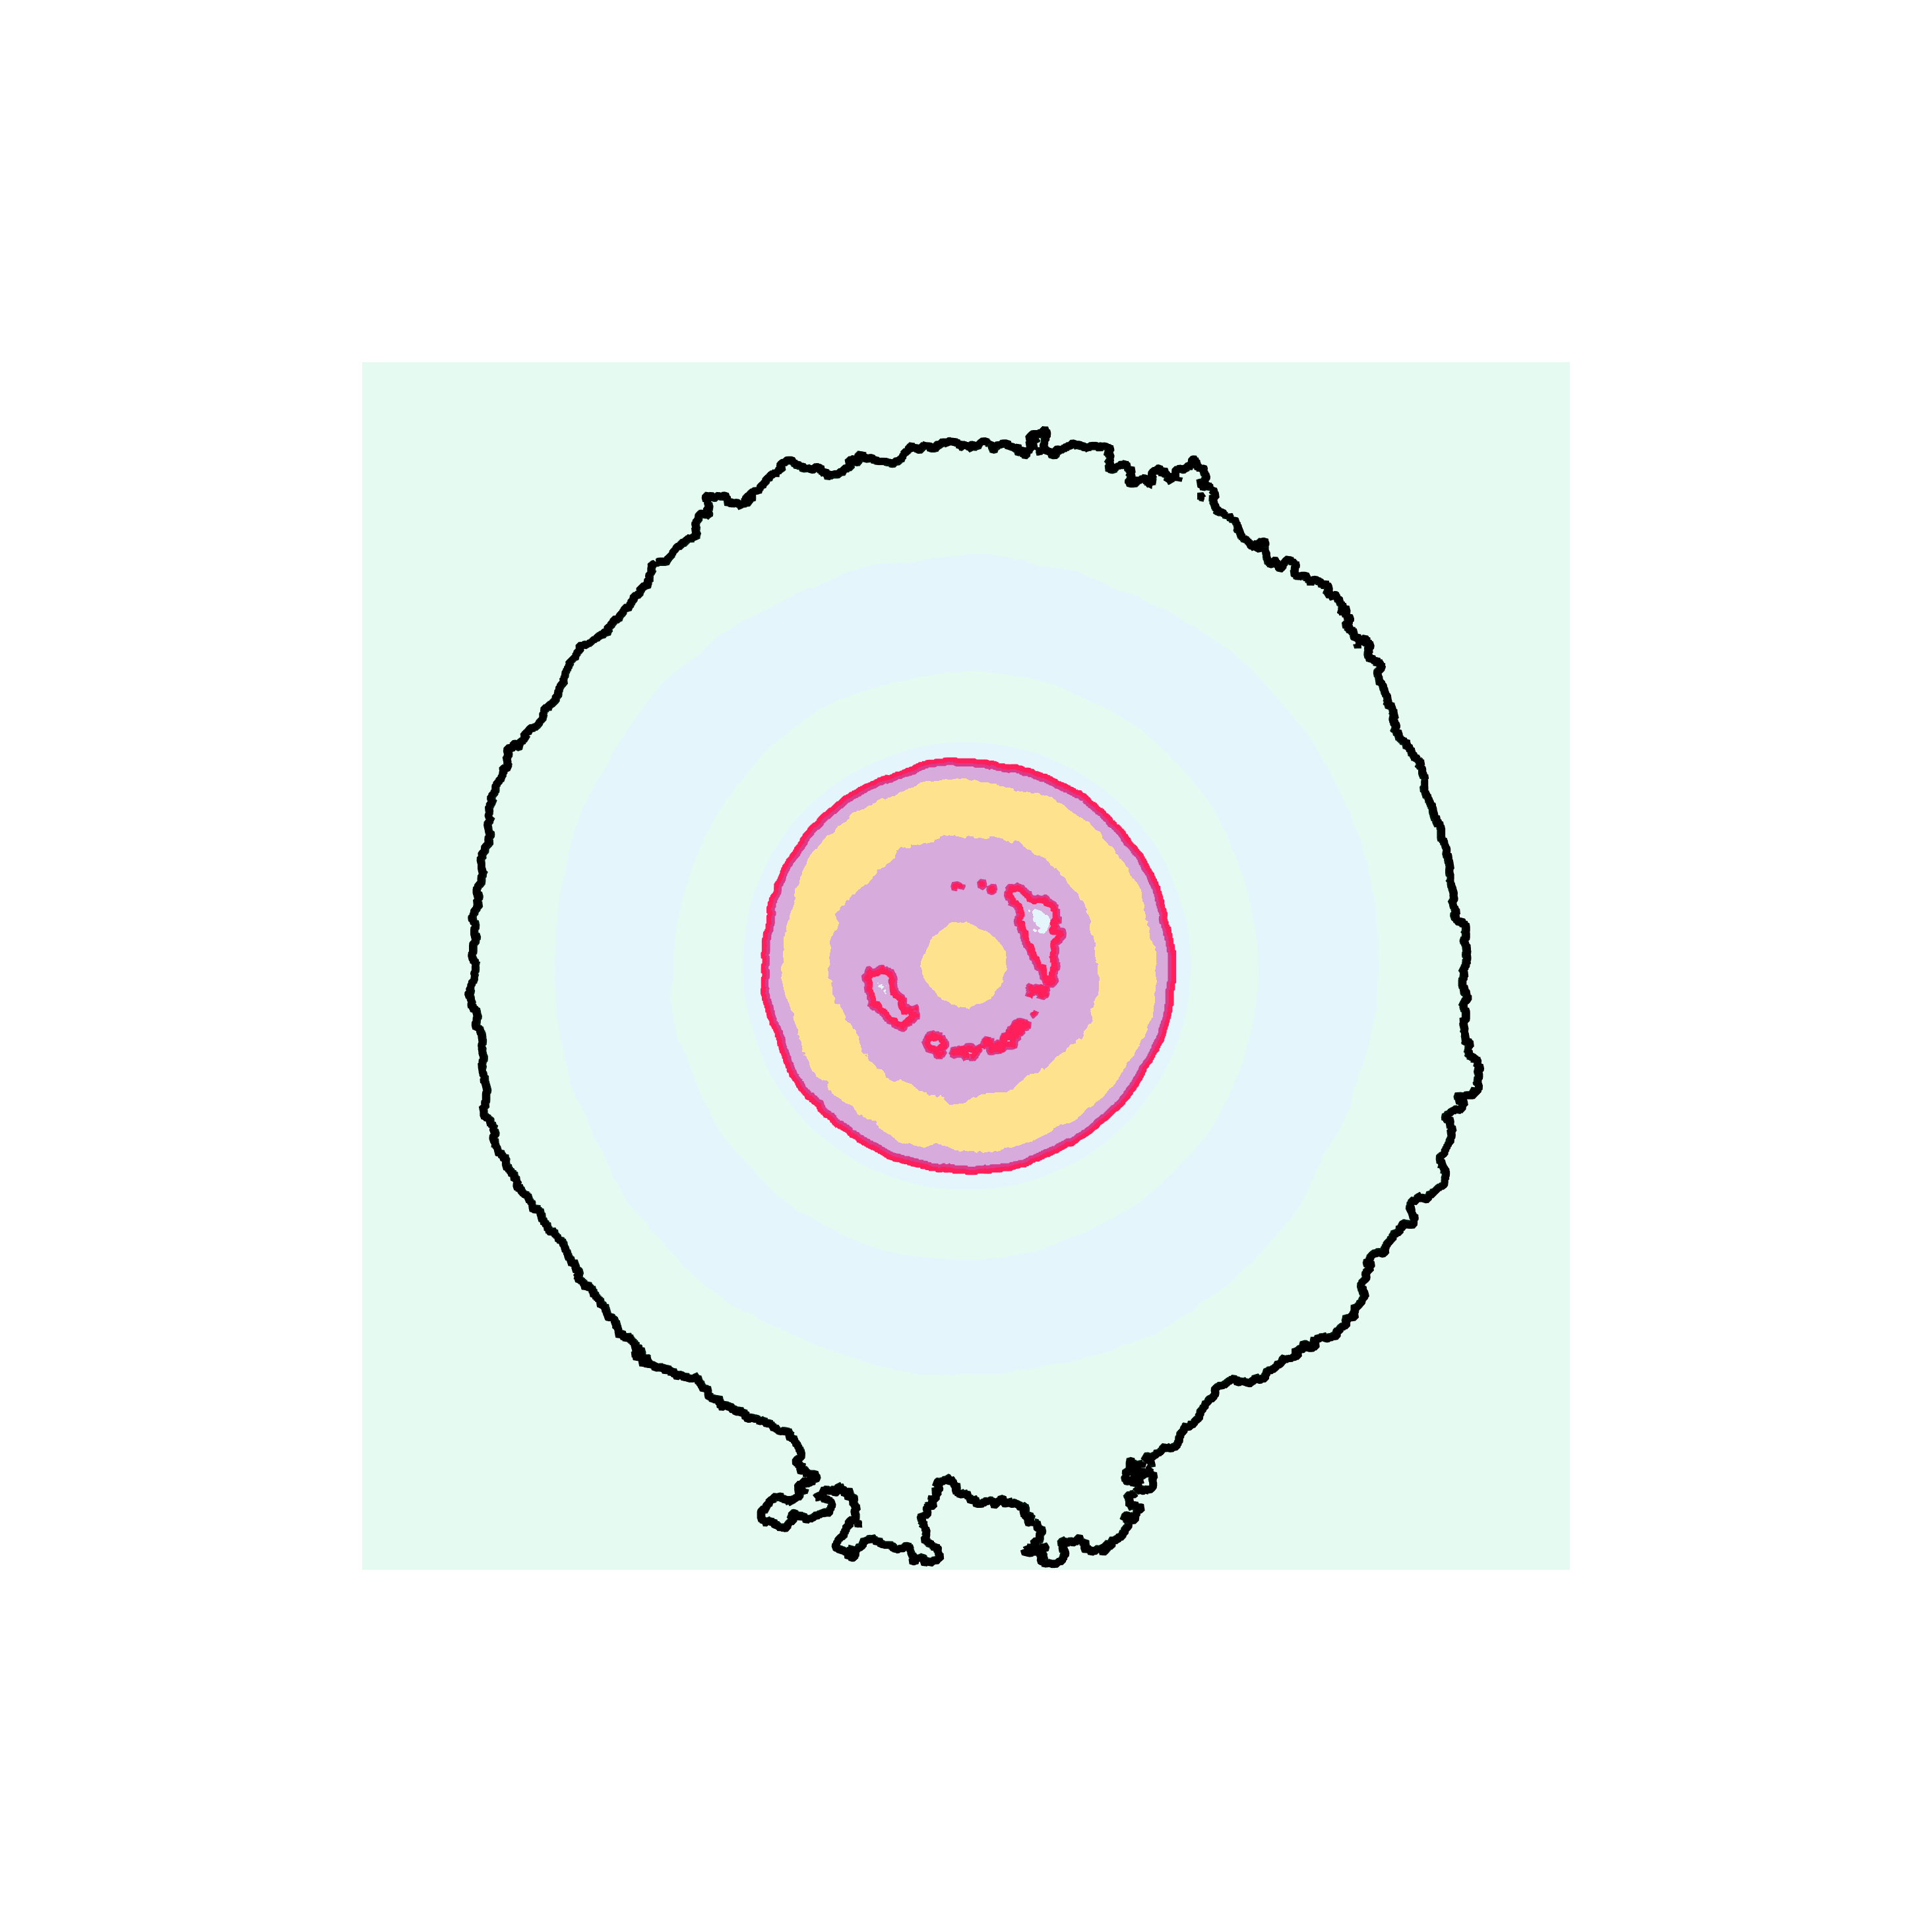
\includegraphics[trim=500 500 500 500, clip, width=0.24\textwidth]{scripts/figures/matching2/surf_top-1_1.png}
  
\includegraphics[trim=500 500 500 500, clip, width=0.24\textwidth]{scripts/figures/matching2/surf_top-1_2.png}
  \caption{(Top) $\hom_1$ persistence diagrams of the function depicted in Figure~\ref{fig:ripple1} restricted at $\omega = 0.3, 0.5,$ and $0.7$ (on a $1024\times 1024$ grid).
          The matching is shown between a feature in the full diagram (marked with a diamond) with its representative cycle in black.
          The corresponding representative cycle in the restricted diagram is pictured in red.}
\end{figure}
 % 96
% !TeX root = ../../main_socg.tex

In this section we will discuss a number of experiments which illustrate the benefit of truncated diagrams, and their approximation by relative diagrams, in comparison to their restricted counterparts.
We will focus on the persistent homology of functions on a square 2d grid.%---that is, functions with non-trivial persistent homology in dimensions zero and one.
% While these experiments can be conducted in dimension zero or one we will focus on $\hom_1$.
We chose as our function a radially symmetric damped sinusoid with random noise, depicted in Figure~\ref{fig:ripple1}, as it has prominent persistent homology in dimension one.

\paragraph*{Experimental setup.}

\begin{figure}[htbp]
  \centering
  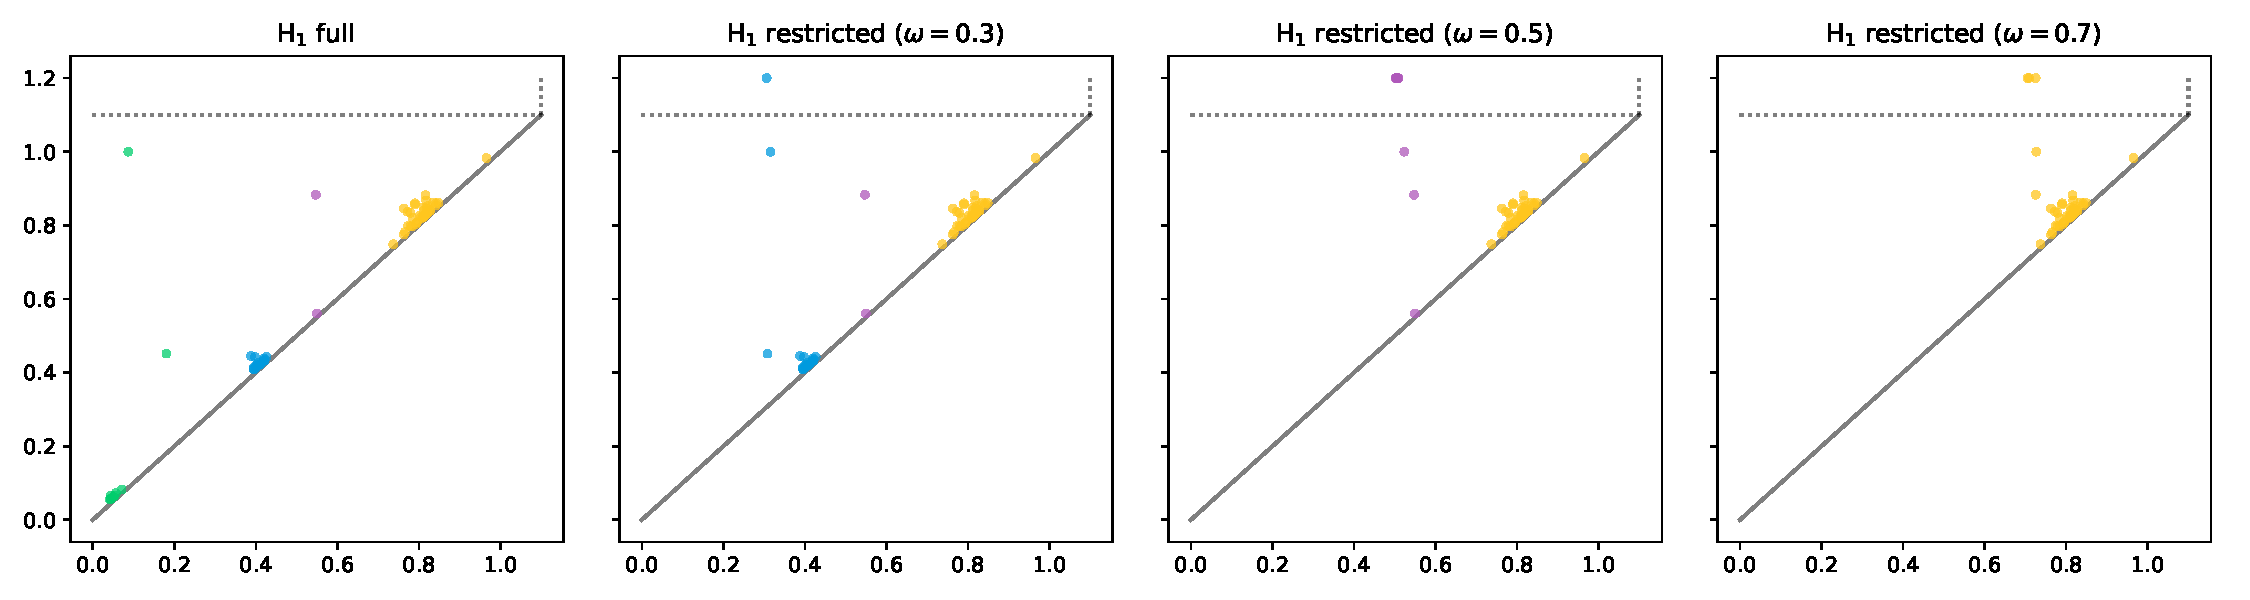
\includegraphics[trim=0 0 790 0, clip, width=0.3\textwidth]{scripts/figures/matching2/full-dgm.pdf}
  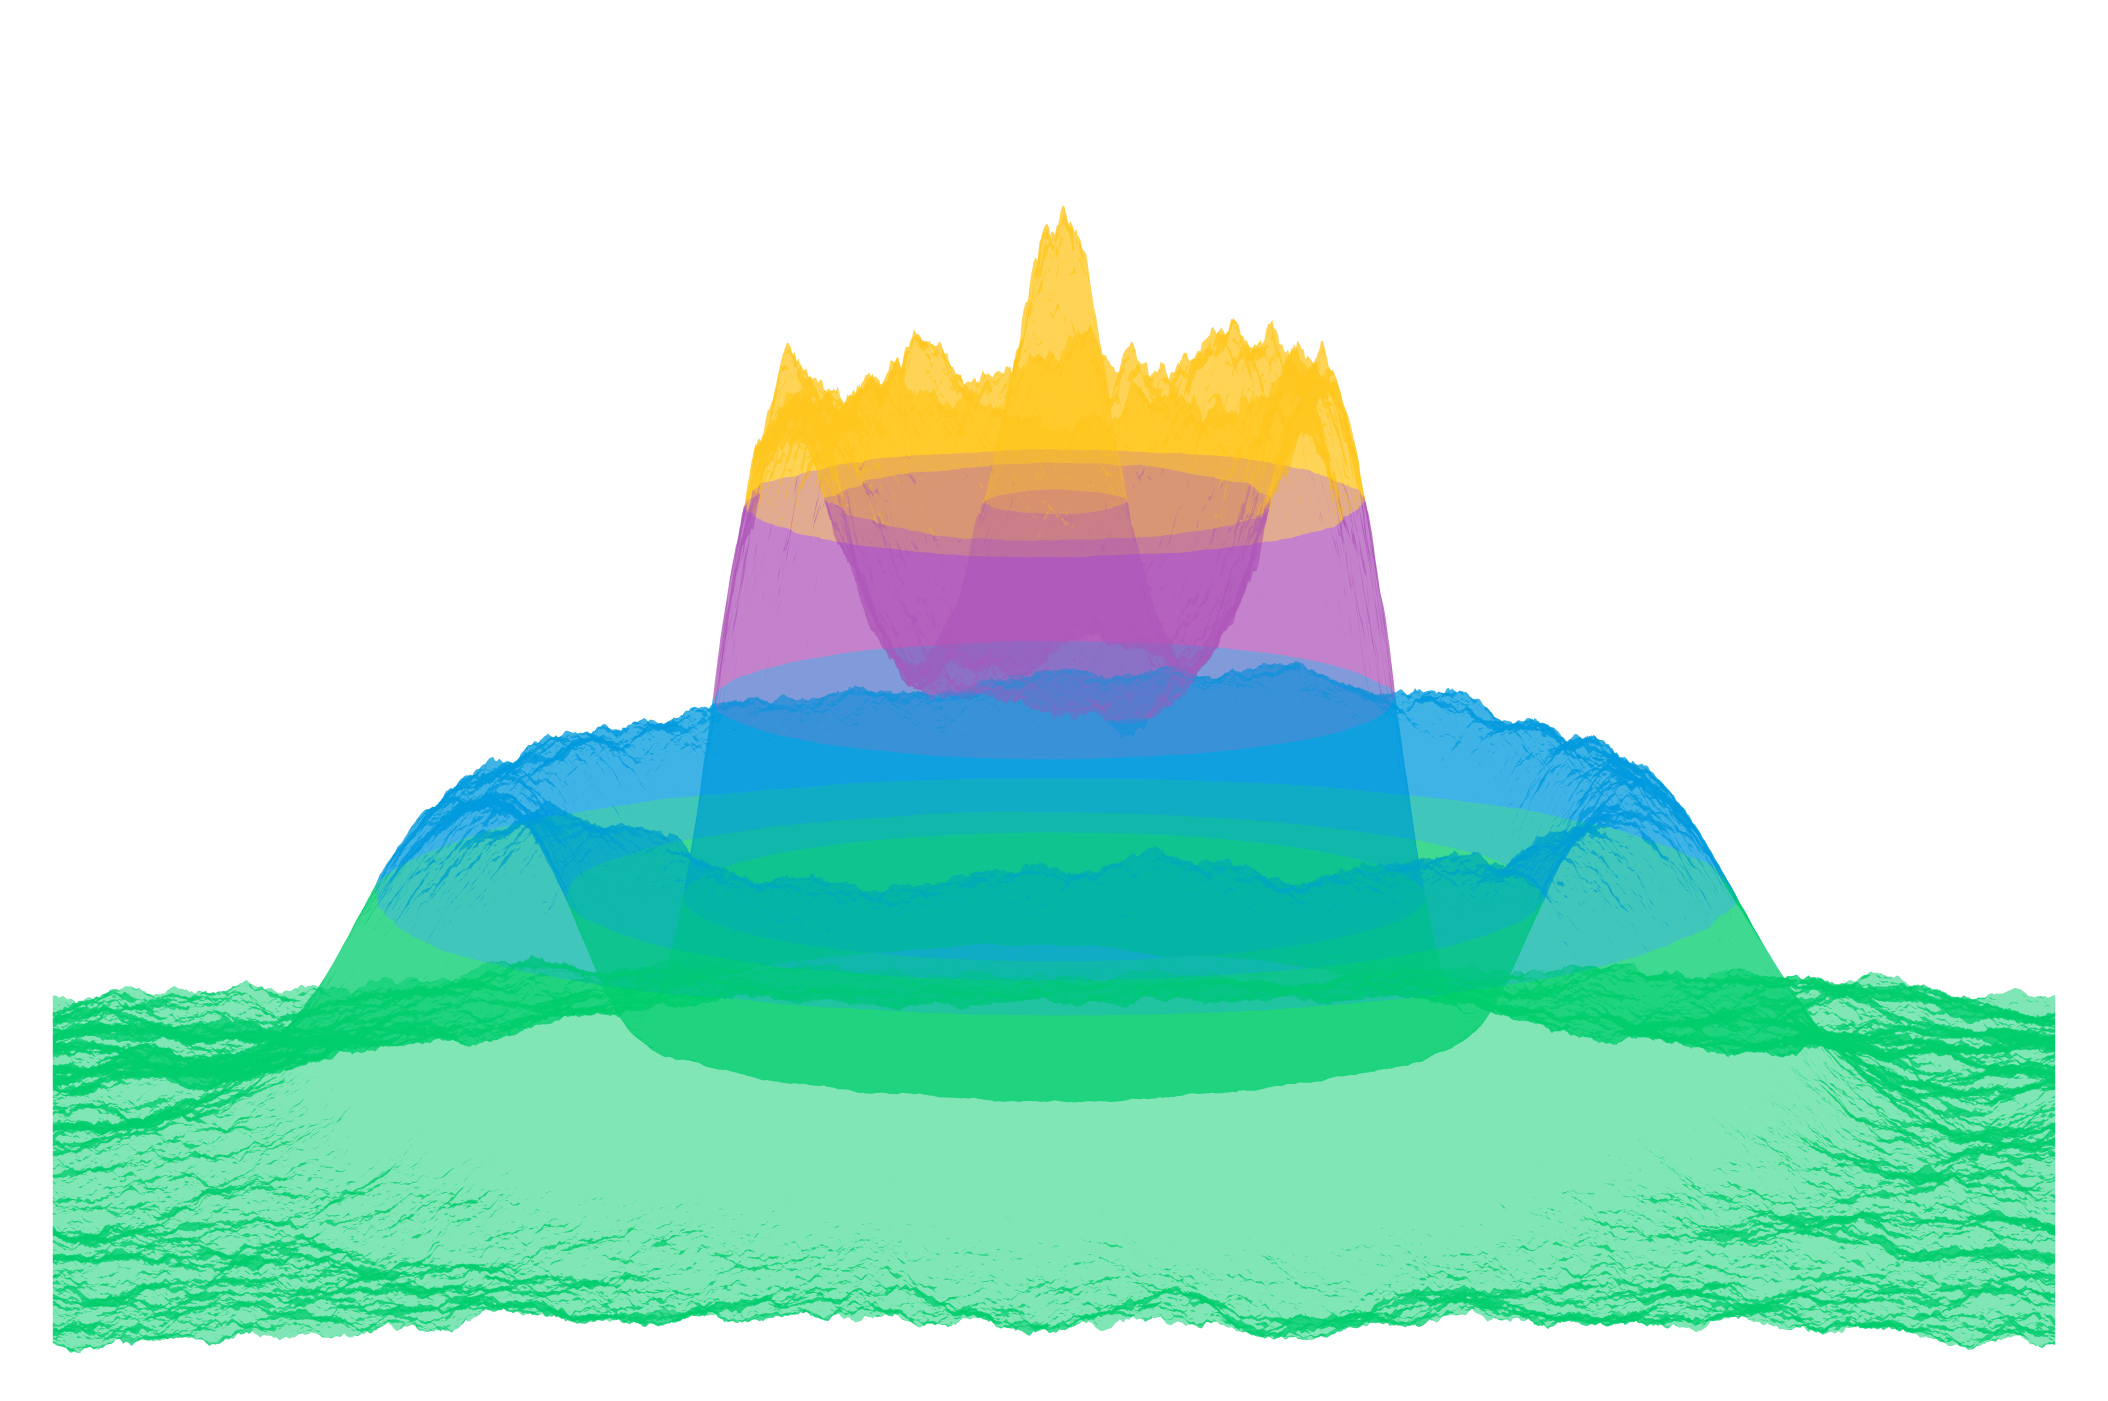
\includegraphics[trim=-350 -800 -700 -300, clip, width=0.4\textwidth]{scripts/figures/matching2/full-surf_side-lowres.png}
  
\includegraphics[trim=0 -800 0 0, width=0.25\textwidth]{scripts/figures/matching2/full-surf_top-lowres.png}
  % \includegraphics[trim=0 0 0 -10, clip, width=\textwidth]{scripts/figures/matching1/817_1024-3_1-1_1.png}
  \caption{The $\hom_1$ persistence diagram of the sinusoidal function pictured to the right.
  Features are colored by birth time, infinite features are drawn above the dotted line.}\label{fig:ripple1}
\end{figure}

Throughout, the four interlevel sets shown correspond to the ranges $[0, 0.3)$, $[0.3, 0.5)$, $[0.5, 0.7)$, and $[0.7, 1)$, respectively.
Our persistent homology computations were done primarily with Dionysus augmented with custom software for computing representative cycles of infinite features.
\footnote{3D figures were made with MayAvi, all other figures were made with Matplotlib.}
The persistent homology of our function was computed with the lower-star filtration of the Freudenthal triangulation on an $N\times N$ grid over $[-1,1]\times[-1,1]\subset\R^2$.
We take this filtration as $\{\rips^{2\delta}(P_\alpha)\}$ where $P$ is the set of grid points and $\delta = \sqrt{2} / N$.

We note that the purpose of these experiments is not to demonstrate the effectiveness of our approximation by Rips complexes, but to demonstrate the relationships between restricted, relative, and truncated diagrams.
Therefore, for simplicity, we will omit the inclusion $\rips^{2\delta}(P_\alpha)\hookrightarrow\rips^{4\delta}(P_\alpha)$ and take the persistent homology of $\{\rips^{2\delta}(P_\alpha)\}$ with sufficiently small $\delta$ as our ground-truth.
% However, in order to keep our diagrams clean we show only those features a distance at least $4\delta$ from the diagonal.
% Note that these features are \emph{not} removed from the diagram, and considered in all computations.

In the following we will take $N = 1024$, so $\delta\approx 1.4\times 10^{-3}$, as our ground-truth.
Figure~\ref{fig:ripple1} shows the \emph{full diagram} of our function with features colored by birth time.
Therefore, for $\omega = 0.3, 0.5, 0.7$ the \emph{truncated diagram} is obtained by successively removing features in each interlevel set.
Recall the \emph{restricted diagram} is that of the function restricted to the $\omega$ \emph{super}-levelset filtration, and computed with $\{\rips^{2\delta}(P_\alpha\setminus Q_\omega)\}$.
We will compare this restricted diagram with the \emph{relative diagram}, computed as the relative persistent homology of the filtration of pairs $\{\rips^{2\delta}(P_\alpha, Q_\omega)\}$.

\paragraph*{The issue with restricted diagrams.}

% In order to get an initial sense of the difference between relative and restricted diagrams we first compare the bottleneck distance of each to the truncated diagram.
% As we have shown the relative diagram is equal to the truncated diagram with additional infinite features we will remove all infinite features from the bottleneck computation.
% We therefore expect the distance between the relative and truncated diagrams to be zero for $N=1024$.

Figure~\ref{fig:bottleneck} shows the bottleneck distance from the truncated diagram at full resolution ($N = 1024$) to both the relative and restricted diagrams with varying resolution.
Specifically, the function on a $1024\times 1024$ grid is down-sampled to grids ranging from $64\times 64$ to $1024\times 1024$.
We also show the expected bottleneck distance to the true truncated diagram given by the interleaving in Theorem~\ref{thm:interleaving_main_2} in black.

\begin{figure}[htbp]\label{fig:bottleneck}
  \centering
  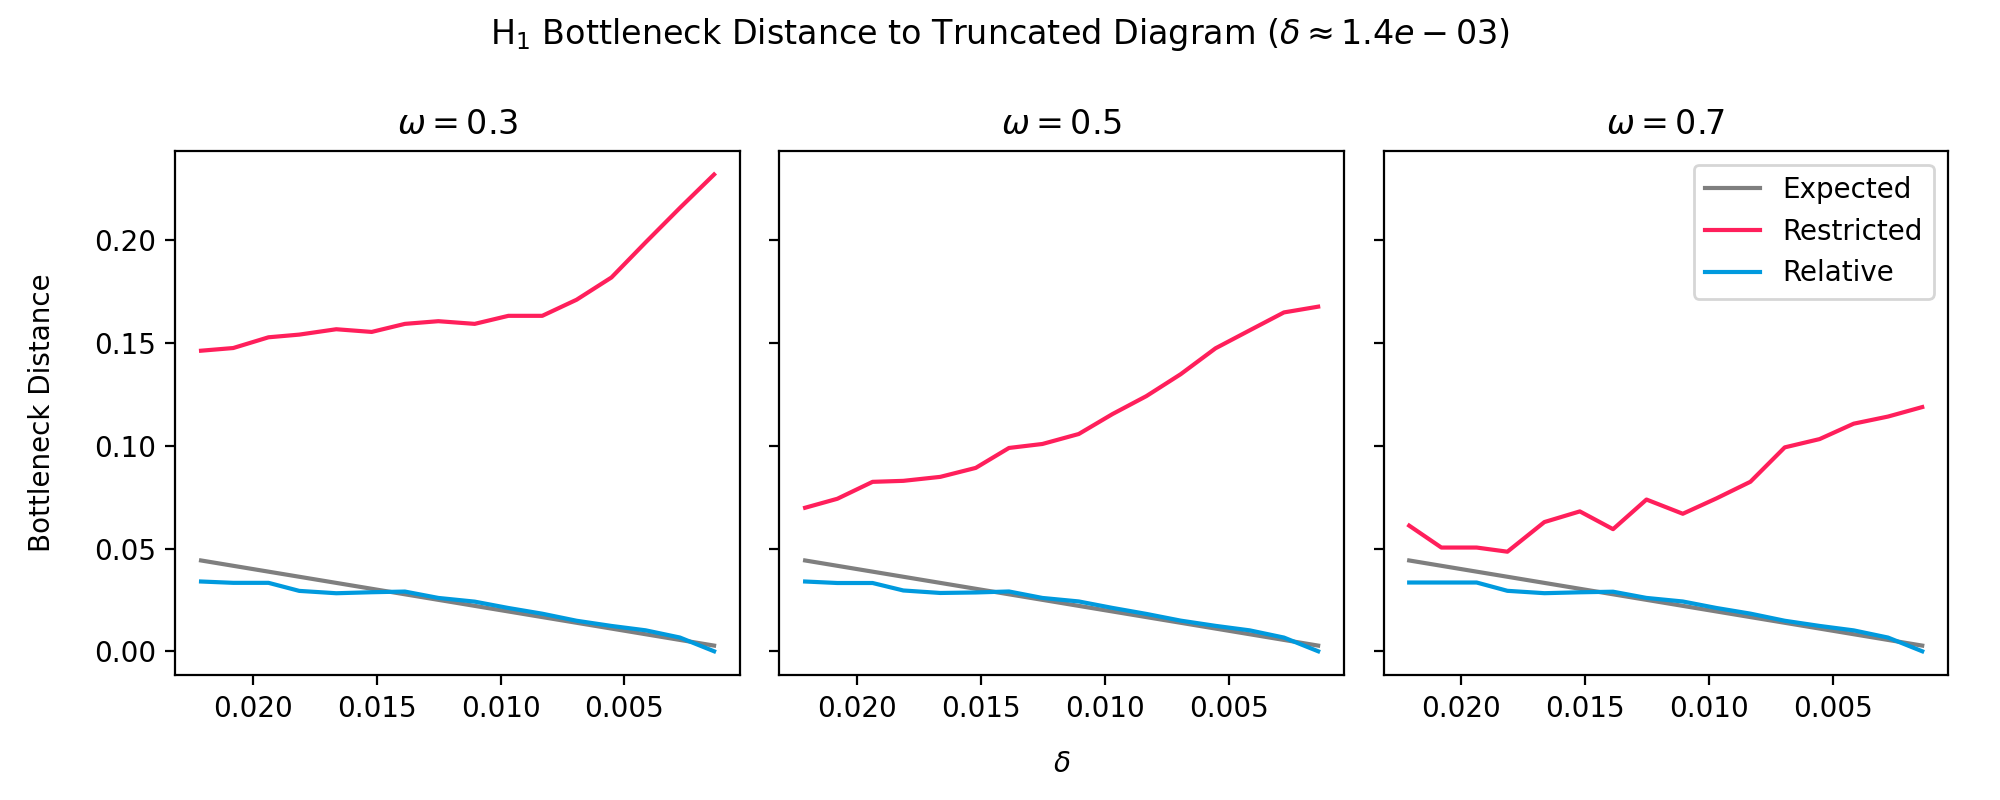
\includegraphics[width=\textwidth]{scripts/figures/matching2/bottleneck_delta.png}
  \caption{Comparison of the bottleneck distance between the truncated diagram and those of the restricted and relative diagrams with increasing resolution.}
\end{figure}

As we can see, the relative diagram clearly performs better than the restricted diagram, which diverges with increasing resolution.
% The reason for this is shown in Figure~\ref{fig:restricted} which depicts the restricted diagrams at $\omega = 0.3, 0.5,$ and $0.7$ at full resolution.
Recall that 1-dimensional features that are born before $\omega$ and die after $\omega$ become infinite 2-dimensional features in the relative diagram, with birth time equal to the death time of the corresponding feature in the full diagram.
These same features remain 1-dimensional figures in the restricted diagram, but with their birth times shifted to $\omega$.
% Indeed, the resulting restricted diagram may be closer to the full diagram for sufficiently small $\omega$.
% However, the distance will be proportional to the difference between $\omega$ and the true birth time.

\begin{figure}[htbp]
  \centering
  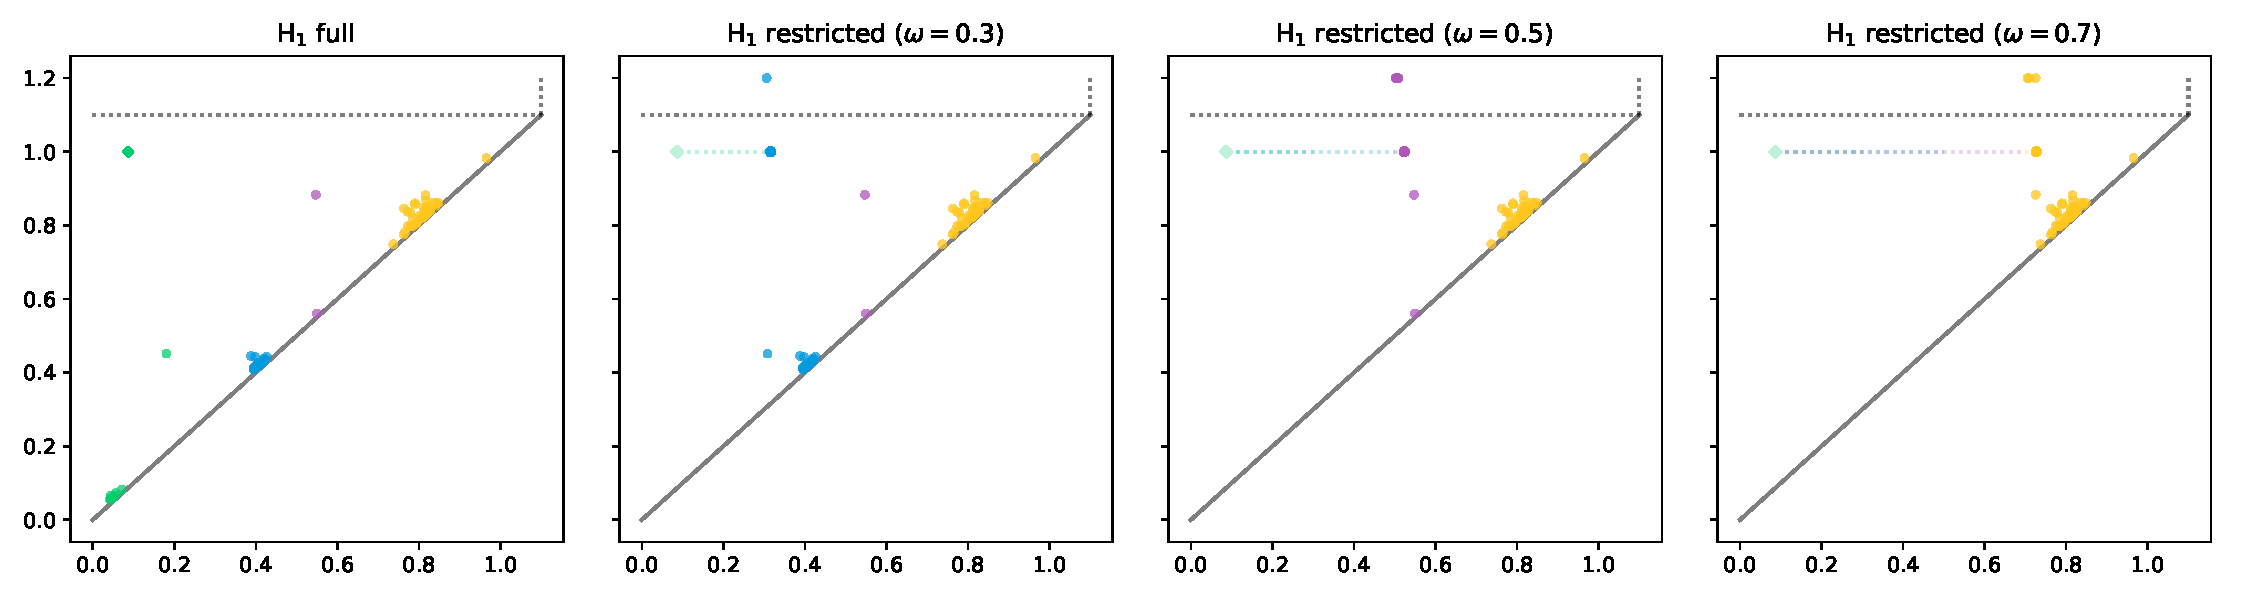
\includegraphics[trim=0 0 -10 0, clip, width=\textwidth]{scripts/figures/matching2/dgm-1.pdf}
  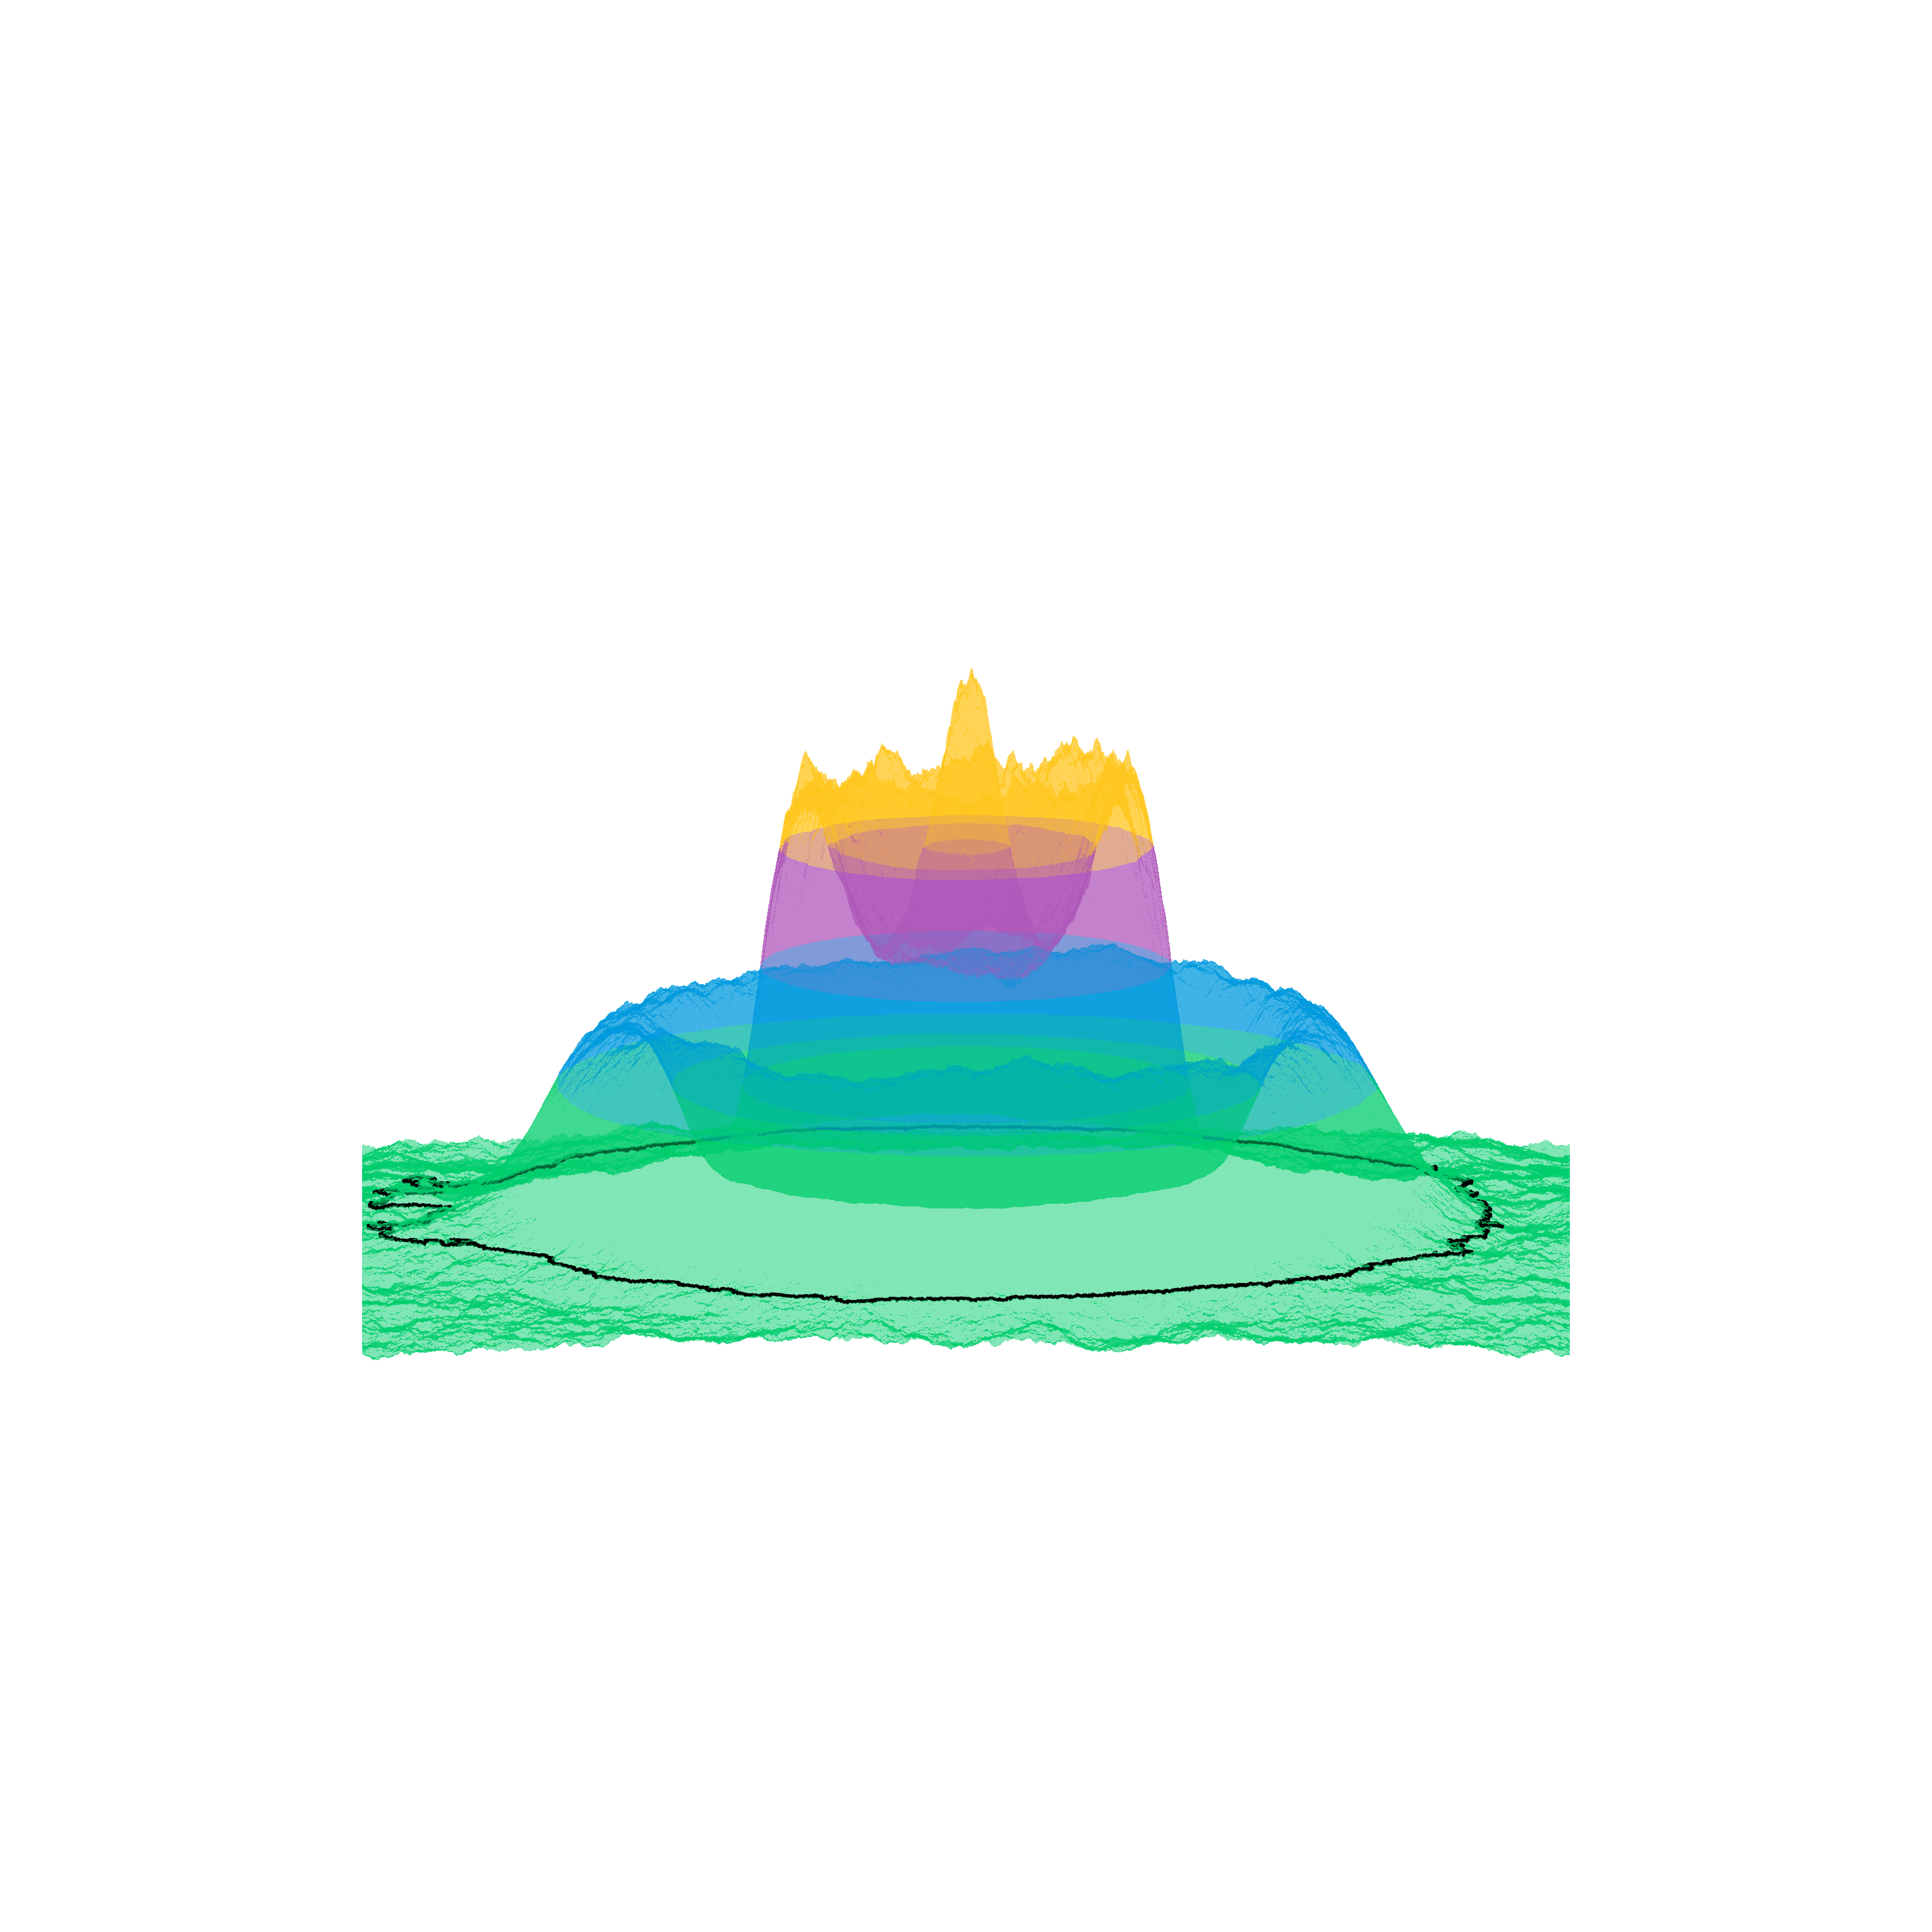
\includegraphics[trim=500 800 500 800, clip, width=0.24\textwidth]{scripts/figures/matching2/surf_side-1.png}
  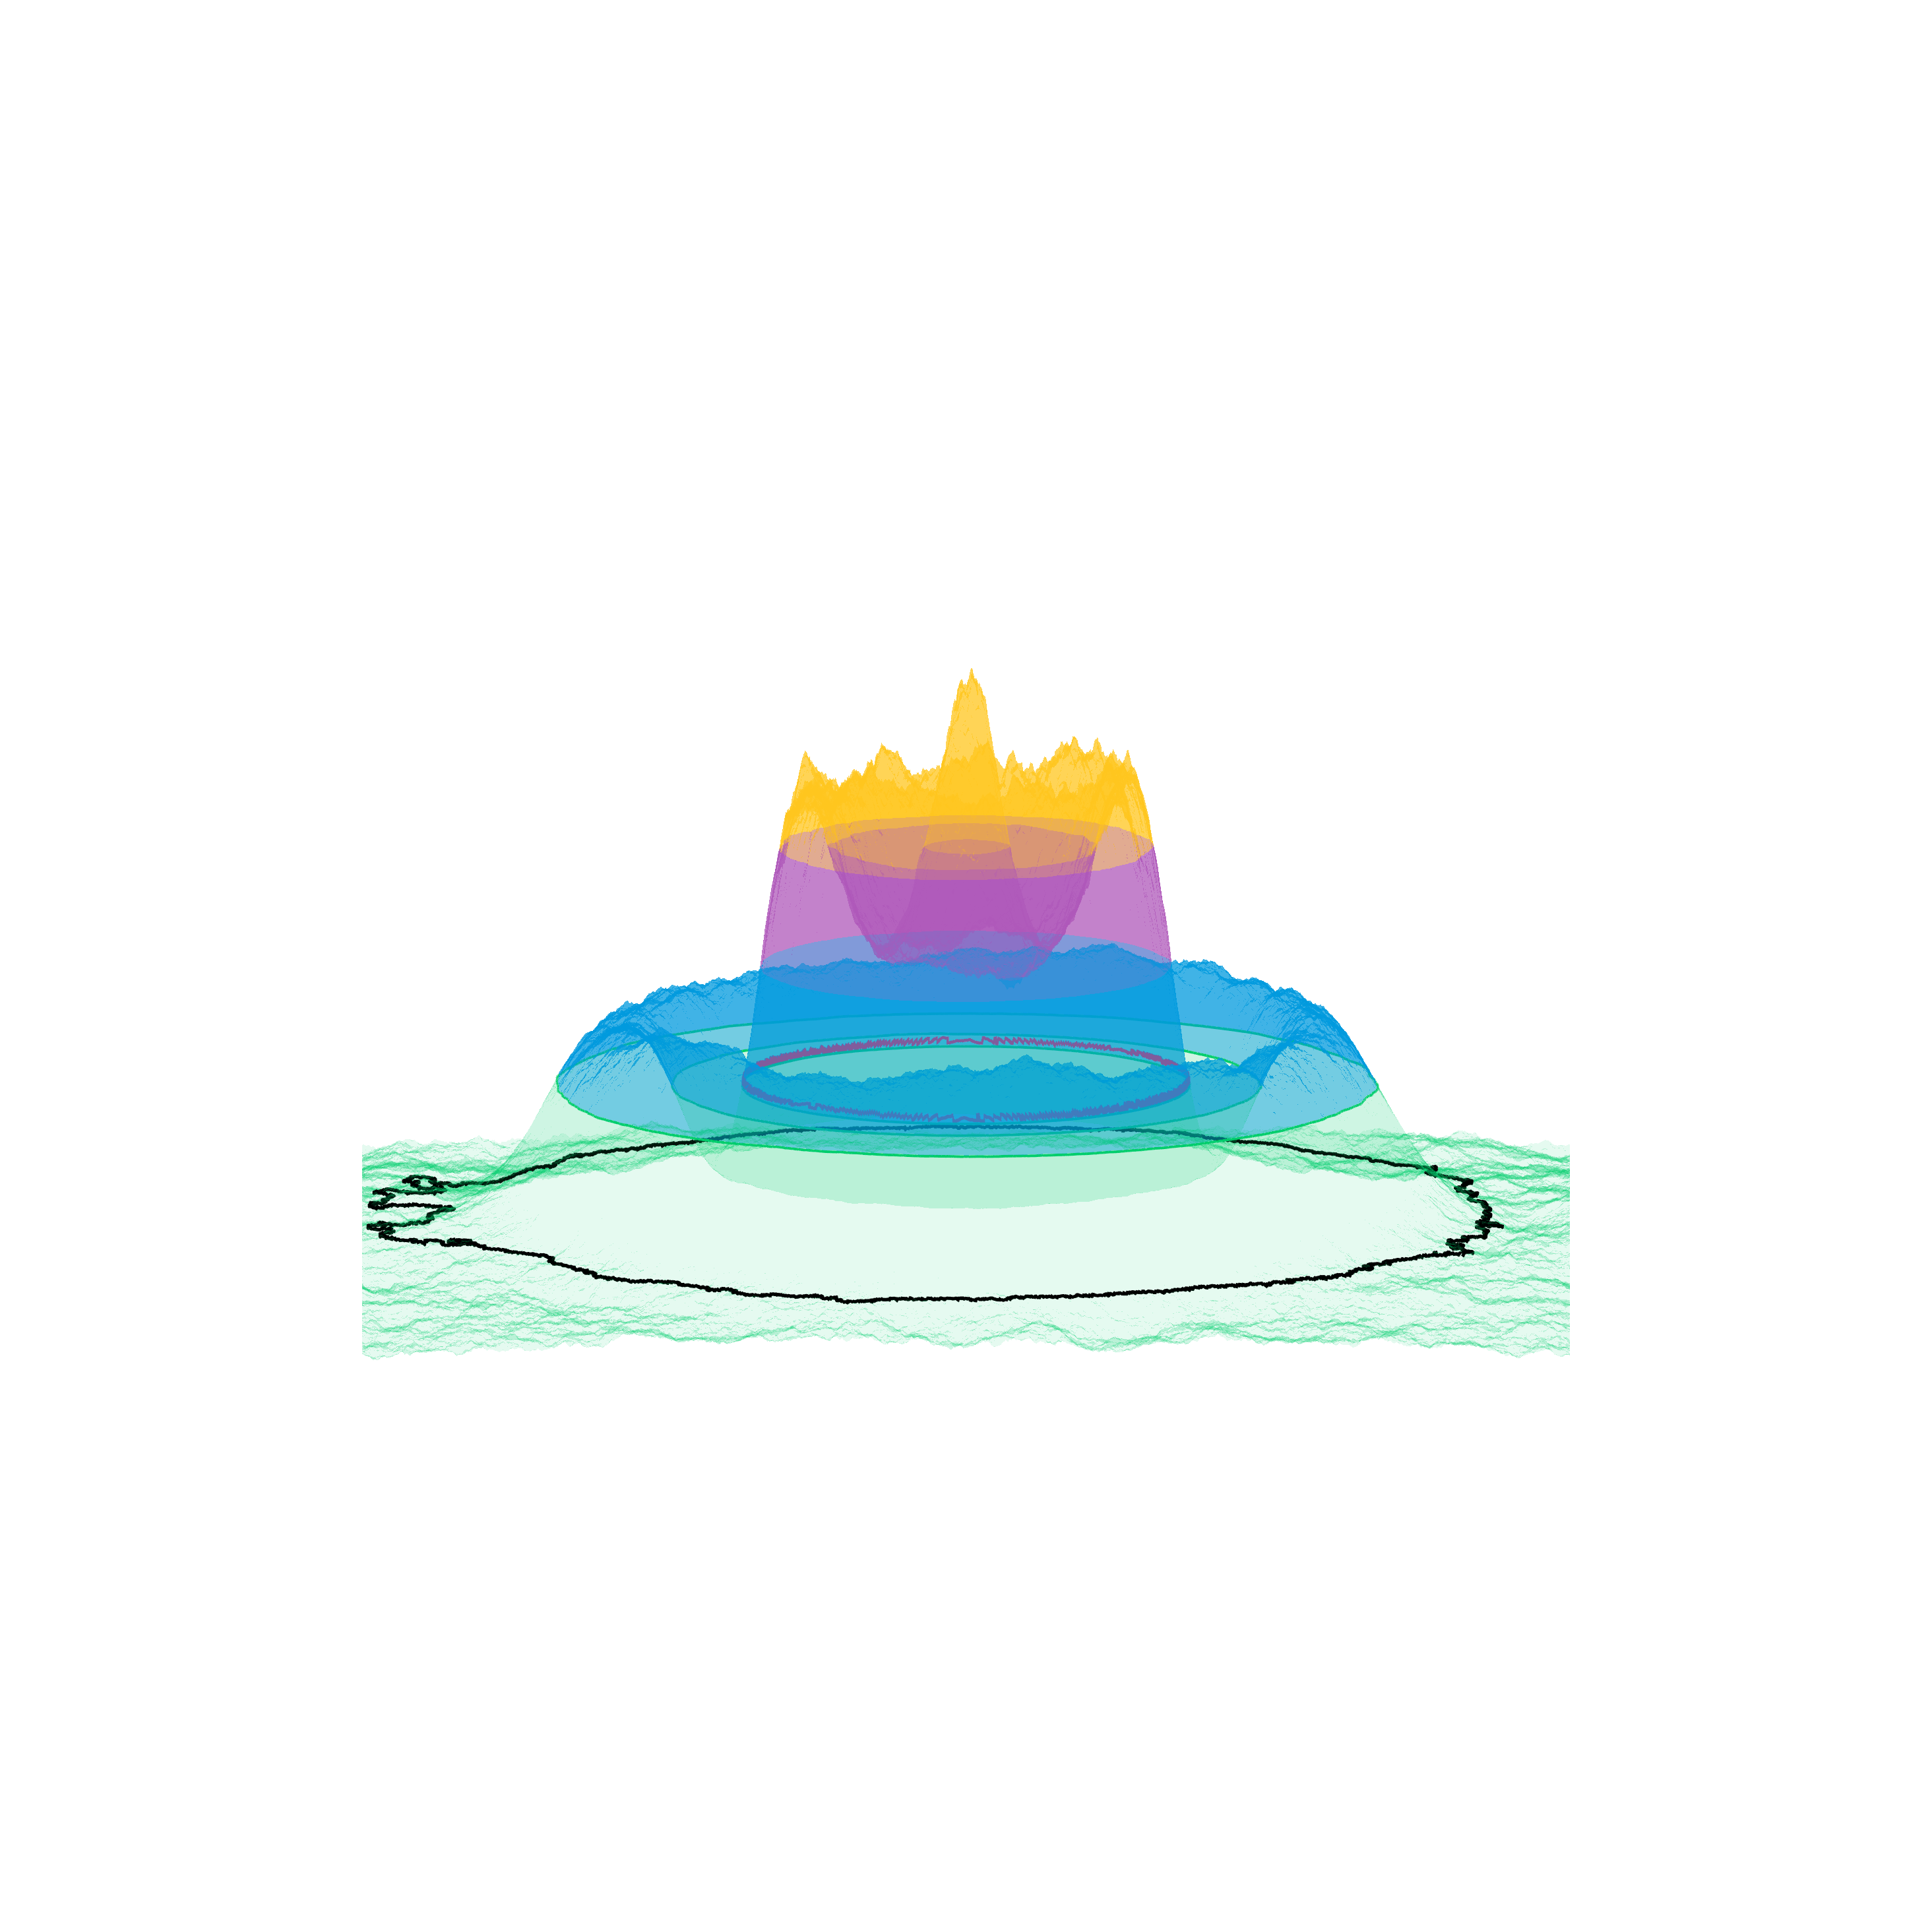
\includegraphics[trim=500 800 500 800, clip, width=0.24\textwidth]{scripts/figures/matching2/surf_side-1_0.png}
  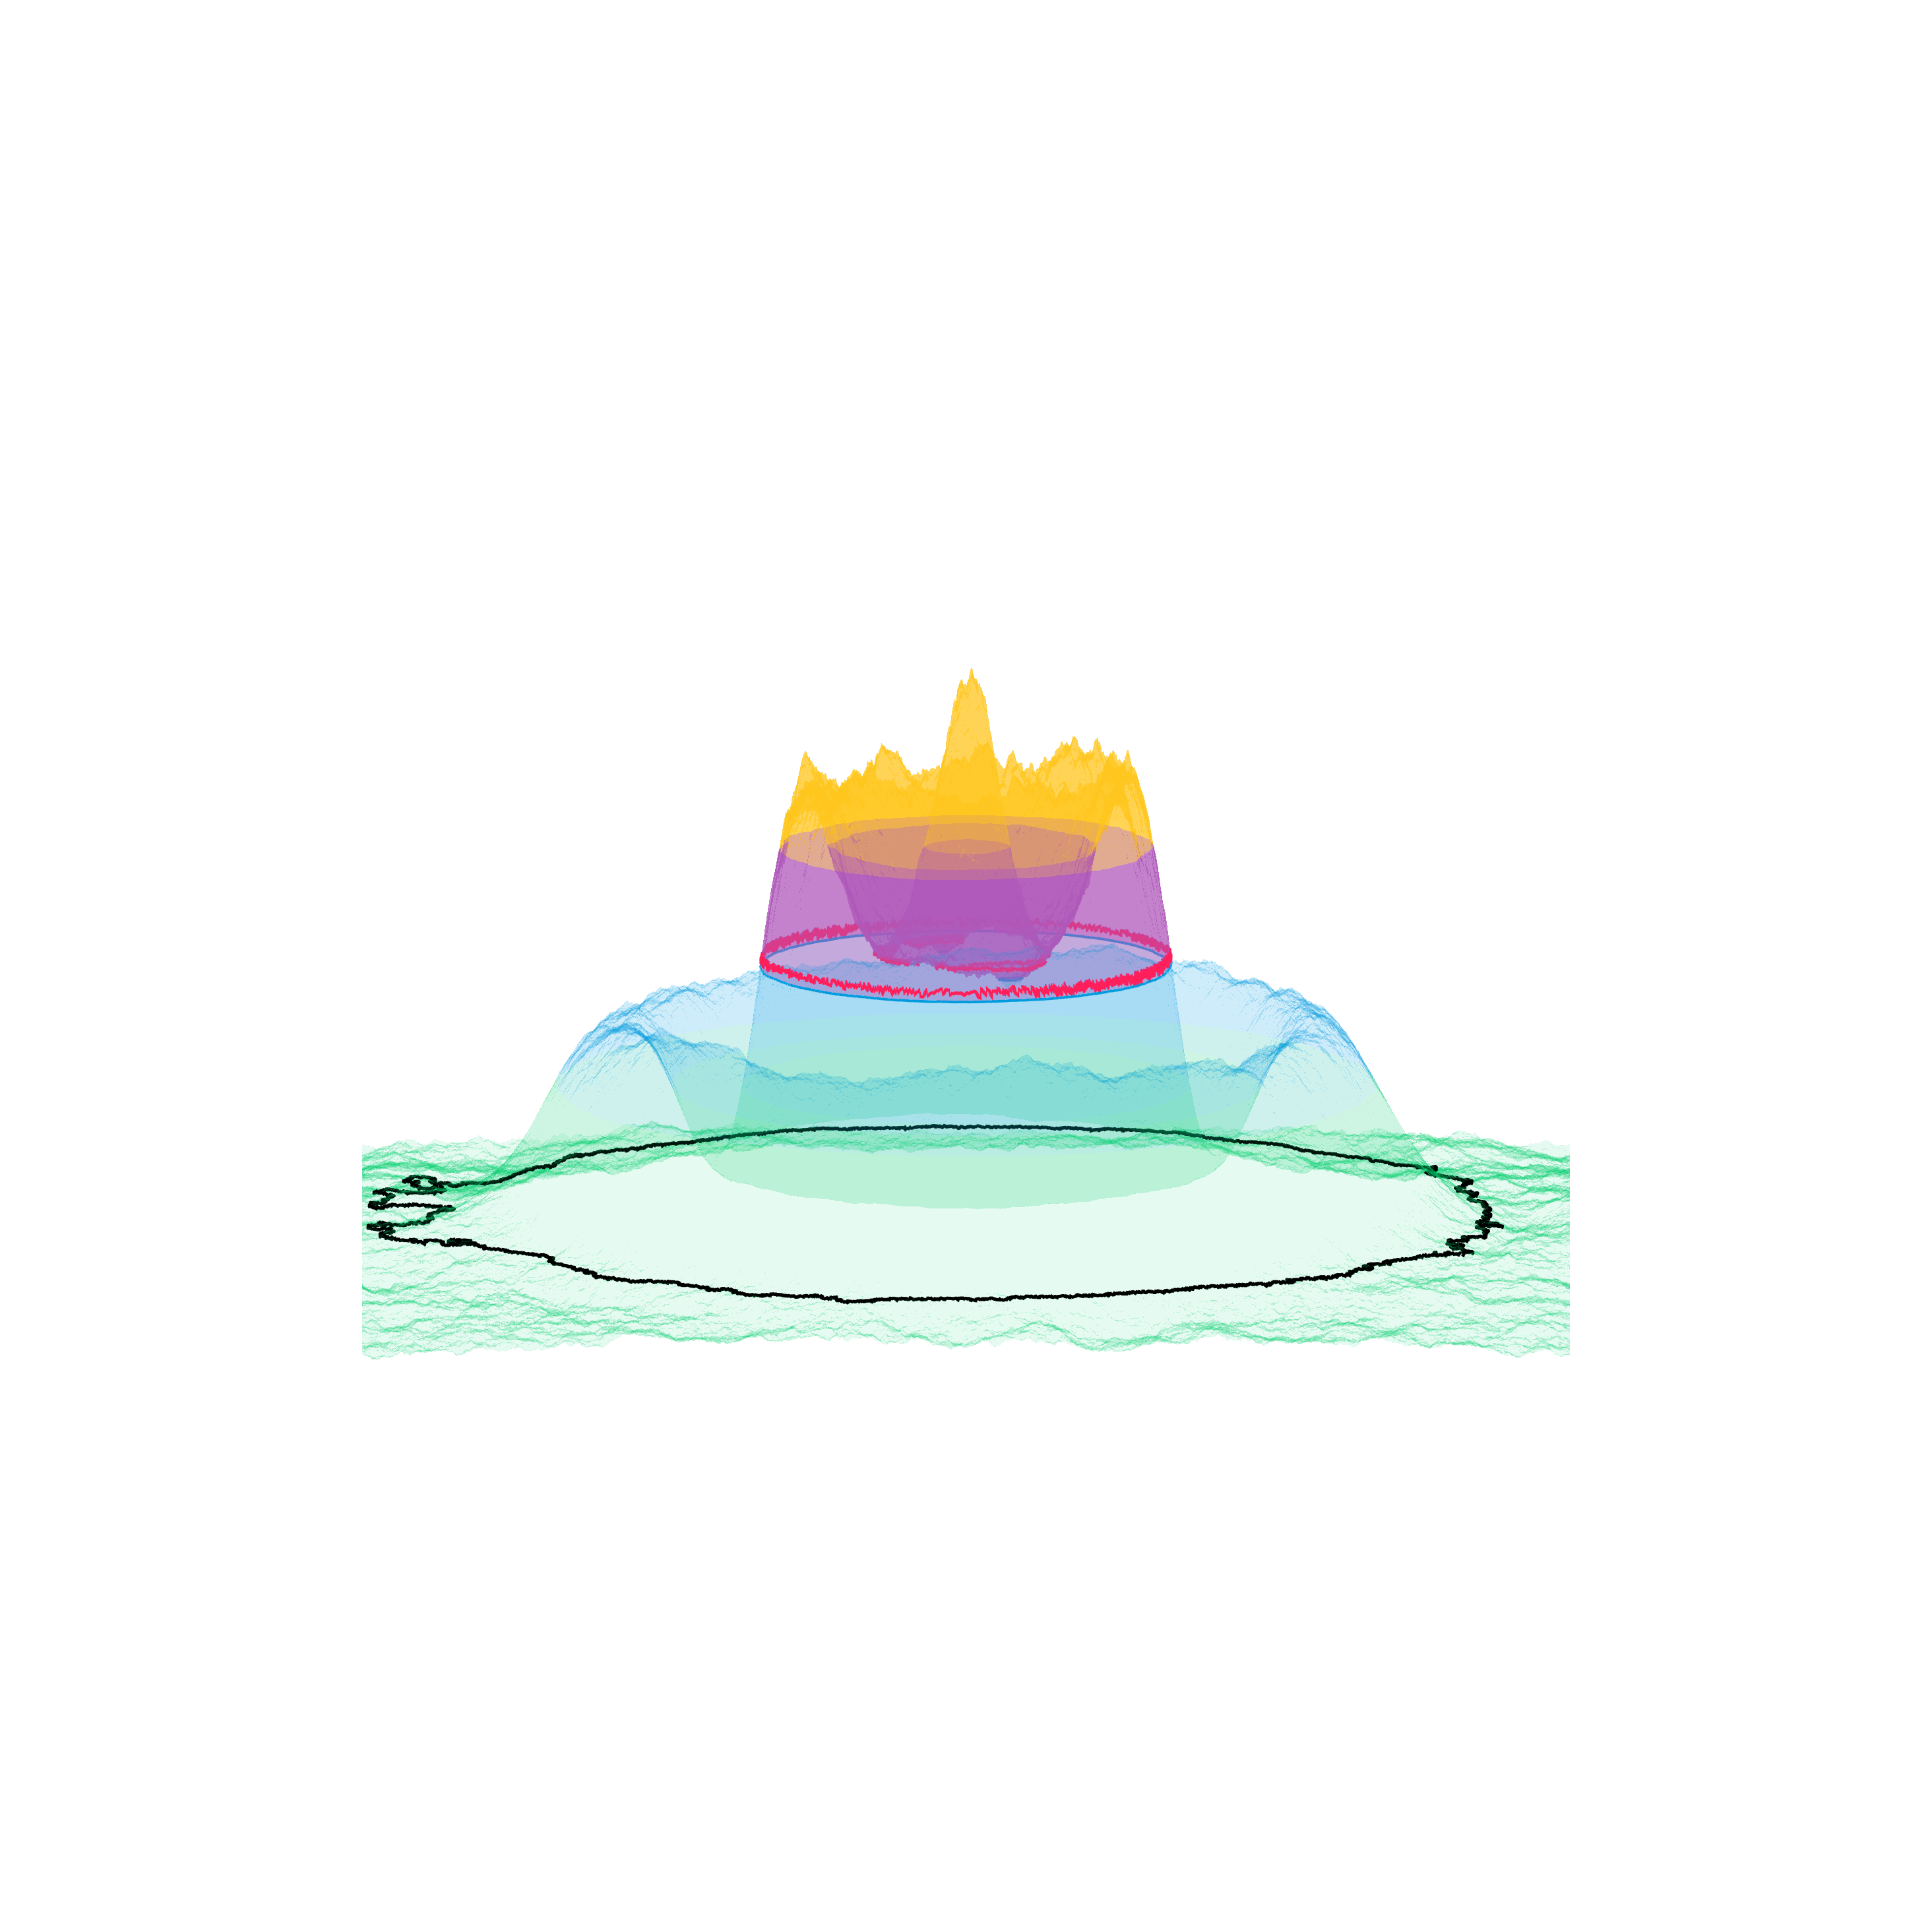
\includegraphics[trim=500 800 500 800, clip, width=0.24\textwidth]{scripts/figures/matching2/surf_side-1_1.png}
  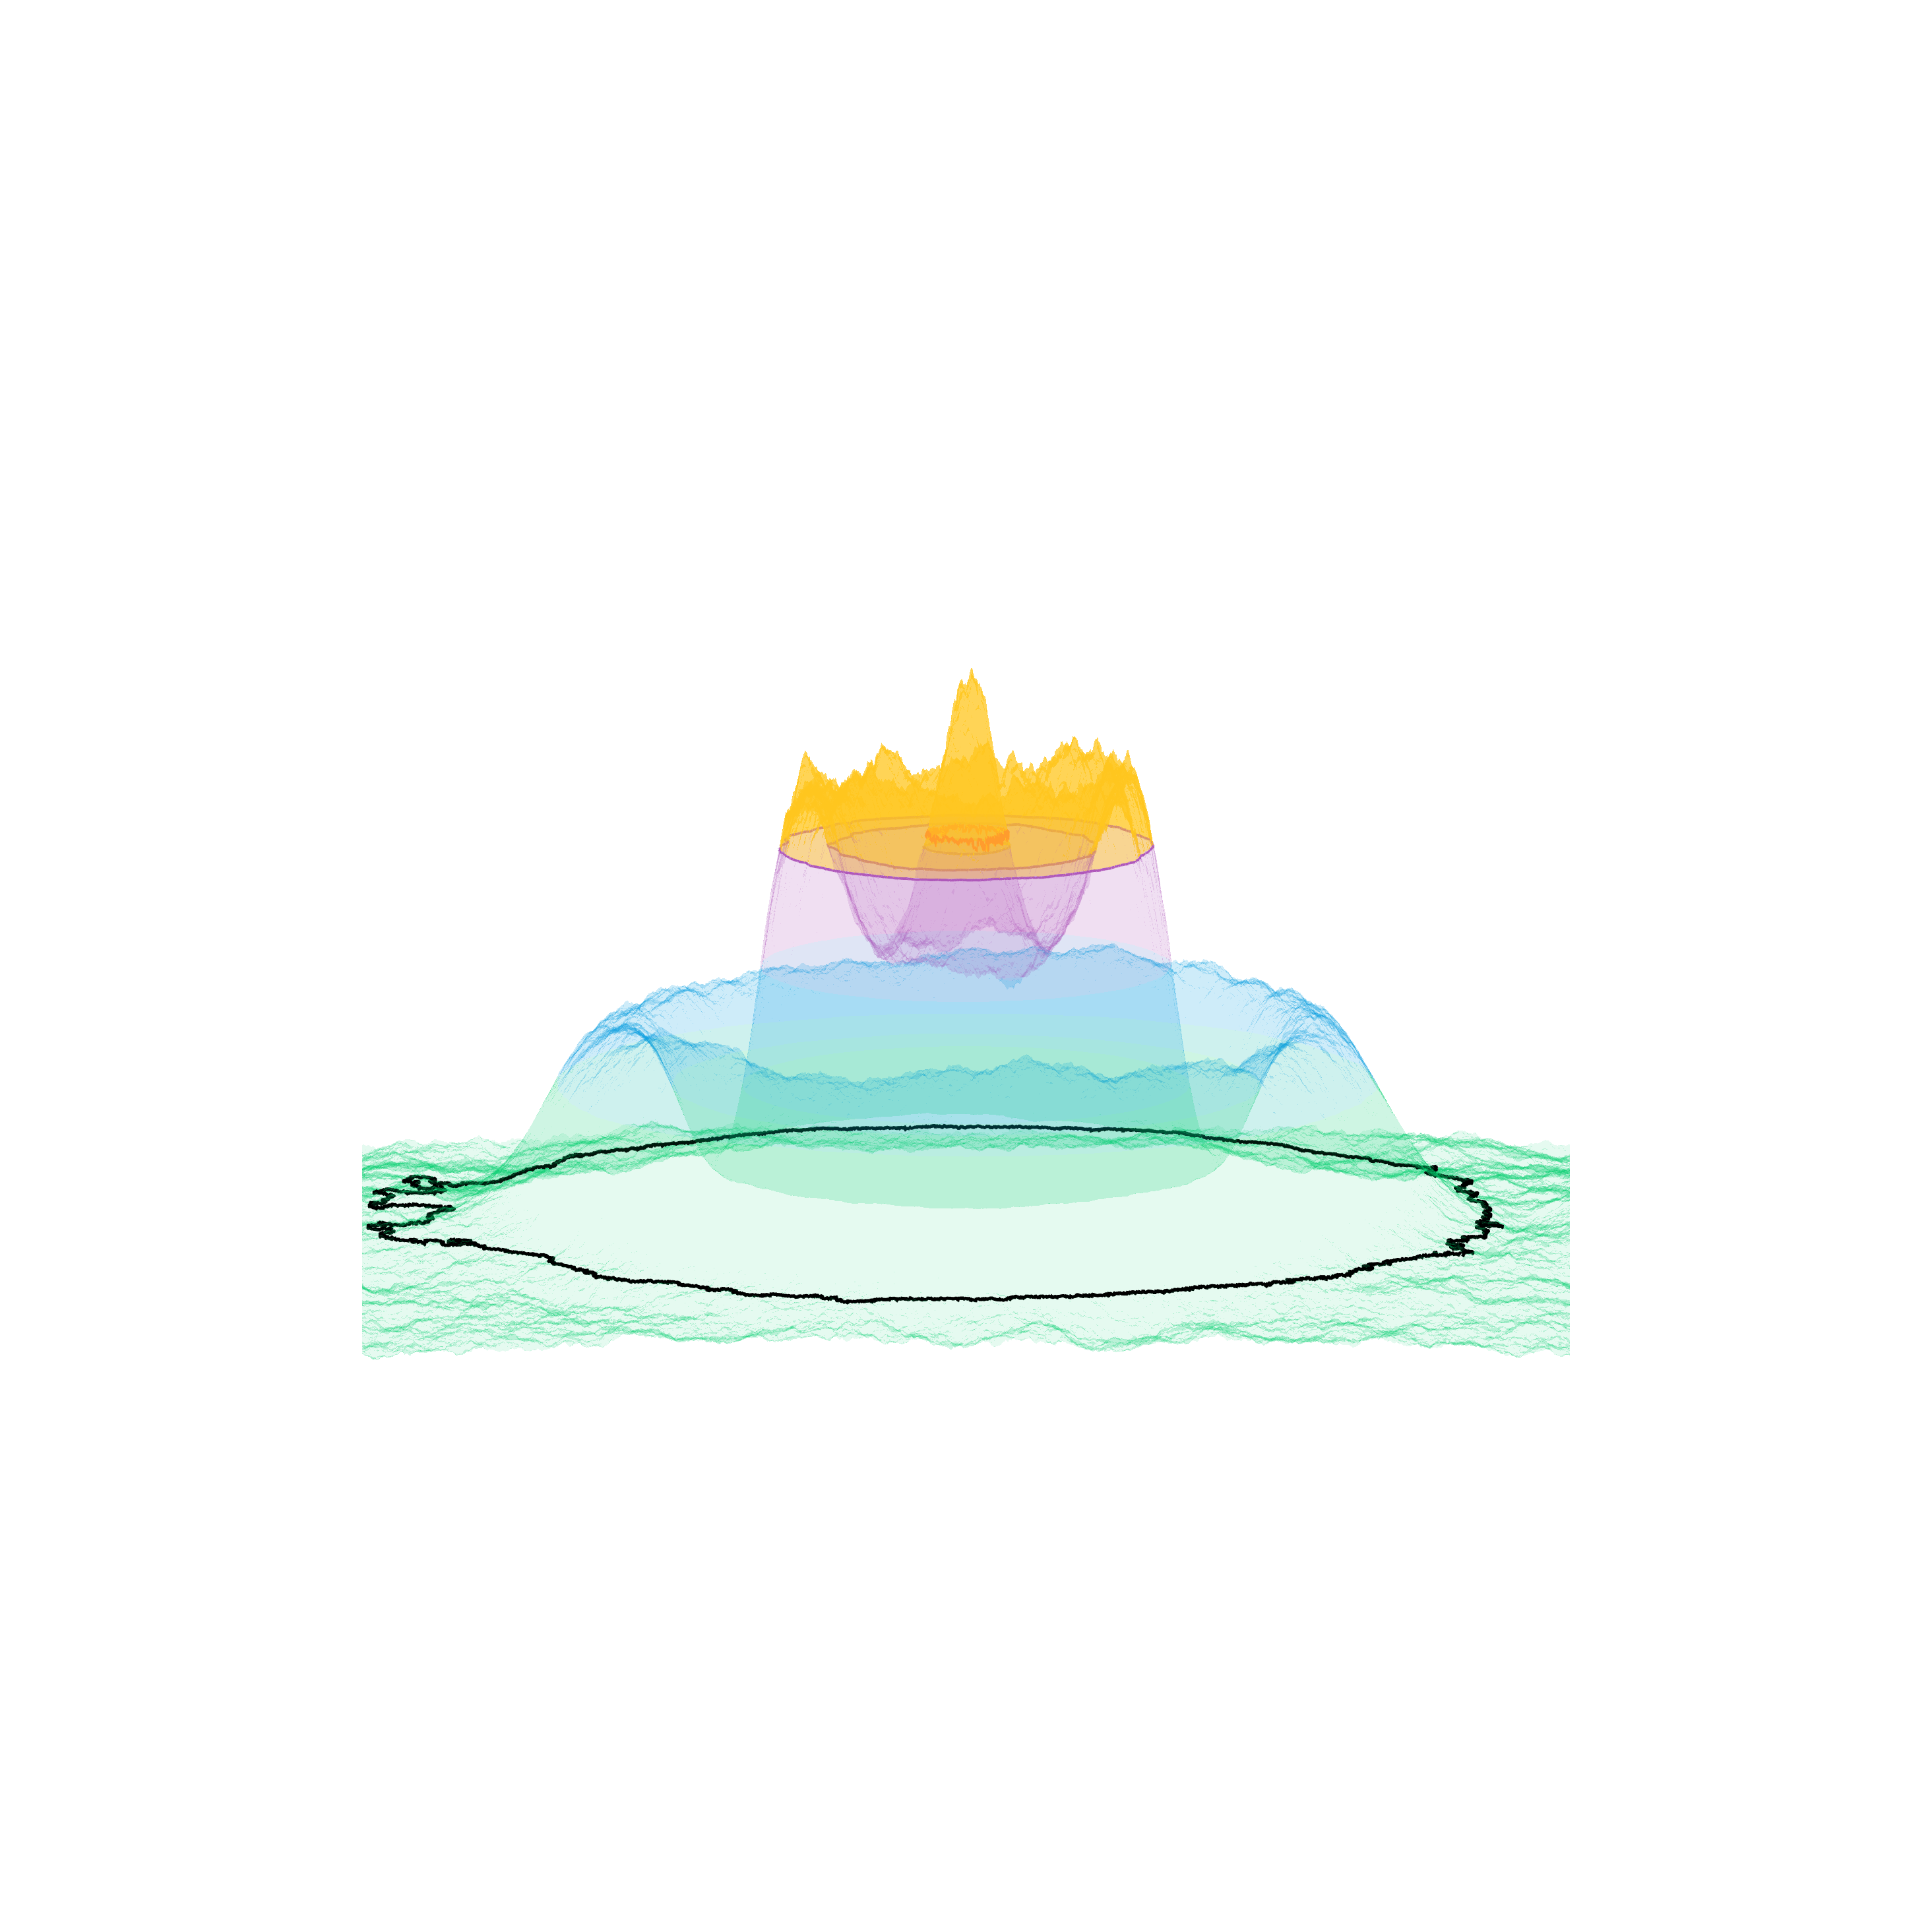
\includegraphics[trim=500 800 500 800, clip, width=0.24\textwidth]{scripts/figures/matching2/surf_side-1_2.png}
  \includegraphics[trim=500 500 500 500, clip, width=0.24\textwidth]{scripts/figures/matching2/surf_top-1.png}
  \includegraphics[trim=500 500 500 500, clip, width=0.24\textwidth]{scripts/figures/matching2/surf_top-1_0.png}
  \includegraphics[trim=500 500 500 500, clip, width=0.24\textwidth]{scripts/figures/matching2/surf_top-1_1.png}
  \includegraphics[trim=500 500 500 500, clip, width=0.24\textwidth]{scripts/figures/matching2/surf_top-1_2.png}
  \caption{(Top) $\hom_1$ persistence diagrams of the function depicted in Figure~\ref{fig:ripple1} restricted to \emph{super}-levelsets at $\omega = 0.3, 0.5,$ and $0.7$ (on a $1024\times 1024$ grid).
  The matching is shown between a feature in the full diagram (marked with a diamond) with its representative cycle in black.
  The corresponding representative cycle in the restricted diagram is pictured in red.}\label{fig:restricted}
\end{figure}

Figure~\ref{fig:restricted} shows this distance for a feature that persists throughout the diagram.
As the restricted diagram in full resolution the restricted filtration is a subset of the full filtration, so these features can be matched by their death simplices.
For illustrative purposes we also show the representative cycles associated with these features.

% We imagine a setting where we would like to classify a function using a sample that cannot be verified below some known $\omega$.
% That is, we can only check for coverage of the super-levelset $D\setminus B_\omega$ using the variation of the TCC we have introduced in the previous sections.
% We would then like to classify the function with the bottleneck distance to a set of known functions based on the region we cover.
% However, as we have shown, the restricted diagram may contain artifacts of features born before $\omega$ which will skew our measurement.
% Instead, as $\omega$ is known, we can compare the \emph{relative} diagram the collection of \emph{truncated} diagrams of known functions to get a better classification.

\paragraph*{Relative diagrams and reconstruction.}

\begin{figure}[htbp]
  \centering
  \includegraphics[width=0.9\textwidth]{scripts/figures/relative/dgm-0_0.pdf}
  \includegraphics[trim=500 800 500 800, clip, width=0.35\textwidth]{scripts/figures/relative/surf_side-0_0.png}
  \includegraphics[trim=500 500 500 500, clip, width=0.25\textwidth]{scripts/figures/relative/surf_top-0_0.png}
  % \caption{(Left) Full $\hom_1$ persistence diagram, (middle) $\hom_1$ persistence diagram of the function restricted to the \emph{sub}-levelset $B_{0.3}$, (right) $\hom_2$ persistence diagram of the the function realtive to the sub-levelset $B_{0.3}$.
  \caption{(Top) The indicated infinite features in the restricted and relative diagrams correspond to the birth and death of the 1-feature $(0.18, 0.45)$ in the full diagram.
  (Bottom) In black, the representative cycle of the infinite 1-feature born at 0.18 in the restricted diagram is shown in black.
  In red, the \emph{boundary} of the representative \emph{relative} 2-cycle born at 0.45 in the relative diagram is shown in red.}\label{fig:relative1}
\end{figure}

Now, imagine we obtain the persistence diagram of our sub-levelset $B_\omega$.
That is, we now know that we cover $B_\omega$, or some subset, and do not want to re-compute the diagram above $\omega$.
If we compute the persistence diagram of the function restricted to the \emph{sub}-levelset $B_\omega$ any 1-dimensional features born before $\omega$ that die after $\omega$ will remain infinite features in this restricted (below) diagram.
Indeed, we could match these infinite 1-features with the corresponding shifted finite 1-features in the restricted (above) diagram, as shown in Figure~\ref{fig:restricted}.
However, that would require sorting through all finite features that are born near $\omega$ and deciding if they are in fact features of the full diagram that have been shifted.

Recalling that these same features become infinite 2-features in the relative diagram, we can use the relative diagram instead and match infinite 1-features of the diagram restricted below to infinite 2-features in the relative diagram, as shown in Figures~\ref{fig:relative1} and~\ref{fig:relative2}.
For this example the matching is given by sorting the 1-features by ascending and the 2-features by descending birth time.
How to construct this matching in general, especially in the presence of infinite features in the full diagram, is the subject of future research.

\begin{figure}[htbp]
  \centering
  \includegraphics[width=0.9\textwidth]{scripts/figures/relative/dgm-0_1.pdf}
  \includegraphics[trim=500 800 500 800, clip, width=0.35\textwidth]{scripts/figures/relative/surf_side-0_1.png}
  \includegraphics[trim=500 500 500 500, clip, width=0.25\textwidth]{scripts/figures/relative/surf_top-0_1.png}
  \caption{The infinite 1-features of the restricted diagram can be matched with the infinite 2-features of the relative diagrams.
  The sequence birth times of relative 2-features in \emph{decreasing} order correspond to the deaths of restricted 1-features in \emph{increasing} order.}\label{fig:relative2}
\end{figure}
 % 96

\section{Conclusion}
% !TeX root = ../main_socg.tex

We have extended the Topological Coverage Criterion to the setting of Topological Scalar Field Analysis.
By defining the boundary in terms of a sublevel set of a scalar field we provide an interpretation of the TCC that applies more naturally to data coverage.
We then showed how the assumptions and machinery of the TCC can be used to approximate the persistent homology of the scalar field relative to a static sublevel set.
This relative persistent homology is shown to be related to a truncation of that of the scalar field as whole, and therefore provides a way to approximate a part of its persistence diagram in the presence of un-verified data.

There are a number of unanswered questions and directions for future work.
Our theoretical results were limited by our understanding of duality.
Importantly, a more rigorous treatment of duality allow us to formally link the regularity assumptions made in the TCC and our interleaving
This would allow us to merge the assumptions made in these two statements as our main theorem.
It would also simplify some of the assumptions made on our sample in the statement of the TCC.
Moreover, as duality plays a central role in the TCC it is natural to investigate its role in the analysis of scalar fields.
Our hope is to be able to provide a rigorous comparison between the relative approach and the persistent homology of the superlevel set filtration, leading to connections with Extended Persistence~\cite{cohen09extending}.
% This would not only allow us to apply duality to persistent homology~\cite{desilva11duality}, but also allow us to provide a rigorous comparison between the relative approach and the persistent homology of the superlevel set filtration and explore connections with Extended Persistence~\cite{cohen09extending}.

From a computational perspective, we are particularly interested in the matching problem discussed in Section~\ref{sec:experiments} that can be used to recover the full diagram.
Our statements in terms of sublevel sets can also be generalized to disjoint unions of sub and superlevel sets, where coverage is confirmed in an \emph{interlevel} set.
This, along with a better understanding of the duality between sub and superlevel sets could lead to an iterative approach in which the persistent homology of a scalar field is constructed as data becomes available.
% We also note that computing the diagram of a nested pair of relative Rips complexes that vary in both function values and scale is nontrivial.
% We are interested in finding efficient ways to compute these image diagrams.
% We are also interested in finding efficient ways to compute the image persistent (relative) homology that vary in both scalar and scale.

% The problem of relaxing our assumptions on the boundary can be approached from both a theoretical and computational perspective.
% Ways to avoid the isomorphism we require could be investigated in theory, and the interaction of relative persistent homology and the Persistent Nerve Lemma may be used tighten our assumptions.
% We would also like to conduct a more rigorous investigation on the effect of these assumptions in practice.
 % 96
%
%%
%% Bibliography
%%

%% Please use bibtex,

\bibliography{bibliography}

\appendix

\section{Omitted Proofs}\label{apx:omit}
% !TeX root = ../../main_socg.tex

\begin{proof}[Proof of Lemma~\ref{lem:coverage}]
  This proof is in two parts.
  \begin{description}
    \item[$\ell$ injective $\implies$ $D\setminus B\subseteq U$] Suppose, for the sake of contradiction, that $p$ is injective and there exists a point $x\in (D\setminus B)\setminus U$.
      Because $B$ surrounds $D$ in $X$ the pair $(D\setminus B, \overline{D})$ forms a separation of $\overline{B}$.
      Therefore, $\hom_0(\overline{B})\cong \hom_0(D\setminus B)\oplus \hom_0(\overline{D})$ so
      \[ \hom_0(\overline{B}, \overline{D})\cong \hom_0(D\setminus B). \]
      So $[x]$ is non-trivial in $\hom_0(\overline{B},\overline{D})\cong \hom_0(D\setminus B)$ as $x$ is in some connected component of $D\setminus B$.
      So we have the following sequence of maps induced by inclusions
      \[ \hom_0(\overline{B},\overline{D})\xrightarrow{f} \hom_0(\overline{B},\overline{D}\cup\{x\})\xrightarrow{g} \hom_0(\overline{V},\overline{U}).\]
      As $f[x]$ is trivial in $\hom_0(\overline{B},\overline{D}\cup\{x\})$ we have that $\ell[x] = (g\circ f)[x]$ is trivial, contradicting our hypothesis that $\ell$ is injective.
    \item[$\ell$ injective $\implies$ $V$ surrounds $U$ in $D$.] Suppose, for the sake of contradiction, that $V$ does not surround $U$ in $D$.
      Then there exists a path $\gamma : [0,1]\to\overline{V}$ with $\gamma(0)\in U\setminus V$ and $\gamma(1)\in D\setminus U$.
      As we have shown, $D\setminus B\subseteq U$, so $D\setminus B\subseteq U\setminus V$.

      Choose $x\in D\setminus B$ and $z\in \overline{D}$ such that there exist paths $\xi : [0,1]\to U\setminus V$ with $\xi(0) = x$, $\xi(1) = \gamma(0)$ and $\zeta : [0,1]\to \overline{D}\cup (D\setminus U)$ with $\zeta(0) = z$, $\zeta(1) = \gamma(1)$.
      $\xi, \gamma$ and $\zeta$ all generate chains in $C_1(\overline{V}, \overline{U})$ and $\xi + \gamma + \zeta = \gamma^*\in C_1(\overline{V}, \overline{U})$ with $\partial\gamma^* = x + z$.
      Moreover, $z$ generates a chain in $C_0(\overline{U})$ as $\overline{D}\subseteq\overline{U}$.
      So $x = \partial\gamma^* + z$ is a relative boundary in $C_0(\overline{V}, \overline{U})$, thus $\ell[x] = \ell[z]$ in $\hom_0(\overline{V}, \overline{L})$.
      However, because $B$ surrounds $D$, $[x]\neq [y]$ in $\hom_0(\overline{B}, \overline{D})$ contradicting our assumption that $\ell$ is injective.
    \end{description}
\end{proof}

\begin{proof}[Proof of Lemma~\ref{lem:assumption2}]
  Assume there exist $p,q \in P\setminus Q_{\omega-c\zeta}$ such that $p$ and $q$ are connected in $\rips^\delta(P\setminus Q_{\omega-c\zeta})$ but not in $D\setminus B_\omega$.
  So the shortest path from $p, q$ is a subset of $(P\setminus Q_{\omega-c\zeta})^\delta$.
  For any $x\in (P\setminus Q_{\omega-c\zeta})^\delta$ there exists some $p\in P$ such that $f(p) > \omega - c\zeta$ and $\dist(p,x) < \delta$.
  Because $f$ is $c$-Lipschitz
  \[ f(x)\geq f(p) - c\dist(x,p) > \omega - c(\delta+\zeta)\]
  so there is a path from $p$ to $q$ in $D\setminus B_{\omega-c(\delta+\zeta)}$, thus $[p] = [q]$ in $\hom_0(D\setminus B_{\omega-c(\delta+\zeta)})$.

  But we have assumed that $[p]\neq[q]$ in $\hom_0(D\setminus B_\omega)$, contradicting our assumption that $\hom_0(D\setminus B_\omega\hookrightarrow D\setminus B_{\omega-c(\delta+\zeta)})$ is injective, so any $p,q$ connected in $\rips^\delta(P\setminus Q_{\omega-c\zeta})$ are connected in $D\setminus B_\omega$.
  That is, $\dim~\hom_0(\rips^\delta(P\setminus Q_{\omega-c\zeta}))\geq \dim~\hom_0(D\setminus B_\omega)$.
\end{proof}

\subsection{Extensions}

\begin{proof}[Proof of Lemma~\ref{lem:surround_and_cover}]
  Note that $B'\setminus (D\setminus U) = B'\cap U\subseteq V$ implies $B'\subseteq V\sqcup(D\setminus U) = \ext{V}$.
  Moreover, because $V\subseteq B$ and $D\setminus B\subseteq U$ implies $D\setminus U \subset D\setminus (D\setminus B) = B$, we have
  \[ \ext{V} = V\sqcup (D\setminus U) \subseteq B\cup (D\setminus U) = B. \]
  So $B' \subseteq \ext{V}\subseteq B$ as desired.
\end{proof}

\begin{proof}[Proof of Lemma~\ref{lem:excision}]
  Because $V$ surrounds $U$ in $D$, $(U\setminus V, D\setminus U)$ is a separation of $D\setminus V$, a subspace of $D$.
  So $\cl_D(U\setminus V)\setminus U = \cl_D(U\setminus V) \cap (D\setminus U) = \emptyset$ which implies $\cl_D(U\setminus V)\subseteq U = \intr_D(U)$ as $U$ is open in $D$.
  Therefore,
  \begin{align*}
    \cl_D(D\setminus U) &= D\setminus \intr_D(U)\\
                        &\subseteq D\setminus \cl_D(U\setminus V)\\
                        &= \intr_D(D\setminus (U\setminus V))\\
                        &= \intr_D(\ext{V}).
  \end{align*}
  so,
  \begin{align*}
    \hom_k(U\cap A, V) &= \hom_k(A\setminus (D\setminus U), \ext{V}\setminus (D\setminus U))\\
      &\cong \hom_k(A, \ext{V})
  \end{align*}
  for all $k$ and any $A\subseteq D$ such that $\ext{V}\subset A$ by Excision.
\end{proof}

\subsection{Image Modules}

\begin{lemma}\label{lem:image_composition}
  Suppose $\Gamma\in\Hom(\U,\V)$, $\Lambda\in\Hom(\S,\T)$, and $\Lambda'\in\Hom(\S',\T')$.
  If $\Phi(F, G)\in\Hom^\delta(\im~\Gamma, \im~\Lambda)$ and $\Phi'(F', G')\in\Hom^{\delta'}(\im~\Lambda, \im~\Lambda')$ then $\Phi''(F'\circ F, G'\circ G) := \Phi'\circ\Phi\in\Hom^{\delta+\delta'}(\im~\Gamma,\im~\Lambda')$.
\end{lemma}
\begin{proof}
  Because $\Phi(F, G)$ is an image module homomorphism of degree $\delta$ we have $g_{\beta-\delta}\circ\gamma_{\alpha-\delta}[\beta-\alpha] = \lambda_\alpha[\beta-\alpha]\circ f_{\alpha-\delta}$.
  Similarly, $g_{\beta}'\circ\lambda_{\alpha}[\beta-\alpha] = \lambda_{\alpha +\delta'}'[\beta-\alpha]\circ f_{\alpha}'$.
  So $\Phi''(F'\circ F, G'\circ G)\in\Hom^{\delta+\delta'}(\im~\Gamma,\im~\Lambda')$ as
  \[ g_\beta'\circ (g_{\beta-\delta}\circ \gamma_{\alpha-\delta}[\beta-\alpha]) = (g_\beta'\circ \lambda_\alpha[\beta-\alpha])\circ f_{\alpha-\delta} =\lambda_{\alpha+\delta'}[\beta-\alpha]\circ f_\alpha'\circ f_{\alpha-\delta}\]
  for all $\alpha\leq\beta$.
\end{proof}

\begin{proof}[Proof of Lemma~\ref{thm:interleaving_main}]
  For ease of notation let $\Phi$ denote $\Phi_M(F, G)$ and $\Psi$ denote $\Psi_G(M, N)$.

  If $\Gamma$ is an epimorphism $\gamma_\alpha$ is surjective so $\Gamma_\alpha = V_\alpha$ and $\phi_{\alpha} = g_{\alpha}\rest_{\Gamma_\alpha} = g_\alpha$ for all $\alpha$.
  So $\im~\Gamma = \V$ and $\Phi\in\Hom^\delta(\V,\im~\Lambda)$.

  If $\Pi$ is a monomorphism then $\pi_\alpha$ is injective so we can define a natural isomorphism $\pi_\alpha^{-1} : \Pi_\alpha\to V_\alpha$ for all $\alpha$.
  Let $\Psi^*$ be defined as the family of linear maps $\{\psi_\alpha^* := \pi^{-1}_\alpha \circ \psi_\alpha : \Lambda_\alpha\to V_{\alpha+\delta}\}$.
  Because $\Psi$ is a partial $\delta$-interleaving of image modules, $n_\alpha\circ\lambda_\alpha = \pi_{\alpha+\delta}\circ m_\alpha$.
  So, because $\psi_\alpha = n_\alpha\rest_{\Lambda_\alpha}$ for all $\alpha$,
  \begin{align*}
    \im~\psi_\alpha^* &= \im~\pi^{-1}_{\alpha+\delta}\circ\psi_\alpha\\
                      &= \im~\pi^{-1}\circ (n_\alpha\circ\lambda_\alpha)\\
                      &= \im~\pi^{-1}\circ (\pi_{\alpha+\delta}\circ m_\alpha)\\
                      &= \im~ m_\alpha.
  \end{align*}
  It follows that $\im~v_{\alpha+\delta}^{\beta+\delta}\circ\psi_\alpha^* = \im~v_{\alpha+\delta}^{\beta+\delta}\circ m_\alpha$

  Similarly, because $\Psi$ is a $\delta$-interleaving of image modules $n_\beta\circ t_\alpha^\beta\circ \lambda_\alpha = w_{\alpha+\delta}^{\beta+\delta}\circ\pi_{\alpha+\delta}\circ m_\alpha$.
  Moreover, because $\Pi$ is a homomorphism of persistence modules, $w_{\alpha+\delta}^{\beta+\delta}\circ\pi_{\alpha+\delta} = \pi_{\beta+\delta}\circ v_{\alpha+\delta}^{\beta+\delta}$, so
  \[ n_\beta\circ t_\alpha^\beta\circ \lambda_\alpha = \pi_{\beta+\delta}\circ v_{\alpha+\delta}^{\beta+\delta}\circ m_\alpha.\]
  As $\psi_\beta\circ\lambda_\alpha^\beta = n_\beta\circ\lambda_\alpha^\beta = n_\beta\circ t_\alpha^\beta\rest_{\Lambda_\alpha}$ it follows
  \begin{align*}
    \im~\psi_\beta^*\circ\lambda_\alpha^\beta &= \im~\pi^{-1}_{\beta+\delta}\circ (n_\beta\circ t_\alpha^\beta\circ\lambda_\alpha)\\
      &= \im~\pi^{-1}_{\beta+\delta}\circ (\pi_{\beta+\delta}\circ v_{\alpha+\delta}^{\beta+\delta})\circ m_\alpha\\
      &= \im~v_{\alpha+\delta}^{\beta+\delta}\circ m_\alpha\\
      &= \im~v_{\alpha+\delta}^{\beta+\delta}\circ\psi_\alpha^*.
  \end{align*}
  So we may conclude that $\Psi^*\in\Hom^\delta(\im~\Lambda,\V)$.

  So $\Phi\in\Hom^\delta(\V,\im~\Lambda)$ and $\Psi_G^*\in\Hom^\delta(\im~\Lambda,\V)$.
  As we have shown, $\im~\psi_{\alpha-\delta}^* = \im~m_{\alpha-\delta}$ so $\im~\phi_\alpha\circ\psi_{\alpha-\delta}^* = \im~\phi_\alpha\circ m_{\alpha-\delta}$.
  Moreover, because $\gamma_\alpha$ is surjective $\phi_\alpha = g_\alpha$ and, because $\Phi$ is a partial $\delta$-interleaving of image modules, $g_\alpha\circ m_{\alpha-\delta} = t_{\alpha-\delta}^{\alpha+\delta}\circ \lambda_{\alpha-\delta}$.
  As $\lambda_{\alpha-\delta}^{\alpha+\delta} = t_{\alpha-\delta}^{\alpha+\delta}\rest_{\im~\lambda_{\alpha-\delta}}$ it follows that $\im~\phi_\alpha\circ\psi_{\alpha-\delta}^* = \im~\lambda_{\alpha-\delta}^{\alpha+\delta}$.

  Finally, $\psi_\alpha^*\circ\phi_\alpha = \pi_{\alpha+\delta}^{-1}\circ n_\alpha\circ g_{\alpha-\delta}$ where, because $\Psi$ is a partial $\delta$-interleaving of image modules, $n_\alpha\circ g_{\alpha-\delta} = w_{\alpha-\delta}^{\alpha+\delta}\circ\pi_{\alpha-\delta}$.
  Because $\Pi$ is a homomorphism of persistence modules $w_{\alpha-\delta}^{\alpha+\delta}\circ \pi_{\alpha-\delta} = \pi_{\alpha+\delta}\circ v_{\alpha-\delta}^{\alpha+\delta}$.
  Therefore,
  \begin{align*}
    \psi_\alpha^*\circ\phi_\alpha &= \pi_{\alpha+\delta}^{-1}\circ n_\alpha\circ g_{\alpha-\delta}\\
      &= \pi_{\alpha+\delta}^{-1}\circ (\pi_{\alpha+\delta}\circ v_{\alpha-\delta}^{\alpha+\delta})\\
      &= v_{\alpha-\delta}^{\alpha+\delta}
  \end{align*}
  which, along with $\phi_\alpha\circ\im~\psi_{\alpha-\delta}^* = \lambda_{\alpha-\delta}^{\alpha+\delta}$ implies Diagrams~\ref{dgm:interleaving1} and~\ref{dgm:interleaving2} commute with $\Phi\in\Hom^\delta(\V,\im~\Lambda)$ and $\Psi^*\in\Hom^\delta(\im~\Lambda, \V)$.
  We may therefore conclude that $\im~\Lambda$ and $\V$ are $\delta$-interleaved.
\end{proof}

\subsection{Partial Interleavings}

% \begin{proof}[Proof of Lemma~\ref{lem:extension_apply}]
%   Because $P\subi{w}{a} := P\cap D\subi{w}{a}$ and $B_w\subseteq D\subi{w}{a}$ we know $Q_w = P\cap B_w \subseteq P\subi{w}{a}$ for all $a\in\R$.
%   So
%   \[\ext{Q^\e_a} = Q^\e_a\cup (D\setminus P^\e) \subseteq P\subi{w}{a}^\e \cup (D\setminus P^\e) = \ext{P\subi{w}{a}^\e}.\]
%   As $(P^\e, Q_w^\e)$ is a surrounding pair in $D$, $P^\e$ is open in $D$ and $\ext{P\subi{w}{a}^\e}\subseteq D$ is such that $\ext{Q^\e_a}\subseteq \ext{P\subi{w}{a}^\e}$ it follows that
%   \[\hom_k(P\subi{w}{a}^\e, Q^\e_a) = \hom_k(P^\e\cap \ext{P\subi{w}{a}^\e}, Q^\e_a) \cong\hom_k(\ext{P\subi{w}{a}^\e}, \ext{Q^\e_a})\]
%   by Lemma~\ref{lem:excision}.
%
%   Because these isomorphisms commute with inclusions we have an isomorphism $\E\subi{w}{\cdot}^\e \in \Hom(\PP{w}{\e},\ext{\PP{w}{\e}})$ defined to be the family $\{\E\subi{w}{\alpha}^\e : \P{w}{\e}{a}\to \E\P{w}{\e}{a}\}$.
% \end{proof}

\begin{proof}[Proof of Lemma~\ref{lem:inclusions}]
  Suppose $x\in P^\delta\cap D\subi{t-c\e}{\alpha-c\e}$.
  Because $x$ in $P^\delta$ there exists some $p\in P$ such that $\dist(x,p) < \delta$.
  Because $f$ is $c$-Lipschitz $f(p)\leq f(x) + c\dist(x,p) < f(x) + c\delta$.
  If $\alpha\leq t$ then $x\in B_{t-c\e}$ implies $f(p) < t-c\e + c\delta \leq t$ so $x\in Q_t^\e$ as $\delta\leq\e$
  If $\alpha\geq t$ then $x\in B_{\alpha-c\e}$ which implies $f(p) \leq \alpha$ $x\in Q_\alpha^\e$.
  So $P^\delta\cap D\subi{t-c\e}{\alpha-c\e}\subseteq P\subi{t}{\alpha}^\e$ as $P\subi{t}{\alpha} = Q_t^\e\cup Q_\alpha^\e$.

  Now, suppose $x\in P\subi{t}{\alpha}^\e$.
  If $\alpha\leq t$ then $x\in Q_t^\e\subseteq B_{t+c\e}$ because $f$ is $c$-Lipschitz.
  Similarly, $\alpha > t$ implies $x\in Q_\alpha^\e\subseteq B_{\alpha+c\e}$, so $P\subi{t}{\alpha}^\e\subseteq D\subi{t+c\e}{\alpha+c\e}$ as $D\subi{t+c\e}{\alpha+c\e} = B_{t+c\e}\cup B_{\alpha+c\e}$.
\end{proof}

\begin{proof}[Proof of Lemma~\ref{lem:inclusion_hom}]
  Because $Q_t^\delta$ surrounds $P^\delta$ in $D$ and $\delta\leq\e$, $t < v$ we know $Q_t^\e$ and $Q_v^\e$ surround $P^\delta$ in $D$.
  As $P^\delta\cap B_s\subseteq Q_t^\e$ and $P^\delta\cap B_u\subseteq Q_v^{2\e}$ for all $\e\in[\delta,2\delta]$ Lemma~\ref{lem:surround_and_cover} implies that we have a sequence of inclusions $B_s\subseteq \E Q_t^\e\subseteq B_u\subseteq \E Q_v^{2\e}\subseteq B_w$.

  For any $\alpha\in\R$ we know that $D\setminus P^\delta \subseteq \ext{P\subi{t}{\alpha}^\e}$ by the definition of $\ext{P\subi{t}{\alpha}^\e}$.
  Moreover, $D\setminus P^\delta\subseteq D\subi{u}{\alpha}$ because $D\setminus B_u\subseteq P^\delta$.
  Lemma~\ref{lem:inclusions} therefore implies $D\subi{s}{\alpha-c\delta}\subseteq \E P\subi{t}{\alpha}^\e\subseteq D\subi{u}{\alpha+c\e}$ as $s + c\delta\leq t \leq u - c\e$.
  So the inclusions $(D\subi{s}{\alpha-c\delta}, B_s)\subseteq (\E P\subi{t}{\alpha}^\e, \E Q_t^\e)$ induce $F\in\Hom^{c\delta}(\DD{s},\E\PP{t}{\e})$ and $(\E P\subi{t}{\alpha}^\e, \E Q_t^\e)\subseteq (D\subi{u}{\alpha+c\e}, B_u)$ induce $M\in \Hom^{c\e}(\E\PP{t}{\e}, \DD{u})$.

  By an identical argument Lemma~\ref{lem:inclusions} implies $D\subi{u}{\alpha-2c\delta}\subseteq \E P\subi{v}{\alpha}^\e\subseteq D\subi{w}{\alpha+2c\e}$ as $u+c\delta\leq v\leq w-4c\delta$.
  So $(D\subi{u}{\alpha-2c\delta},B_u)\subseteq (\E P\subi{v}{\alpha}^\e, \E Q_v^{2\e})$ induce $G\in\Hom^{2c\delta}(\DD{u},\E\PP{v}{2\e})$ and $(\E P\subi{v}{\alpha}^\e, \E Q_v^{2\e})\subseteq (D\subi{w}{\alpha+2c\e},B_w)$ induce $N\in\Hom^{2c\e}(\E\PP{v}{2\e},\DD{u})$.
\end{proof}

% \begin{proof}[Proof of Lemma~\ref{lem:p_interleave}]
%   Suppose $x\in (P^\e\cap B\subi{w-c\e}{\alpha-c\e})\setminus B_{w+\e}$.
%   Because $B_{w-\e}\subset B_{w+\e}$ we know $x\notin B_{w-\e}$ so $w+c\e < f(x)\leq \alpha-c\e$ and there exists some $p\in P$ such that $\dist(x, p) < \e$.
%   Because $f$ is $c$-Lipschitz it follows
%   \[ f(p)\leq f(x) + c\dist(x, p) < \alpha - c\e + c\e = \alpha\]
%   and
%   \[ f(p)\geq f(x) - c\dist(x, p) > w+c\e-c\e = w.\]
%   So $x\in P\subi{w}{\alpha}^\e$.
%
%   Now, suppose $x\in P\subi{w}{\alpha}^\e\setminus B_{w+c\e}$.
%   So $w+c\e < f(x)$ and there exists some $p\in P\subi{w}{\alpha}$ such that $\dist(x,p) < \e$.
%   Because $f$ is $c$-Lipschitz it follows
%   \[ f(x) \leq f(p) + c\dist(x,p) < a + c\e.\]
%   So $x\in B\subi{w+c\e}{\alpha+c\e}\setminus B_{w+c\e}$.
%
%   Because $D\setminus B_{w+c\e}\subseteq P^\e$ we know that $D\setminus P^\e \subseteq B_{w+c\e}$, so
%   \[D\subi{w-c\e}{\alpha-c\e}\setminus B_{w+c\e} \subseteq P\subi{w}{\alpha}^\e\setminus B_{w+c\e}\subseteq D\subi{w+c\e}{\alpha+c\e}\setminus B_{w+c\e}\]
%   implies
%   \[ D\subi{w-c\e}{\alpha-c\e}\subseteq P\subi{w}{\alpha}^\e\cup (D\setminus P^\e) = \ext{P\subi{w}{\alpha}^\e} \subseteq D\subi{w+c\e}{\alpha+c\e} \]
%   as desired.
%
%   Because $f$ is $c$-Lipschitz, $B_{w-c\e}\cap P^\delta\subseteq Q_{w}^\e$ so $B_{w-c\e} \subseteq \E Q_w^\e\subseteq B_{w+c\e}$ by Lemma~\ref{lem:surround_and_cover}.
%   It follows that we have homomorphisms $F\in \Hom^{c\e}(\DD{w-c\e}, \E\PP{w}{\e})$ and $M\in\Hom^{c\e}(\E\PP{w}{\e}, \DD{w+c\e})$ induced by inclusions.
% \end{proof}
%
% For all $w\in\R$ and $\e < \varrho_D$ let $\I_w^\e\in\Hom(\CPP{w}{\e}, \RPP{w}{2\e})$ and $\J_w^\e\in\Hom(\RPP{w}{\e},\CPP{w}{\e})$ be induced by the inclusions
% \[ \cech^\e(P\subi{w}{\alpha}, Q_w)\subseteq \rips^{2\e}(P\subi{w}{\alpha},Q_w)\subseteq \cech^{2\e}(P\subi{w}{\alpha}, Q_w)\]
% and define the composite maps
% \[\Sigma_w^\e := \I_w^\e\circ (\E\N_w^\e)^{-1}\in \Hom(\PP{w}{\e},\RPP{w}{2\e})\ \text{ and }\ \Upsilon_w^\e := \E\N_w^{\e}\circ \J_w^{\e}\in \Hom(\RPP{w}{\e},\PP{w}{\e}).\]
%
% \begin{proof}[Proof of Lemma~\ref{lem:rips_homomorphism_left}]
%   By the Persistent Nerve Lemma we have $\cech\Lambda\circ (\E\N_w^\e)^{-1} = (\E\N_z^{2\e})^{-1}\circ \Lambda$ for $\cech\Lambda\in\Hom(\CPP{w}{\e},\CPP{z}{2\e})$ induced by inclusions.
%   As $\rips\Lambda\circ\I_w^\e = \I_z^{2\e}\circ\cech\Lambda$
%   \[ \rips\Lambda\circ \I_w^\e\circ(\E\N_w^\e)^{-1} = \I_z^{2\e}\circ\cech\Lambda\circ (\E\N_w^\e)^{-1} = \I_z^{2\e}\circ (\E\N_z^{2\e})^{-1}\circ\Lambda.\]
%   It follows that $\rips\Lambda\circ\Sigma_w^\e = \Sigma_z^{2\e}\circ\Lambda$ by the definition of $\Sigma$.
%   So Diagram~\ref{dgm:image_homomorphism} commutes and we may therefore conclude that $\tilde{\Phi}(\Sigma_w^\e,\Sigma_z^{2\e})$ is an image module homomorphism.
%
%   By the Persistent Nerve Lemma we have $\E\N_z^{4\e} \circ\cech\Lambda'  = \cech \Lambda\circ \E\N_w^{2\e}$ for $\cech\Lambda'\in\Hom(\CPP{w}{2\e},\CPP{z}{4\e})$ induced by inclusions.
%   As $\J_z^{2\e}\circ \rips\Lambda = \cech\Lambda'\circ\J_w^\e$
%   \[ \E\N_z^{4\e}\circ \J_z^{2\e}\circ \rips\Lambda = \E\N_z^{4\e}\circ\cech\Lambda'\circ\J_w^\e = \cech \Lambda\circ \E\N_w^{2\e}\circ\J_w^\e.\]
%   Once again, Diagram~\ref{dgm:image_homomorphism} commutes by the definition of $\Upsilon$, so $\tilde{\Psi}(\Upsilon_w^{2\e},\Upsilon_z^{4\e})$ is an image module homomorphism.
% \end{proof}
%
% \begin{corollary}\label{cor:left_right}
%   If $w\leq z$ and $\e < \varrho_D / 4$ then $\tilde{\Phi}(\Sigma_w^\e,\Sigma_z^{2\e})$ is a left interleaving of image modules and $\tilde{\Psi}(\Upsilon_w^{2\e},\Upsilon_z^{4\e})$ is a right interleaving of image modules.
% \end{corollary}
% \begin{proof}
%   Because $2\e\geq 2\e$ and $w\leq z$ the pair $(\Sigma_w^\e, \Upsilon_z^{2\e})$ factors $\Lambda$ through the map $\RPP{w}{2\e}\to \RPP{z}{2\e}$ induced by inclusions.
%   It follows that $\tilde{\Phi}$ is a left interleaving of image modules via the composition of this map with $\Upsilon_z^{2\e}$.
%   Similarly, $(\Upsilon_w^{2\e}, \Sigma_z^{2\e})$ factors $\rips\Lambda$ through the map $\E\PP{w}{2\e}\to \E\PP{z}{2\e}$ induced by inclusions.
%   It follows that $\tilde{\Psi}$ is a right interleaving of image modules via the composition of this map with $\Sigma_z^{2\e}$.
%   As all maps are induced by inclusions
% \end{proof}
%
% We will now show that the image module homomorphisms
% \[ \rips\Phi := \tilde{\Phi}\circ\Phi\in\Hom^{2c\delta}(\im~\Gamma,\im~\rips\Lambda)\ \text{ and }\ \rips\Psi :=\Psi\circ\tilde{\Psi}\in\Hom^{4c\delta}(\im~\rips\Lambda, \im~\Pi).\]
% given by the compositions
% \[ \rips\Phi(\rips F, \rips G) := (\Sigma_{\omega-2c\delta}^\delta\circ F, \Sigma_{\omega+c\delta}^{2\delta}\circ G)\ \text{ and }\ \rips\Psi(\rips M, \rips N) := (M\circ \Upsilon_{\omega-2c\delta}^{2\delta}, N\circ\Upsilon_{\omega+c\delta}^{4\delta})\]
% are partial interleavings.
%
% \begin{lemma}\label{lem:rips_factor_mid}
%   $\rips\Lambda[3c\delta] = \rips G\circ\rips M$ through $\DD{\omega}$.
% \end{lemma}
% \begin{proof}
%   Let $\Theta\in\Hom(\ext{\PP{\omega-2c\delta}{2\delta}},\ext{\PP{\omega+c\delta}{2\delta}})$ and $\cech\Theta\in\Hom(\CPP{\omega-2c\delta}{2\delta}, \CPP{\omega+c\delta}{2\delta})$ be induced by inclusions so that $\Theta[4c\delta] = G\circ M$ and $\rips\Lambda = \I_{\omega+c\delta}^{2\delta}\circ\cech\Theta\circ\J_{\omega-2c\delta}^{2\delta}$.
%   So $\cech\Theta$ factors through $\Theta$ with the pair $(\E\N_{\omega-2c\delta}^{2\delta}, (\E\N_{\omega+c\delta}^{2\delta})^{-1})$ by Lemma~\ref{lem:pers_nerve}.
%   That is,
%   \begin{align*}
%     \rips\Lambda &= \I_{\omega+c\delta}^{2\delta}\circ\cech\Theta\circ\J_{\omega-2c\delta}^{2\delta}\\
%       &= (\I_{\omega+c\delta}^{2\delta}\circ (\E\N_{\omega+c\delta}^{2\delta})^{-1})\circ \Theta\circ (\E\N_{\omega-2c\delta}^{2\delta}\circ \J_{\omega-2c\delta}^{2\delta})\\
%       &= \Sigma_{\omega+c\delta}^{2\delta}\circ \Theta\circ \Upsilon_{\omega-2c\delta}^{2\delta}\\
%   \end{align*}
%   As $\Theta[4c\delta] = G\circ M$ the result follows from the definition
%   \[ \rips\Lambda[4c\delta] = (\Sigma_{\omega+c\delta}^{2\delta}\circ G)\circ (M\circ \Upsilon_{\omega-2c\delta}^{2\delta}) = \rips G\circ \rips M.\]
% \end{proof}
%
% \begin{corollary}\label{cor:rips_inter_left}
%   $\rips \Phi_{\rips M} := \tilde{\Phi}\circ \Phi\in\Hom^{2c\delta}(\im~\Gamma,\im~\rips\Lambda)$ is a partial $2c\delta$-interleaving of image modules.
% \end{corollary}
% \begin{proof}
%   Because $F,M$ are induced by inclusions and $\Upsilon_{\omega-2c\delta}^{2\delta}\circ \Sigma_{\omega-2c\delta}^{\delta}$ commutes with inclusion it follows that
%   \[\Gamma[3c\delta] = M\circ (\Upsilon_{\omega-2c\delta}^{2\delta}\circ \Sigma_{\omega-2c\delta}^{\delta})\circ F = \rips M\circ \rips F.\]
%   So $\rips\Phi$ with $\rips M$ is a left $2c\delta$-interleaving of image modules.
%   As Lemma~\ref{lem:rips_factor_mid} implies $\rips \Phi$ (with $\rips M$) is a right $2c\delta$-interleaving of image modules it follows that $\rips \Phi_{\rips M}$ is a partial $2c\delta$-interleaving of image modules.
% \end{proof}
%
% The proof of Corollary~\ref{cor:rips_inter_right} is identical to that of Corollary~\ref{cor:rips_inter_left}.
%
% \begin{corollary}\label{cor:rips_inter_right}
%   $\rips \Psi_{\rips G} := \Psi\circ\tilde{\Psi}\in\Hom^{4c\delta}(\im~\rips\Lambda, \im~\Pi)$ is a partial $4c\delta$-interleaving of image modules.
% \end{corollary}
% \begin{proof}
%   This proof is identical to that of Corollary~\ref{cor:rips_inter_left}.
%   Because $G,N$ are induced by inclusions and $\Upsilon_{\omega+c\delta}^{4\delta}\circ \Sigma_{\omega+c\delta}^{2\delta}$ commutes with inclusion
%   \[\Pi[6c\delta] = N\circ (\Upsilon_{\omega+c\delta}^{4\delta}\circ \Sigma_{\omega+c\delta}^{2\delta})\circ G = \rips N\circ \rips G.\]
%   So $\rips\Psi$ with $\rips G$ is a right $4c\delta$-interleaving of image modules.
%   As Lemma~\ref{lem:rips_factor_mid} implies $\rips \Psi$ (with $\rips G$) is a left $2c\delta$-interleaving of image modules it follows that $\rips \Psi_{\rips G}$ is a partial $4c\delta$-interleaving of image modules.
% \end{proof}
%
% \begin{proof}[Proof of Theorem~\ref{thm:interleaving_main_2}]
%   Let $\Lambda\in\Hom(\RPP{\omega-2c\delta}{2\delta}, \RPP{\omega+c\delta}{4\delta})$ be induced by inclusions.
%   Because $D\setminus B_\omega\subseteq P^\delta$ and $Q_{\omega-2c\delta}^\delta$ surrounds $P^\delta$ in $D$ Diagrams~\ref{eq:partial_left} and~\ref{eq:partial_right} commute as all maps are induced by inclusions.
%   Moreover, because $\delta < \varrho_D/4$ the isomorphisms provided by the Nerve Theorem commute with inclusions by Lemma~\ref{lem:pers_nerve}.
%
%   As we have assumed that $\hom_k(B_{\omega-3c\delta}\hookrightarrow B_\omega)$ is surjective and $\hom_k(B_\omega)\cong\hom_k(B_{\omega+5c\delta})$ the five-lemma implies $\gamma_\alpha$ is surjective and $\pi_\alpha$ is an isomorphism (and therefore injective) for all $\alpha$.
%   So $\Gamma$ is an epimorphism and $\Pi$ is a monomorphism.
%   Because $\rips \Phi_{\rips M}(\rips F, \rips G)\in\Hom^{2c\delta}(\im~\Gamma,\im~\rips\Lambda)$ is a partial $2c\delta$-interleaving of image modules and $\rips \Psi_{\rips G} (\rips M,\rips N)\in\Hom^{4c\delta}(\im~\rips\Lambda, \im~\Pi)$ is a partial $4c\delta$-interleaving of image modules it follows that $\im~\rips\Lambda$ is $4c\delta$-interleaved with $\DD{\omega}$ by Lemma~\ref{thm:interleaving_main}.
% \end{proof}

% \subsection{Truncated Interval Modules}
%
% \begin{proof}[Proof of Lemma~\ref{lem:decomposition}]
%   Suppose $\alpha\leq\omega$.
%   So $\hom_k(D\subi{\omega}{\alpha}, B_\omega) = 0$ as $D\subi{\omega}{\alpha} = B_\omega\cup B_\alpha$ and $\T^k_\omega = 0$ as $F_\alpha^I = 0$ for any $I\in \I^k$ such that $\omega\in I_-$.
%   Moreover, $\omega\in I$ for all $I\in \I_\omega^{k-1}$, thus $F_\alpha^{I_+} = 0$ for all $\alpha\leq\omega$.
%   So it suffices to assume $\omega < \alpha$.
%
%   Consider the long exact sequence of the pair $\hom_k(D\subi{\omega}{\alpha}, B_\omega) = \hom_k(B_\alpha, B_\omega)$
%   \[ \ldots\to \hom_k(B_\omega)\xrightarrow{p_\alpha^k} \hom_k(B_\alpha)\xrightarrow{q_\alpha^k}\hom_k(D\subi{\omega}{\alpha}, B_\omega)\xrightarrow{r_\alpha^k} \hom_{k-1}(B_\omega)\xrightarrow{p_\alpha^{k-1}}\hom_{k-1}(B_\alpha)\to\ldots\]
%   where $\hom_k(B_\alpha) = \bigoplus_{I\in \I^k}F_\alpha^I$, $\hom_k(B_\omega) = \bigoplus_{I\in \I^k}F_\omega^I$, and $p_\alpha^k = \displaystyle\bigoplus_{I\in\I^k} f_{\omega,\alpha}^I$.
%
%   % By exactness $\ker~p_\alpha^k = \im~p_\alpha^k = \bigoplus_{I\in\I^k}\im~f_{\omega,\alpha}^I = \bigoplus_{I\in\I^k \mid \omega\in I} F_\alpha^I.$
%   % By exactness $\ker~r_\alpha^k = \im~q_\alpha^k \cong \hom_k(B_\alpha) / \ker~q_\alpha^k$ $ where the image of
%   % We first note that $\im~p_\alpha^k$ is equal to the direct sum of images $\im~f_{\omega,\alpha}^I$.
%   % By the definition of $F_\alpha^I$ we know $\im~f_{\omega,\alpha}^I$ is $F_\alpha^I$ if $\omega\in I$, 0 otherwise.
%   Noting that $\im~q_\alpha^k \cong \hom_k(B_\alpha) / \ker~q_\alpha^k$ where $\ker~q_\alpha^k = \im~p_\alpha^k$ by exactness we have $\ker~r_\alpha^k \cong \hom_k(B_\alpha) / \im~p_\alpha^k$.
%   By the definition of $F_\alpha^I$ and $f_{\omega,\alpha}^I$ we know $\im~f_{\omega,\alpha}^I$ is $F_\alpha^I$ if $\omega\in I$ and 0 otherwise.
%   As $\im~p_\alpha^k$ is equal to the direct sum of images $\im~f_{\omega,\alpha}^I$ over $I\in\I^k$ it follows that $\im~p_\alpha^k$ is the direct sum of those $F_\alpha^I$ over those $I\in\I^k$ such that $\omega\in I$.
%   Now, because $\hom_k(B_\alpha) = \bigoplus_{I\in \I^k}F_\alpha^I$ and each $F_\alpha^I$ is either 0 or $\FF$ the quotient $\hom_k(B_\alpha) / \im~p_\alpha^k$ is the direct sum of those $F_\alpha^I$ such that $\omega\notin I$.
%   Therefore, by the definition of $F\subi{\omega}{\alpha}^I$ we have
%   \[ \ker~r_\alpha^k = \bigoplus_{I\in\I_\omega^k} F\subi{\omega}{\alpha}^I.\]
%   % Thus, \[\ker~r_\alpha^k \cong \hom_k(B_\alpha) / \ker~q_\alpha^k = \bigoplus_{I\in \I^k\mid \omega\notin I} F_\alpha^I = \bigoplus_{I\in\I^k} F\subi{\omega}{\alpha}^I.\]
%
%   Similarly, $\im~r_\alpha^k = \ker~p_\alpha^{k-1}$ by exactness where $\ker~p_\alpha^{k-1}$ is the direct sum of kernels $\ker~f_{\omega,\alpha}^I$ over $I\in\I^{k-1}$.
%   By the definition of $F_\alpha^I$ and $f_{\omega,\alpha}^I$ we know that $\ker~f_{\omega,\alpha}^I$ is $F_\alpha^I$ if $\omega\notin I$ and $0$ otherwise.
%   % If $\ker~f_{\omega,\alpha}^I = 0$ then either $\alpha\in I$ and $\omega\notin I$, $\alpha\notin I$ and $\omega \in I$, or $\alpha\notin I$ and $\omega\notin I$.
%   % So it suffices to consider $I\in \I_\omega^{k-1}$ as $\ker~f_{\omega,\alpha}^I = 0$ for any $I\in \I^{k-1}$ such that $\omega\notin I$.
%   Noting that $\ker~f_{\omega,\alpha}^I = 0$ for any $I\in \I^{k-1}$ such that $\omega\notin I$ it suffices to consider only those $I\in \I_\omega^{k-1}$.
%   % Recalling that $I_+ = [t,\infty)$ for $I = [s,t)$
%   It follows that $\ker~f_{\omega,\alpha}^I = F_\alpha^{I_+}$ for any $I$ containing $\omega$ as $\omega < \alpha$.
%   Therefore,
%   \[\im~r_\alpha^k = \bigoplus_{I\in\I^{k-1}} F_\alpha^{I_+}.\]
%
%   We have the following split exact sequence associated with $r_\alpha^k$
%   % \[ 0\to \ker~r_\alpha^k\xrightarrow{\phi_\alpha^k}\bigoplus_{J\in\J^k} F_\alpha^J\xrightarrow{\psi_\alpha^k}\im~r_\alpha^k\to 0.\]
%   \[ 0\to \ker~r_\alpha^k\to \hom_k(D\subi{\omega}{\alpha}, B_\omega)\to\im~r_\alpha^k\to 0.\]
%   The desired result follows from the fact that for all $\alpha\in\R$
%   % \[ \bigoplus_{J\in\J^k} F_\alpha^J \cong \ker~r_\alpha^k\oplus \im~r_\alpha^k
%   %   \cong\left(\bigoplus_{I\in\I^k} F\subi{\omega}{\alpha}^I\right)\oplus\left(\bigoplus_{I\in\I^{k-1}} F\subi{\omega}{\alpha}^{I_+}\right).\]
%   \begin{align*}
%     \hom_k(D\subi{\omega}{\alpha}, B_\omega) &\cong \ker~r_\alpha^k\oplus \im~r_\alpha^k\\
%       &=\bigoplus_{I\in\I^k} F\subi{\omega}{\alpha}^I\oplus \bigoplus_{I\in\I_\omega^{k-1}} F_\alpha^{I_+}.
%       % &\cong\left(\bigoplus_{I\in\I^k} F\subi{\omega}{\alpha}^I\right)\oplus\left(\bigoplus_{I\in\I_\omega^{k-1}} F_\alpha^{I_+}\right).
%   \end{align*}
%     % thus $\DD{\omega}^k = \T^k_\omega \oplus \bigoplus_{I\in \I_\omega^{k-1}} \FF^{I_+}
% \end{proof}


\section{Duality}\label{apx:duality}
% !TeX root = ../../main.tex

% \subsection{Duality}

For a pair $(A, B)$ in a topological space $X$ and any $R$ module $G$ let $\hom^k(A, B; G)$ denote the \textbf{singular cohomology} of $(A,B)$ (with coefficients in $G$) as a vector space.
Let $\hom^k_c(A, B; G)$ denote the corresponding \textbf{singular cohomology with compact support}, where $\hom^k_c(A, B; G)\cong \hom^k(A, B; G)$ for any compact pair $(A,B)$.

The following corollary follows from the Universal Coefficient Theorem for singular homology (and cohomology) as vector spaces over a field $\FF$, as the dual vector space $\Hom(\hom_k(A, B), \FF)$ is isomorphic to $\hom_k(A, B; \FF)$ for any finitely generated $\hom_k(A, B)$.\footnote{Reference/verify.}

\begin{corollary}\label{cor:univ_coef}
  For a topological pair $(A, B)$ and a field $\FF$ such that $\hom_0(A, B)$ is finitely generated there is a natural isomorphism
  \[\nu : \hom^0(A, B; \FF)\to \hom_0(A, B; \FF).\]
\end{corollary}

Let $\overline{\hom}^k(A, B; G)$ be the \textbf{Alexander-Spanier cohomology} of the pair $(A,B)$, defined as the limit of the direct system of neighborhoods $(U,V)$ of the pair $(A, B)$.
Let $\overline{\hom}^k_c(A, B; G)$ denote the corresponding \textbf{Alexander-Spanier cohomology with compact support} where $\overline{\hom}^k_c(A, B; G)\cong\overline{\hom}^k(A, B; G)$ for any compact pair $(A, B)$.

\begin{theorem}[\textbf{Alexander-Poincar\'e-Lefschetz Duality} (Spanier, Theorem 6.2.17)]\label{thm:alexander}
  Let $X$ be an orientable $d$-manifold and $(A, B)$ be a compact pair in $X$.
  Then for all $k$ and $R$ modules $G$ there is a (natural) isomorphism
  \[\lambda : \hom_k(X\setminus B, X\setminus A; G)\to \overline{\hom}^{d-k}(A, B; G).\]
\end{theorem}

A space $X$ is said to be \textbf{homologically locally connected in dimension $n$} if for every $x\in X$ and neighborhood $U$ of $x$ there exists a neighborhood $V$ of $x$ in $U$ such that $\tilde{\hom}_n(V)\to\tilde{\hom}_n(U)$ is trivial for $k\leq n$.

\begin{lemma}[Spanier p. 341, Corollary 6.9.6]\label{lem:alexander_iso}
  Let $A$ be a closed subset, homologically locally connected in dimension $n$, of a Hausdorff space $X$, homologically locally connected in dimension $n$.
  If $X$ has the property that every open subset is paracompact, $\mu : \overline{\hom}_c^k(X,A; G)\to \hom_c^k(X, A; G)$ is an isomorphism for $k\leq n$ and a monomorphism for $q = n+1$.
\end{lemma}

In the following we will assume homology (and cohomology) over a field $\FF$.

\begin{lemma}\label{cor:alexander_iso}
  Let $X$ be an orientable $d$-manifold and $(A,B)$ a compact pair of locally path connected subspaces in $X$.
  Then
  \[\xi : \hom_d(X\setminus B, X\setminus  A)\to \hom_0(A, B)\]
  is a natural isomorphism.
\end{lemma}
\begin{proof}
  Because $X$ is orientable and $(A,B)$ are compact $\lambda : \hom_d(X\setminus B, X\setminus A)\to \overline{\hom}^{0}(A, B)$ is an isomorphism by Theorem~\ref{thm:alexander}.
  Note that
  Moreover, because every subset of $X$ is (hereditarily) paracompact every open set in $A$, with the subspace topology, is paracompact.
  For any neighborhood $U$ of a point $x$ in a locally path connected space there must exist some neighborhood $V\subset U$ of $x$ that is path connected in the subspace topology.
  As $\tilde{\hom}_0(V) = 0$ for any nonempty, path connected topological space $V$ (see Spanier p. 175, Lemma 4.4.7) it follows that $A$ (resp. $B$) are homologically locally connected in dimension $0$.
  Because $(A,B)$ is a compact pair the singular and Alexander-spanier cohomology modules of $(A,B)$ with compact support are isomorphic to those without, thus $\mu:\overline{\hom}^{0}(A, B)\to \hom^0(A, B)$ is an isomorphism.
  By Corollary~\ref{cor:univ_coef} we have a natural isomorphism $\nu : \hom^0(A, B)\to\hom_0(A, B)$ thus the composition $\xi := \nu\circ\mu\circ\lambda : \hom_d(X\setminus B, X\setminus  A)\to \hom_0(A, B)$ is a natural isomorphism.
\end{proof}


% % \begin{theorem}[\textbf{Alexander-Poincar\'e Duality} (Julian et. al.~\cite{julian83alexander}, Theorem 5.1)]\label{thm:alexander}
% %   Let $K$ be an abstract simplicial complex that is a combinatorial oriented $d$-manifold.
% %   Let $L$ be a subcomplex of some refinement of $K$ and $M$ be a subcomplex of $L$.
% %   Let $\overline{L}$ and $\overline{M}$ denote the complements of $L$ and $M$ as subcomplexes of $K$ that do not share vertices with the original complexes.
% %   Then for all $k$ there is a natural isomorphism
% %   \[ \hom^k(L, M)\to \hom_{d-k}(\overline{M},\overline{L}). \]
% % \end{theorem}
%
% % \begin{corollary}
% %   Let $X$ be a topological space and $D$ be a compact subspace of $X$.
% %   Let $(U, V)$ be a topological pair of spaces in $D$ and suppose there exists a triangulation $\Delta X$ of $X$ such that there exists triangulation $\Delta U$ of $U\subset$ that is a subcomplex of some refinement of $\Delta X$ and a triangulation $\Delta V$ of $V$ that is a subcomplex of $\Delta U$.
% %   Then for all $k$ there is a natural isomorphism
% %   \[ \hom^k(U, V)\to\hom_{d-k}(D\setminus U, D\setminus V).\]
% % \end{corollary}
%
%
% \begin{corollary}\label{cor:univ_coef}
%   Let $(A, B)$ be a topological pair and $\FF$ be a field such that $\hom_k(A, B; \FF)$ is finitely generated.
%   Then there is a natural isomorphism
%   \[\hom^k(A, B; \FF)\to \hom_k(A, B; \FF).\]
% \end{corollary}
% \begin{proof}
%   As $\mathrm{Ext}(\Hom(A, B), \FF) = 0$ for any field $\FF$ the map
%   \[\hom^k(A, B; \FF)\to \Hom(\hom_k(A, B), \FF)\]
%   in the natural short exact sequence provided by Theorem~\ref{thm:univ_coef} is a natural isomorphism.
%   The result follows from the fact that $\hom_k(A, B; \FF)$ is finitely generated, and is therefore isomorphic to the dual vector space $\Hom(\hom_k(A, B), \FF)$.
% \end{proof}
%
% % \begin{theorem}[\textbf{Universal Coefficient Theorem} (Munkres p. 337, Corollary 56.4)]\label{thm:univ_coef}
% %   Let $(A,B)$ be a topological pair such that $\hom_k(A, B)$ is finitely generated for all $k$.
% %   Then for all $k$ and any abelian group $G$ there is a natural exact sequence
% %   \[ 0\to\mathrm{Ext}(\hom^{k+1}(A, B), G)\to \hom_k(A, B; G)\to \Hom(\hom^k(A, B), G)\to 0.\]
% %   This sequence splits, but not naturally.
% % \end{theorem}
%
% \begin{theorem}
%   Let $X$ be a topological space and $D$ be a compact subspace of $X$.
%   Suppose there exists a triangulation $\Delta X$ of $X$ that is a combinatorial oriented $d$-manifold.
%   Let $(U, V)$ be a topological pair of spaces in $D$ and $\FF$ be a field such that $\hom_k(U,V;\FF)$ is finitely generated for all $k$.
%
%   If there exists a pair of triangulations $(\Delta U, \Delta V)$ of the pair $(U, V)$ such that $\Delta U$ is a subcomplex of some refinement of $\Delta X$ then there is a natural isomorphism
%   \[ \hom_d(U, V; \FF)\to \hom_0(X\setminus V, X\setminus U; \FF).\]
% \end{theorem}
% \begin{proof}
%   By Theorem~\ref{thm:alexander} we have a natural isomorphism
%   \[ \hom^d(\Delta U, \Delta V; \FF)\to \hom_{0}(\overline{\Delta V}, \overline{\Delta U}; \FF) \]
%   where $\overline{\Delta V}$ and $\overline{\Delta U}$ denote the complements of $\Delta V$ and $\Delta U$ as subcomplexes of $\Delta X$ that do not share vertices with their respective original complexes.
%   \textbf{TODO}\footnote{$\hom^d(U, V;\FF)\cong \hom^d(\Delta U, \Delta V;\FF),\ \hom_{0}(\overline{\Delta V}, \overline{\Delta U}; \FF) \cong \hom_0(X\setminus V, X\setminus U; \FF).$}
%
%   Because $\hom_d(U, V; \FF)$ is finitely generated $\hom_d(U, V;\FF)\cong\hom^d(U, V; \FF)$ by Corollary~\ref{cor:univ_coef}.
%   It follows that the composition
%   \[\hom_d(U, V; \FF)\to \hom^d(U,V;\FF)\to\hom_0(X\setminus V, X\setminus U; \FF)\]
%   is a natural isomorphism as desired.
% \end{proof}
% % \begin{proof}
% %   \begin{itemize}
% %     \item By Theorem~\ref{thm:univ_coef} we have a short exact sequence
% %       \[ 0\to\mathrm{Ext}(\hom^{d+1}(\Delta U, \Delta V), G)\to \hom_d(\Delta U, \Delta V; G)\to \Hom(\hom^d(\Delta U, \Delta V), G)\to 0\]
% %       for any abelian group $G$.
% %       Because $\Delta U,\Delta V$ are subcomplexes of the combinatorial $d$-manifold $\Delta X$, $\hom^{d+1}(\Delta U, \Delta V) = 0$, so $\hom_d(\Delta U, \Delta V; G)\to \Hom(\hom^d(\Delta U, \Delta V), G)$ is an isomorphism.
% %     \item By Theorem~\ref{thm:alexander} we have a natural isomorphism $\hom^d(\Delta U, \Delta V)\to \hom_0(\overline{\Delta V},\overline{\Delta U})$.
% %       Therefore, because we have natural\footnote{\textbf{TODO} natural short exact $\implies$ natural isomorphism.} isomorphisms $\hom_d(\Delta U, \Delta V; G)\to \Hom(\hom^d(\Delta U, \Delta V), G)$ for all abelian groups $G$, we have a natural isomorphism (\textbf{TODO} prove it).
% %       \[\hom_d(\Delta U, \Delta V)\to \hom_0(\overline{\Delta V},\overline{\Delta U}).\]
% %     \item Because $\hom_d(U, V)\cong \hom_d(\Delta U, \Delta V)$ and $\hom_0(X\setminus V, X\setminus U)\cong \hom_0(\overline{\Delta V},\overline{\Delta U})$ (\textbf{TODO} prove it\footnote{$(X\setminus V, X\setminus U)$ or $(D\setminus V, D\setminus U)$?}), we have a natural isomorphism
% %     \[ \hom_d(U, V)\to \hom_0(X\setminus V, X\setminus U). \]
% %   \end{itemize}
% % \end{proof}
%
%
% %
% % \begin{theorem}[\textbf{Alexander Duality} (Spanier p. 296, Theorem 6.2.17)]
% %   Let $U$ be an orientation over $R$ of an $d$-manifold $X$ and let $(A, B)$ be a compact pair in $X$.
% %   Then for all $k$ and $R$ modules $G$ there is a natural isomorphism
% %   \[ \hom_k(X\setminus B, X\setminus A; G)\to\overline{\hom}^{d-k}(A, B; G).\]
% % \end{theorem}
% %
% % \begin{lemma}
% %   Let $U$ be an orientation over $R$ of an $d$-manifold $X$ and let $(A, B)$ be a compact pair in $X$ such that $\hom_k(A, B)$ is finitely generated for all $k$.
% %   Then for all $R$ modules $G$ there is a natural isomorphism
% %   \[ \hom_0(X\setminus B, X\setminus A; G)\to\hom_d(A, B; G). \]
% % \end{lemma}
% % \begin{proof}
% %   \textbf{TODO}
% % \end{proof}


\end{document}
